\documentclass[twoside,11pt]{article}
\usepackage{graphicx}

% +
%  Name:
%     sun233.tex

%  Purpose:
%     SUN documentation for ORAC-DR programmer guide (SUN/233)

%  Authors:
%     Tim Jenness (JACH)
%     Frossie Economou (JACH)
%     Brad Cavanagh (JACH)
%     Malcolm J. Currie (JACH)

%  Copyright:
%     Copyright (C) 1997-2002 Particle Physics and Astronomy
%     Research Council. All Rights Reserved.

%  Notes:


%  History:
%     $Log$
%     Revision 1.13  2002/05/28 21:11:11  bradc
%     Clarified use of calibration options
%
%     Revision 1.12  2002/04/10 02:52:15  mjc
%     Corrected the ORAC_ internal-header descriptions and added a few more notes.  Updated author list, document date and version numbers.
%
%     Revision 1.11  2002/04/09 18:53:05  bradc
%     Added subsubsection for ORAC_ internal headers
%
%     Revision 1.10  2001/04/11 23:51:54  timj
%     remove explicit ref to .eps files so that we can use pdflatex
%
%     Revision 1.9  2001/04/11 23:41:14  timj
%     fix the latex command
%
%     Revision 1.8  2001/04/11 23:28:20  timj
%     - v233.2
%     - add stardoccopyright
%     - regenerate from pod
%     - add new modules
%
%     Revision 1.7  2000/10/10 03:19:15  timj
%     Typo - remove .tex
%
%     Revision 1.6  2000/10/10 03:15:03  timj
%     Separate into "core classes" and "recipe writer classes"
%
%     Revision 1.5  2000/10/10 02:48:03  timj
%     Update the bibliography.
%     Use sun233_classes.tex
%
%     Revision 1.4  2000/09/27 00:03:07  timj
%     MJC corrections and suggestions
%
%     Revision 1.3  2000/08/21 17:35:47  timj
%     Slight tweak to rules section
%
%     Revision 1.2  2000/08/18 02:21:04  timj
%     Extra recipe example
%
%     Revision 1.1  2000/03/24 19:39:34  timj
%     First version
%


%  Revision:
%     $Id$

% -

% ? Specify used packages
\usepackage{graphicx}        %  Use this one for final production.
\usepackage{times}
% \usepackage[draft]{graphicx} %  Use this one for drafting.
% ? End of specify used packages

\pagestyle{myheadings}

% -----------------------------------------------------------------------------
% ? Document identification
% Fixed part
\newcommand{\stardoccategory}  {Starlink User Note}
\newcommand{\stardocinitials}  {SUN}
\newcommand{\stardocsource}    {sun\stardocnumber}

% Variable part - replace [xxx] as appropriate.
\newcommand{\stardocnumber}    {233.3}
\newcommand{\stardocauthors}   {Tim Jenness, Frossie Economou, Brad Cavanagh\\
Joint Astronomy Centre, Hilo, Hawaii}
\newcommand{\stardocdate}      {9 April 2002}
\newcommand{\stardoccopyright} {Copyright \copyright\ 2002 Particle Physics and Astronomy Research Council}
\newcommand{\stardoctitle}     {ORAC-DR -- Programmer's Guide}
\newcommand{\stardocversion}   {3.0-3}
\newcommand{\stardocmanual}    {}

\newcommand{\stardocabstract}  {\textsc{orac-dr} is a general purpose
automatic data reduction pipeline environment. This document describes
how to modify data reduction recipes and how to add new instruments.
For a general overview of \textsc{orac-dr} see SUN/230.  For specific
information on how to reduce the data for a particular instrument,
please consult the appropriate \textsc{orac-dr} instrument guide.}

% ? End of document identification
% -----------------------------------------------------------------------------

% +
%  Name:
%     sun.tex
%
%  Purpose:
%     Template for Starlink User Note (SUN) documents.
%     Refer to SUN/199
%
%  Authors:
%     AJC: A.J.Chipperfield (Starlink, RAL)
%     BLY: M.J.Bly (Starlink, RAL)
%     PWD: Peter W. Draper (Starlink, Durham University)
%
%  History:
%     17-JAN-1996 (AJC):
%        Original with hypertext macros, based on MDL plain originals.
%     16-JUN-1997 (BLY):
%        Adapted for LaTeX2e.
%        Added picture commands.
%     13-AUG-1998 (PWD):
%        Converted for use with LaTeX2HTML version 98.2 and
%        Star2HTML version 1.3.
%     {Add further history here}
%
% -

\newcommand{\stardocname}{\stardocinitials /\stardocnumber}
\markboth{\stardocname}{\stardocname}
\setlength{\textwidth}{160mm}
\setlength{\textheight}{230mm}
\setlength{\topmargin}{-2mm}
\setlength{\oddsidemargin}{0mm}
\setlength{\evensidemargin}{0mm}
\setlength{\parindent}{0mm}
\setlength{\parskip}{\medskipamount}
\setlength{\unitlength}{1mm}

% -----------------------------------------------------------------------------
%  Hypertext definitions.
%  ======================
%  These are used by the LaTeX2HTML translator in conjunction with star2html.

%  Comment.sty: version 2.0, 19 June 1992
%  Selectively in/exclude pieces of text.
%
%  Author
%    Victor Eijkhout                                      <eijkhout@cs.utk.edu>
%    Department of Computer Science
%    University Tennessee at Knoxville
%    104 Ayres Hall
%    Knoxville, TN 37996
%    USA

%  Do not remove the %begin{latexonly} and %end{latexonly} lines (used by 
%  LaTeX2HTML to signify text it shouldn't process).
%begin{latexonly}
\makeatletter
\def\makeinnocent#1{\catcode`#1=12 }
\def\csarg#1#2{\expandafter#1\csname#2\endcsname}

\def\ThrowAwayComment#1{\begingroup
    \def\CurrentComment{#1}%
    \let\do\makeinnocent \dospecials
    \makeinnocent\^^L% and whatever other special cases
    \endlinechar`\^^M \catcode`\^^M=12 \xComment}
{\catcode`\^^M=12 \endlinechar=-1 %
 \gdef\xComment#1^^M{\def\test{#1}
      \csarg\ifx{PlainEnd\CurrentComment Test}\test
          \let\html@next\endgroup
      \else \csarg\ifx{LaLaEnd\CurrentComment Test}\test
            \edef\html@next{\endgroup\noexpand\end{\CurrentComment}}
      \else \let\html@next\xComment
      \fi \fi \html@next}
}
\makeatother

\def\includecomment
 #1{\expandafter\def\csname#1\endcsname{}%
    \expandafter\def\csname end#1\endcsname{}}
\def\excludecomment
 #1{\expandafter\def\csname#1\endcsname{\ThrowAwayComment{#1}}%
    {\escapechar=-1\relax
     \csarg\xdef{PlainEnd#1Test}{\string\\end#1}%
     \csarg\xdef{LaLaEnd#1Test}{\string\\end\string\{#1\string\}}%
    }}

%  Define environments that ignore their contents.
\excludecomment{comment}
\excludecomment{rawhtml}
\excludecomment{htmlonly}

%  Hypertext commands etc. This is a condensed version of the html.sty
%  file supplied with LaTeX2HTML by: Nikos Drakos <nikos@cbl.leeds.ac.uk> &
%  Jelle van Zeijl <jvzeijl@isou17.estec.esa.nl>. The LaTeX2HTML documentation
%  should be consulted about all commands (and the environments defined above)
%  except \xref and \xlabel which are Starlink specific.

\newcommand{\htmladdnormallinkfoot}[2]{#1\footnote{#2}}
\newcommand{\htmladdnormallink}[2]{#1}
\newcommand{\htmladdimg}[1]{}
\newcommand{\hyperref}[4]{#2\ref{#4}#3}
\newcommand{\htmlref}[2]{#1}
\newcommand{\htmlimage}[1]{}
\newcommand{\htmladdtonavigation}[1]{}

\newenvironment{latexonly}{}{}
\newcommand{\latex}[1]{#1}
\newcommand{\html}[1]{}
\newcommand{\latexhtml}[2]{#1}
\newcommand{\HTMLcode}[2][]{}

%  Starlink cross-references and labels.
\newcommand{\xref}[3]{#1}
\newcommand{\xlabel}[1]{}

%  LaTeX2HTML symbol.
\newcommand{\latextohtml}{\LaTeX2\texttt{HTML}}

%  Define command to re-centre underscore for Latex and leave as normal
%  for HTML (severe problems with \_ in tabbing environments and \_\_
%  generally otherwise).
\renewcommand{\_}{\texttt{\symbol{95}}}

% -----------------------------------------------------------------------------
%  Debugging.
%  =========
%  Remove % on the following to debug links in the HTML version using Latex.

% \newcommand{\hotlink}[2]{\fbox{\begin{tabular}[t]{@{}c@{}}#1\\\hline{\footnotesize #2}\end{tabular}}}
% \renewcommand{\htmladdnormallinkfoot}[2]{\hotlink{#1}{#2}}
% \renewcommand{\htmladdnormallink}[2]{\hotlink{#1}{#2}}
% \renewcommand{\hyperref}[4]{\hotlink{#1}{\S\ref{#4}}}
% \renewcommand{\htmlref}[2]{\hotlink{#1}{\S\ref{#2}}}
% \renewcommand{\xref}[3]{\hotlink{#1}{#2 -- #3}}
%end{latexonly}
% -----------------------------------------------------------------------------
% ? Document specific \newcommand or \newenvironment commands.

\def\C++{{\rm C\kern-.05em\raise.3ex\hbox{\footnotesize ++}}}
\newcommand{\underscore}{\_}
\newcommand{\Oracdr}{\textsc{orac-dr}}
\newcommand{\oracdr}{\texttt{oracdr}}
\newcommand{\oracman}{\texttt{oracman}}
\newcommand{\oracdisp}{\texttt{oracdisp}}

% For HTML redefine hfil since latex2html does not understand it
\html{\renewcommand{\hfil}{ }}

\newcommand{\recipe}[1]{{\small\textsf{#1}}}
\newcommand{\primitive}[1]{{\small\texttt{#1}}}

\newcommand{\Kappa}{\xref{{\textsc{Kappa}}}{sun95}{}}
\newcommand{\kapview}{\textsc{kapview}}
\newcommand{\gaia}{\xref{{\textsc{Gaia}}}{sun214}{}}
\newcommand{\cgsdr}{\xref{{\textsc{cgs4dr}}}{sun27}{}}
\newcommand{\gwm}{\xref{\textsc{gwm}}{sun219}{}}

% Environment for indenting and using a small font.
\newenvironment{myquote}{\begin{quote}\begin{small}}{\end{small}\end{quote}}


% ? End of document specific commands
% -----------------------------------------------------------------------------
%  Title Page.
%  ===========
\renewcommand{\thepage}{\roman{page}}
\begin{document}
\thispagestyle{empty}

%  Latex document header.
%  ======================
\begin{latexonly}
   CCLRC / \textsc{Rutherford Appleton Laboratory} \hfill \textbf{\stardocname}\\
   {\large Particle Physics \& Astronomy Research Council}\\
   {\large Starlink Project\\}
   {\large \stardoccategory\ \stardocnumber}
   \begin{flushright}
   \stardocauthors\\
   \stardocdate
   \end{flushright}
   \vspace{-4mm}
   \rule{\textwidth}{0.5mm}
   \vspace{5mm}
   \begin{center}
   {\Huge\textbf{\stardoctitle \\ [2.5ex]}}
   {\LARGE\textbf{\stardocversion \\ [4ex]}}
   {\Huge\textbf{\stardocmanual}}
   \end{center}
   \vspace{5mm}

% ? Add picture here if required for the LaTeX version.
%   e.g. \includegraphics[scale=0.3]{filename.ps}
\begin{center}

\includegraphics[width=1.0in]{sun233_logo}
\end{center}
% ? End of picture

% ? Heading for abstract if used.
   \vspace{10mm}
   \begin{center}
      {\Large\textbf{Abstract}}
   \end{center}
% ? End of heading for abstract.
\end{latexonly}

%  HTML documentation header.
%  ==========================
\begin{htmlonly}
   \xlabel{}
   \begin{rawhtml} <H1> \end{rawhtml}
      \stardoctitle\\
      \stardocversion\\
      \stardocmanual
   \begin{rawhtml} </H1> <HR> \end{rawhtml}

% ? Add picture here if required for the hypertext version.
%   e.g. \includegraphics[scale=0.7]{filename.ps}

\includegraphics[width=1.0in]{sun233_logo}
% ? End of picture

   \begin{rawhtml} <P> <I> \end{rawhtml}
   \stardoccategory\ \stardocnumber \\
   \stardocauthors \\
   \stardocdate
   \begin{rawhtml} </I> </P> <H3> \end{rawhtml}
      \htmladdnormallink{CCLRC / Rutherford Appleton Laboratory}
                        {http://www.cclrc.ac.uk} \\
      \htmladdnormallink{Particle Physics \& Astronomy Research Council}
                        {http://www.pparc.ac.uk} \\
   \begin{rawhtml} </H3> <H2> \end{rawhtml}
      \htmladdnormallink{Starlink Project}{http://www.starlink.rl.ac.uk/}
   \begin{rawhtml} </H2> \end{rawhtml}
   \htmladdnormallink{\htmladdimg{source.gif} Retrieve hardcopy}
      {http://www.starlink.rl.ac.uk/cgi-bin/hcserver?\stardocsource}\\

%  HTML document table of contents. 
%  ================================
%  Add table of contents header and a navigation button to return to this 
%  point in the document (this should always go before the abstract \section). 
  \label{stardoccontents}
  \begin{rawhtml} 
    <HR>
    <H2>Contents</H2>
  \end{rawhtml}
  \htmladdtonavigation{\htmlref{\htmladdimg{contents_motif.gif}}
        {stardoccontents}}

% ? New section for abstract if used.
  \section{\xlabel{abstract}Abstract}
% ? End of new section for abstract
\end{htmlonly}

% -----------------------------------------------------------------------------
% ? Document Abstract. (if used)
%  ==================
\stardocabstract
% ? End of document abstract

% -----------------------------------------------------------------------------
% ? LateX Copyright Statement
%  =========================
\begin{latexonly}
\newpage
\vspace*{\fill}
\stardoccopyright
\end{latexonly}
% ? End of Latex copyright statement

% -----------------------------------------------------------------------------
% ? Latex document Table of Contents (if used).
%  ===========================================
  \newpage
  \begin{latexonly}
    \setlength{\parskip}{0mm}
    \tableofcontents
    \setlength{\parskip}{\medskipamount}
    \markboth{\stardocname}{\stardocname}
  \end{latexonly}
% ? End of Latex document table of contents
% -----------------------------------------------------------------------------
\cleardoublepage
\renewcommand{\thepage}{\arabic{page}}
\setcounter{page}{1}

% ? Main text

\section{Introduction\xlabel{introduction}}

\Oracdr\ is a flexible and modular pipeline developed by the
Joint Astronomy Centre for the on-line reduction of data from infrared
instruments. It is part of the UKIRT ORAC project. Additionally it is used
for the reduction of data from SCUBA on the JCMT.

\section{Overview}

One of the main design goals of the ORAC system was for it to be
modular. Figure \ref{fig:train} shows the basic components of the
system. In theory, each component can be replaced without affecting
the other systems.\footnote{Although in practice, changing the
algorithm engine usually involves a change in the primitive and
possibly a change in the messaging layer!}


\begin{figure}
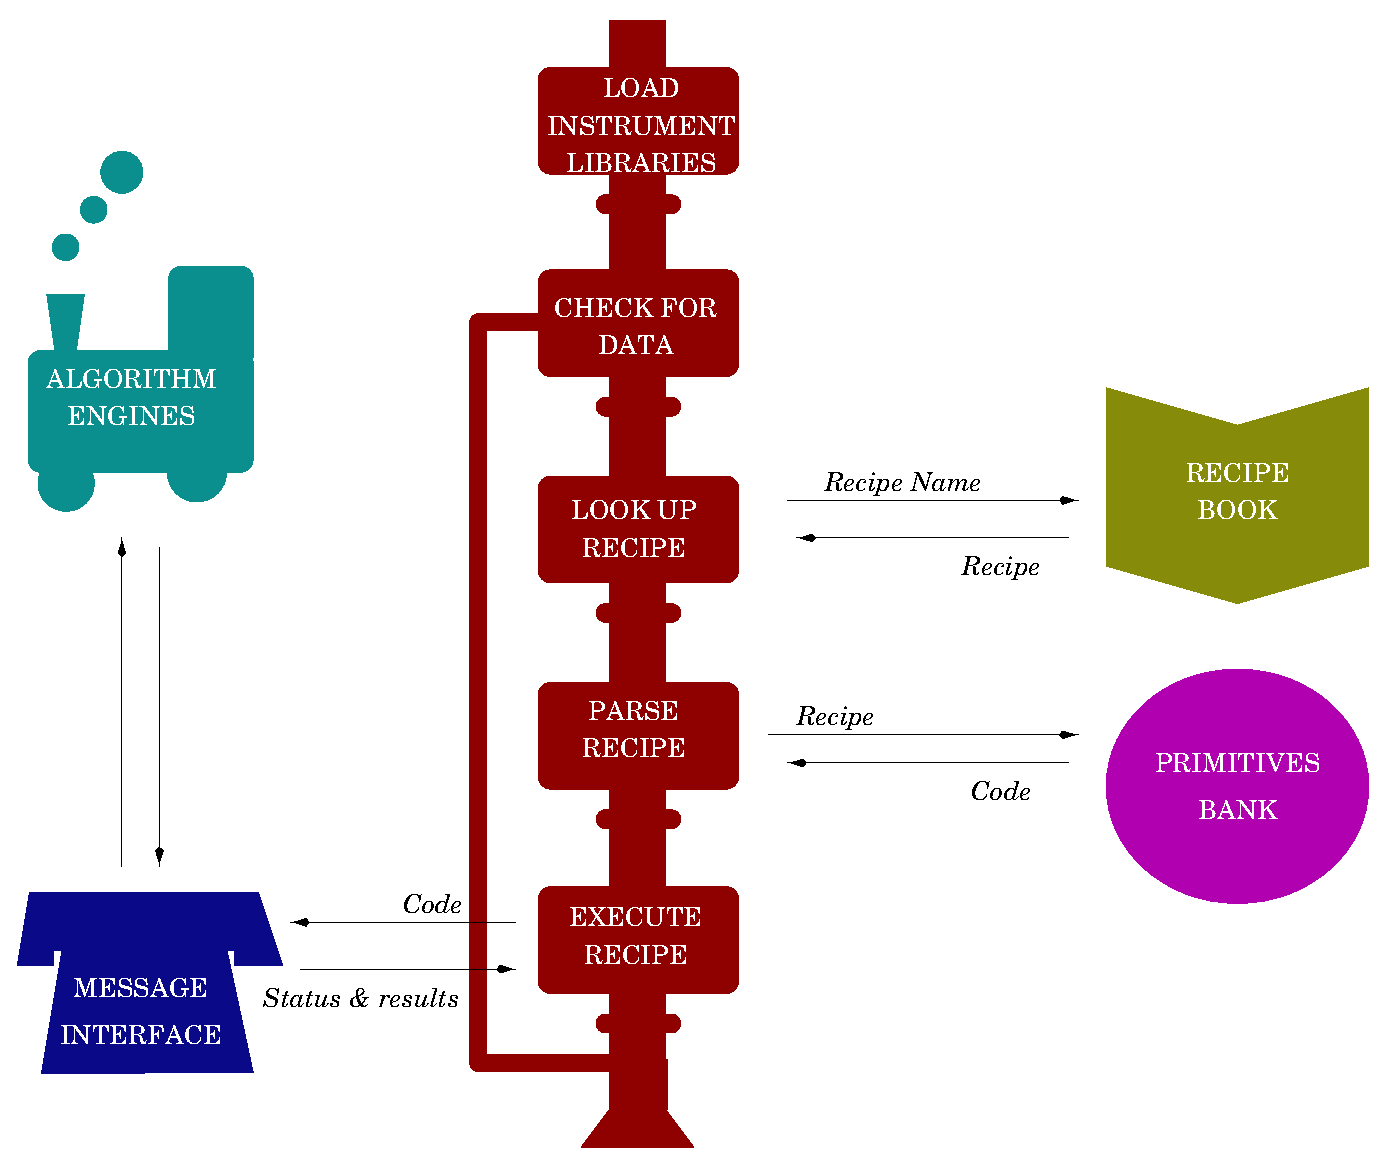
\includegraphics[width=\textwidth]{sun233_train}
\caption{Outline of the modularity of ORAC-DR}
\label{fig:train}
\end{figure}

This document provides information on writing recipes and for adding
support for new instruments to the pipeline.


\section{Recipes}

Recipes in \Oracdr\ consist of a series of data reduction steps
(primitives) containing instructions for the reduction of
data. In general, recipes are different for each instrument supported
and are keyed to the specific observing mode used to take the data.

An example recipe may look something like:

\begin{myquote}
\begin{verbatim}
=head1 NAME

RECIPE_NAME - Short description of what the recipe does

=head1 DESCRIPTION

Long description of what recipe does.

=head1 NOTES

Some notes associated with the recipe.

=head1 SEE ALSO

List of related recipes.

=head1 AUTHORS

List of authors

=cut

_INSTRUMENT_HELLO_
# A comment
_STEP_ONE_
_STEP_TWO_  ARG1=number ARG2=string
_STEP_THREE_
_TIDY_RECIPE_
\end{verbatim}
\end{myquote}

This recipe illustrates all the important features of a recipe:

\begin{itemize}
\item The recipe must contain documentation in the Perl POD syntax
(see e.g.\ the \textsc{perlpod} manpage). This documentation is used
by the \oracman\ command and for the automated documentation system.
At the very least, recipe documentation should include \textbf{NAME}
and \textbf{DESCRIPTION} fields. The \textbf{NAME} field should use
the standard Perl format of
\begin{myquote}
\begin{verbatim}
RECIPE_NAME - purpose
\end{verbatim}
\end{myquote}
so that the POD translators can correctly determine this information
when generating \LaTeX\ and HTML code.

\item To simplify the readability of recipes for non-programmers and
to separate the recipe language from the programming language
used to implement the primitives, \emph{no computer code should be visible
in the recipe}.\footnote{\Oracdr\ does not \emph{enforce} this rule
though and it is possible to include Perl constructs in private
recipes and for testing. It should not be done for production code.}

\item Recipes are in plain text, and are easily modified by both support
scientists and users with the aid of a text editor. This also means
that is should be easy to support a GUI based drag-and-drop-type
recipe builder at a future date.

\item For most instruments, it is required that a \textbf{HELLO}
primitive be included at the start of every recipe. This is used 
to guarantee that certain initialization steps are always
executed. See individual instrumentation documentation to see whether
a \textbf{HELLO} primitive is required.

\item The comment character is a \#. All text after a \# is ignored by 
the recipe parser.

\item Configuration options can be passed into primitives by the use
of a \texttt{KEYWORD=value} syntax. The recipe parser automatically
converts these values into arguments suitable for the primitives.


\item A \textbf{TIDY} primitive is required at the end of most
recipes. This can be used to remove intermediate files at the
end of a recipe and any other tidying operation It usually calls the
\primitive{\_DELETE\_TEMP\_FILES\_} primitive. It must make sure that
files required for subsequent group processing are not deleted.


\end{itemize}

Here is a more concrete example, the UFTI \texttt{QUADRANT\_JITTER} recipe
(without the pod sections and only minimal comments):

\begin{myquote}
\begin{verbatim}
# Initialisation
_IMAGING_HELLO_
_CREATE_WCS_
_QUADRANT_JITTER_HELLO_
_QUADRANT_JITTER_STEER_
# Calibration
_MASK_BAD_PIXELS_
_SUBTRACT_DARK_
_FLAT_FIELD_QUADRANT_JITTER_ MASK=1
# Mosaicking
_GENERATE_OFFSETS_QUADRANT_JITTER_ PERCENTILE=99 COMPLETE=0.4 MINPIX=12
_MAKE_MOSAIC_QUADRANT_OPTIMISED_ RESAMPLE=1 INT_METHOD=linint FILLBAD=1
# Cleanup
_QUADRANT_JITTER_TIDY_
\end{verbatim}
\end{myquote}


\subsection{Recipe Names}

The names of recipes should be descriptive. Short obtuse names are not
recommended since it should be obvious to the observer which recipe is
associated with which observing mode. In general, recipe names are
read from the file header, the location of which is specified by the
instrument specific classes in the \Oracdr. If required though, the
recipe can be specified on the command line although this can cause
problems if the user specifies the wrong observation numbers.

\subsection{Recipe locations}

\Oracdr\ searches in two locations for the recipe files. First, the directory
specified by the \texttt{ORAC\_\-RECIPE\_DIR} environment variable, if
defined, is searched. This allows users of the pipeline to modify a standard
recipe without editing the original. If the variable is not set or the recipe
can not be found, the default location of
\texttt{\$ORAC\_DIR/recipes/\$ORAC\_INSTRUMENT} is searched (although
\oracdr\ can sometimes be used to modify the value of
\texttt{ORAC\_INSTRUMENT} during initialization). The pipeline aborts if the
recipe cannot be located.



\section{Primitives}

\Oracdr\ primitives contain information for the manipulation of data in a
given state. They are written using object-oriented techniques,
manipulating objects associated with the individual data frames as
well as groups of observations. The steps that involve actual
processing of data (as opposed to housekeeping etc.\ tasks) are done via
a messaging request to an algorithm engine resident in memory.

Because primitives always manipulate objects associated with the
pipeline, they are order-ignorant, i.e.\ no assumptions are made about
the file number, file name, or filename convention. These behaviours
are all handled by instrument-specific classes, thus allowing the
possibility of changing these conventions for an instrument without
changing code and of re-use of primitives elsewhere in different
recipes for different instruments.

Additionally, it is possible for primitives to contain instructions to
include other primitives. An arbritrary limit of 10 levels is imposed
by the software to provide protection against recursion. This can
easily be extended if required but currently no recipes include
primitives at depths greater than 5.  The recipe parser recognises
primitive inclusion directives by matching the pattern \verb|^\s*_| in
non-pod sections, i.e.\ an underscore as the first blank character on a
line. The primitive directive should look exactly as it would if found
in a recipe, i.e.:
\begin{myquote}
\begin{verbatim}
 _SOME_PRIMITIVE_ ARG=arg  ARG2=$a  ARG3=$b
\end{verbatim}
\end{myquote}
and not
\begin{myquote}
\begin{verbatim}
 _SOME_PRIMITIVE_(ARG=arg, ARG2=$a, ARG3=$b);
\end{verbatim}
\end{myquote}
as would normally be expected for Perl. One difference from the recipe 
level\footnote{purely because the recipe level does not contain code} is that
Perl scalar variables can be used to pass values into the primitive
rather than having to hard-code a specific value. The current recipe
parser does not yet allow complex data structures (arrays, hashes,
objects, references) to be passed into primitives. This is because
of a desire to enforce simple interfaces to all primitives regardless
of location rather than an inability of the parser to be modified to
support it. If there is demand for it, this feature could easily be added.

The following variables are available to all primitives:

\begin{description}
\item[\$Frm] \mbox{} % $

  Object of class \texttt{ORAC::Frame} (or a subclass thereof). This
object contains information about the \emph{current} frame being
processed by the pipeline. Methods are provided for accessing the
current filename and the header information.

\item[\$Grp] \mbox{} % $

Object of class \texttt{ORAC::Group} (or a subclass thereof). This
object contains information about the \emph{current} group being
processed by the pipeline. In \Oracdr\ a group is thought of as an
array of frame objects. Methods are provided for accessing the current
filename and current group members. The current frame will be a member
of the current group. The usual behaviour is that the group object
will contain the frames processed so far that are part of the group,
in which case the last member of the group is the current frame.
Alternatively, it is possible for the group object to know about all
members of the group regardless of which have been processed already,
in which case the current frame may not necessarily be the last frame of
the group. The latter behaviour is controlled by the \texttt{-batch}
switch in \oracdr\ and can be used by primitive writers to delay group 
processing until the current frame is the last member of the group (a
group method is provided to determine this). This is only relevant for 
processing off-line but can significantly reduce run time of certain
recipes. Currently, SCUBA is the
only instrument that supports the batch option.

\item[\$Cal] \mbox{} %$

This provides access to the instrument's calibration system. This object
can return information such as the dark and flats to use for infrared
data or the current sky opacity for SCUBA. Extensive use is made of
index files and some primitives and recipes  must be responsible
for filing calibration data with this object so that later recipes
can access the correct information. The behaviour of this object is 
completely instrument specific, in general very few methods are
inherited by subclasses.

\item[\$Display] \mbox{} % $

An object of class \texttt{ORAC::Display}. Used by primitive writers
to send data display commands to the display subsystem. Note that
sending a display command does not necessarily result in anything
being displayed. The display system itself is not discussed in this document
[see the internals document].

\item[\%Mon] \mbox{}

A hash containing \texttt{ORAC::Msg} objects. These objects are used
to send messages to the algorithm engines. The hash keys will describe 
which algorithm engine is to be contacted. The instrument interface
should describe which tasks are available to programmers. Methods are
provided to send messages to algorithm engines (always waiting for the
reply before continuing) and for retrieving parameter values.

\item[\$ORAC\_PRIMITIVE] \mbox{} % $

This is the name of the current primitive. Usually used for debug
messages. Since this variable has a scope of the current primitive
only, if other primitives are included from within a primitive 
a new variable will be defined in the scope of the included
primitive. This will generate warnings if the \texttt{-w} switch
is turned on since the current variable will mask the variable defined
in the scope of the parent primitive (as desired).


\item[\%\_PRIMITIVE\_NAME\_] \mbox{}

Hash containing the arguments available to the current primitive. The
name of the hash is the same as the name of the primitive (i.e.\ the
hash is not named \texttt{\_PRIMITIVE\_NAME\_} explicitly).

\end{description}

All primitives (and in fact all of \Oracdr) are written with the 
\texttt{strict} pragma turned on (see \texttt{perldoc strict} for more 
information) primarily to force a declared scope for all variables.
All primitives are evaluated by the Perl interpreter as
\begin{myquote}
\begin{verbatim}
preamble added by the parser
{
  preamble added by the parser in limited scope
  _PRIMITIVE_
}
\end{verbatim}
\end{myquote}
such that each primitive is in a different block to all other
primitives\footnote{unless the primitive is nested inside another
primitive}. The only global variables used by primitives should be
those supplied by the pipeline, all other variables should be lexical
(i.e.\ using the Perl \texttt{my} declaration) and will therefore be
freed at the end of the primitive. Passing complex information between 
primitives must be achieved by other means and is discussed in
\S\ref{information_passing}. 

All recipes are evaluated in the \texttt{ORAC::Basic} namespace.
This fact should not be used by any primitives and it is not
guaranteed that this namespace will be used in future releases 
of \Oracdr. It can always be assumed that functions and methods from the
following modules will be visible to all primitives:

\begin{description}
\item[ORAC::Print] \mbox{}

Provides the \texttt{orac\_print}, \texttt{orac\_err} and
\texttt{orac\_warn} commands. These routines route messages to 
the correct output systems (an X-window, the screen, a log file etc)
specified by the user. The standard perl functions \texttt{print} and
\texttt{warn} should not be used for user messages except during
development since the user has no control of where to send them.

\item[ORAC::LogFile] \mbox{}

Used to write log files (see \S\ref{logfiles}).

\item[ORAC::Constants] \mbox{}

Provides access to the standard \Oracdr\ constants. The most important
are \texttt{ORAC\_\_OK} and \texttt{ORAC\_\_ERROR} (note that they 
are Perl constants, not variables).

\item[ORAC::TempFile] \mbox{}

Use to generate temporary files (see \S\ref{tempfiles}).

\item[ORAC::General] \mbox{}

Functions that are useful but are not necessarily a standard part of
Perl. Examples are \texttt{max()}, \texttt{min()} and \texttt{log10()}.

\end{description}


\section{Writing a Primitive}

In order to write a valid primitive certain steps must
be adhered to in order to ensure that subsequent primitives
have the correct information.

It assumes knowledge of the following Perl concepts:
using Perl objects, lexical variables, Perl data
structures. 

Here is an example primitive showing the basic principles:

\begin{myquote}
\begin{verbatim}
 1  =head1 NAME
 2
 3  _PRIMITIVE_NAME_ - short description
 4
 5  =head1 DESCRIPTION
 6 
 7  Long description
 8
 9  =head1 ARGUMENTS
10
11  =over 4
12
13  =item ARG1
14
15  Description of possible values of ARG1
16
17  etc...
18
19  =back
20
21  =head1 TASKS
22
23  List of external tasks required by the primitive
24
25  =head1 OUTPUT FILES
26
27  Output suffix for the display system.
28
29  etc, AUTHORS, COPYRIGHT.....
30
31  =cut
32
33  # Read arguments or use default values
34  my $arg1 = ( exists $_PRIMITIVE_NAME{ARG1} ? 
35               $_PRIMITIVE_NAME{ARG1} : 5);
36
37  # Loop over all sub frames
38  foreach my $i (1..$Frm->nfiles) {
39
40    # Get the input and output filename
41    my ($in, $out) = $Frm->inout('_sfx', $i);
42
43    # Read some value from the frame FITS header
44    my $value = $Frm->hdr('KEYWORD');
45
46    # Combine the in, out and value into options for the task
47    # DEPENDS ON ALGORITHM ENGINE
48    my $options = "IN=$in OUT=$out SWITCH=$value";
49
50    # Run the algorithm engine
51    $Mon{'task'}->obeyw('TASK',$options);
52
53    # Retrieve an answer from a parameter
54    ($ORAC_STATUS, $result) = $Mon{'task'}->get('TASK','PARAMETER');
55
56    # Print the result
57    orac_print "Result from primitive $ORAC_PRIMITIVE = $result\n";
58
59    # Update the frame object so that the next primitive
60    # gets the correct input file name
61    $Frm->file($i, $out);
62
63  }
64
65  # Ask the display system to display the frame
66  $Display->display_data($Frm) if defined $Display
67
\end{verbatim}
\end{myquote} %$
The following should be noted:
\begin{itemize}

\item Primitives are written in Perl and all variables are lexicals
(using \texttt{my}).

\item As for recipes, the first few lines (1--31) are the
documentation for the primitive in pod format. In addition to the
fields used for recipe headers, three new fields are required for
primitives, \textbf{ARGUMENTS} to describe the configuration options,
\textbf{TASKS} to list external dependencies and \textbf{OUTPUT FILES}
to list the suffix of any output data files (for use with the display
system) and any log files that may be written.

\item Supplied arguments can be read from the \_PRIMITIVE\_NAME\_
hash. Lines 33--35 check for the existence of the \texttt{ARG1}
key in the hash and read it if it exists else a default value is
copied in. Note the use of \texttt{exists} rather than
\texttt{defined} for checking hash contents. If \texttt{defined} is
used the key would automatically be created in the hash and set to a value of
\texttt{undef} whereas \texttt{exists} simply looks for the key in the 
hash without creating it. In general, this is the more correct
behaviour as it can distinguish between the key not being there at all 
(i.e.\ never set) and the key being set explicitly to
\texttt{undef}\footnote{Although it is not possible for a user to
specify a primitive argument value of \texttt{undef} this is still
good programming practice.}.

In some current primitives the following may
be found for reading arguments:
\begin{myquote}
\begin{verbatim}
my $arg1 = ( $_PRIMITIVE_NAME_{ARG1} || $default);
\end{verbatim}
\end{myquote} %$
This works in most normal cases but will fail if the value of the
argument is desired to be `0' since that evaluates to false and will
cause the default to be returned rather than a `0'. This construct
also causes the key to be created even if no argument was ever
supplied (known as \emph{auto-vivification}).

\item Line 38 starts a loop over all the sub-frames present in the
frame. The need for such a loop depends on the individual instrument.
UFTI, for example, only ever creates a single data frame per disk file
and so will not require the loop. SCUBA can take data for multiple
wavelengths, and MICHELLE can store multiple integrations per data
file, so this loop would ensure that each wavelength/integration is
processed in turn.

\item Line 41 retrieves the name of the current input file and
  supplies a valid output filename based on the supplied suffix,
  ``\texttt{\_sfx}''. Note that this command accepts a number as an
  optional argument. This can be used to connect the file name with
  the sub-frame (a Frame object can store multiple current filenames).

\item Line 44 simply retrieves a value from the header. The
\texttt{hdr()} method can also be used to set header values (but does
not change the header on disk).

\item Lines 46--51 send a message to an algorithm engine using a
messaging object stored in the \texttt{\%Mon} hash. The options
string depends on the task at the other end of the message bus and
will therefore need to be changed if the algorithm engine is changed.
An important point is that error checking code is automatically
inserted into the recipe when  \texttt{-$>$obeyw} is found in a line
that is not preceeded by an equals sign or a comment. This means that
line 51 is translated to:
\begin{myquote}
\begin{verbatim}
{
  my $OBEYW_STATUS = $Mon{'task'}->obeyw('TASK', $options);
  if ($OBEYW_STATUS != ORAC__OK) {
     < ERROR MESSAGE CONSTRUCTED AND PRINTED WITH orac_err>
     return $OBEYW_STATUS;
  }
}
\end{verbatim}
\end{myquote} %$
such that the recipe is aborted and an error message printed. Note
that this block runs in its own scope to prevent warnings from Perl
concerning the masking of previous \texttt{OBEYW\_STATUS} variables.

If automatic checking is not required, simply check the return
status. If the parser finds an equals sign before the \texttt{obeyw}
the line will not be re-written:

\begin{myquote}
\begin{verbatim}
my $status = $Mon{'kappa_mon'}->obeyw("stats","ndf=$in");
\end{verbatim}
\end{myquote} %$ 


\item Line 54 retrieves a parameter value from the external task.
This example also makes use of the automatic status checking within
\Oracdr. Whenever the parser sees the special \texttt{ORAC\_STATUS}
variable in a primitive, code is automatically added after this line to
check the value of \texttt{ORAC\_STATUS} and compare it with
\texttt{ORAC\_\_OK}. If the status is not good, the recipe aborts and an
error message is printed. This saves the primitive writer from having
to worry about status checking.

\item Line 57 makes use of the \texttt{orac\_print} command to send a
message to the user. The \texttt{orac\_print} command is written to
send the message to multiple output filehandles as defined by the user 
with the \texttt{-log} switch to \oracdr.

\item The final task in the loop (line 61) is to update the file name
  stored in the frame object. On exit from each primitive the frame
  and group objects must contain the filenames that should be used by
  subsequent primitives. This step is vital, and without it subsequent
  primitives will use the wrong input file names.

\item The final step is to display the reduced frames. The
\texttt{display\_data} method will ask for the current frame to be
displayed. Note that the display sub-system will \emph{only} display
the data frame if the user has requested this by configuring the
display system (using, for example, the \texttt{oracdisp} command)
accordingly. The check to make sure the display object is initialised
is required in case the user has turned off the display system.

\end{itemize}

\subsection{Log Files\label{logfiles}}

It is sometimes desirable to write results to log files as data
files are processed (for example, seeing statistics, pointing offsets
etc). Rather than force the primitive writer to check for the
existence of log files and decide whether or not to open or append to
log files, the \Oracdr\ system provides a simplified access to log
file creation via the \texttt{ORAC:LogFile} class.

All that is required to write an entry to a log file is for the
following methods to be invoked:
\begin{myquote}
\begin{verbatim}
my $log = new ORAC::LogFile('log.whatever');
$log->header(@header);
$log->addentry(@lines);
\end{verbatim}
\end{myquote} %$
The header will only be written to the log file if the log file
does not previously exist so it is safe to run this command in a
primitive without an explicit check. Both the \texttt{header()} and
\texttt{addentry()} methods accept arrays, and newline characters will
be appended to each item in the array when written to the log file.
The convention is that all log file names should start with `\texttt{log.}'.

\subsection{Temporary and intermediate files\label{tempfiles}}

In many cases, it is necessary to make use of temporary files
within a primitive, either for intermediate data steps that are not
relevant for the frame, or as text files input to external tasks. Since
these are not required once the primitive is finished a class is
provided for dealing with temporary files (\texttt{ORAC::TempFile}).

This class will choose a filename and, optionally, open the file ready 
for read-write access (when this facility is used it is guaranteed that the
file is unique and will not overwrite any existing file). The file,
and any files of the same name but with a \texttt{.sdf}
extension\footnote{the extension used for Starlink N-Dimensional data
format (NDF)}, are removed when the variable goes out of scope.

The only files that should remain when a primitive completes should be
those registered with the current frame or the current group. All
others should be temporary and should be tidied up on leaving the
primitive (which is automatic if \texttt{ORAC::TempFile} is
used)\footnote{This is not always a good idea when debugging. Future
  versions of the pipeline will disable the removal of temporary files 
  when the \texttt{-debug} flag is in use}.
This allows the final tidyup primitive to be responsible solely for
removing unwanted intermediate frames that were the product of
individual primitives (every time a the file name is updated in a
frame object the previous value is stored for possible later removal
by the tidy primitive). 

\subsection{Passing information between primitives\label{information_passing}}

Since each primitive is evaluated in its own scope, it is not possible 
(or even desirable) to pass simple variables between separate
primitives. Two means are provided for doing this:

\begin{itemize}
\item Using the \texttt{\%\_PRIMITIVE\_NAME\_} hash. The argument hash 
for each primitive is visible to all other primitives at the same
level.  This is because primitives are translated into:
\begin{myquote}
\begin{verbatim}
my %_PRIMITIVE_1_ = read_arguments( ... );
{
  _PRIMITIVE_1_
}
my %_PRIMITIVE_2_ = read_arguments( ... );
{
  _PRIMITIVE_2_
}
\end{verbatim}
\end{myquote}
This works but has a number of problems:
\begin{itemize}
\item The system breaks if the previous primitive is removed from the
recipe.\footnote{It will not simply return \texttt{undef}. The recipe
will fail to run since the hash would not have been declared previously.}
\item The system breaks if the primitive is renamed.
\item If the primitive from which data are required is in a different
scope from the current primitive this will not work.
\item It feels too much like a global variable\ldots
\end{itemize}

\item Store the information with the current frame or group object.
Both frame and group objects can use the \texttt{uhdr()} method to
store arbitrary data (including references) in a hash. This is the
recommended way of transferring data between primitives when the
information relates to the current frame or group. By convention, the
\texttt{hdr()} method should be used for storing FITS-like data.
Checks should be made for the existence of data in the hash before
using it.
\end{itemize}
The first method using the primitive hash only allows information to
be passed within the current recipe whereas the frame header allows
the information to be retained for subsequent frame processing.

\section{Calibration}

The calibration system is essentially based on the concept of index
files.  An index file is a data file containing information on all
calibration observation reduced by the pipeline. A separate index file
is created for each calibration sub-system (e.g.\ one for dark
observations, one for skydip observations etc) with the convention is
that each index file is stored in \texttt{ORAC\_DATA\_OUT} and
prefixed with the string \texttt{index} (e.g.\ \texttt{index.dark},
\texttt{index.skydip} etc.). It is the responsibility of a primitive
(usually a complete recipe is dedicated to the calibration
observation) to file a calibration to an index file. The index file
can be used simply to register a file name (e.g.\ the name of a dark file
or flatfield) or a calibration result (the current sky opacity or flux
conversion factor). Methods are provided in the \texttt{ORAC::Index}
class for retrieving this information from the index file\footnote{For
efficiency, the index file is kept in memory rather than read from
disk every time it is to be accessed. This means that \Oracdr\ is not
guaranteed to work if two processes are sharing a single ouput data
directory as this would cause problems with index file updates [they
are not locked].}

The index object is responsible for searching the relevant index
file and returning the most suitable calibration. This is achieved by
the use of external rules files (stored in \texttt{ORAC\_DATA\_CAL}
called \texttt{rules.CALIBRATION\_NAME}) which list which header
keywords are relevant and should be checked against the headers of the
current frame. This means that the calibration object itself does not
need to worry about searching the index file or reading the rules
files. 

An example rules file could look like:
\begin{myquote}
\begin{verbatim}
# Example rules file for SCUBA skydips
MODE eq 'SKYDIP'
FILTER eq $Hdr{FILTER}
WAVE == $Hdr{WAVE}
TAUZ
ORACTIME ; abs(ORACTIME - $Hdr{ORACTIME}) < 0.5
\end{verbatim}
\end{myquote} %$

The format is intended to be fairly simple as it should be possible
for a non-programmer to edit it. The main points are:

\begin{itemize}
\item \# is the comment character. Anything after a comment within a
  line is ignored.
\item Blank lines are ignored.
\item Each line in the rules file is translated to the Perl code and
evaluated. If it returns `true' the value in the index file (keyed by
the first word in the rules file) matches the coresponding values in
the header of the current frame. For example, the second rule
is translated into the following code (assuming the current index
entry contains the filter name of "850W").

\begin{myquote}
\begin{verbatim}
if ( '850W' eq $Hdr{FILTER} ) {
   # Rules passes
}
\end{verbatim}
\end{myquote}
and the last line in the above rules file could be translated to the
following \texttt{if} statement (using ORACTIME of 19990827.55 for the
index entry):
\begin{myquote}
\begin{verbatim}
'19990827.55'; abs(19990827.55 - $Hdr{ORACTIME}) < 0.5 
\end{verbatim}
\end{myquote} %$
which returns true if the \texttt{ORACTIME} stored in the index is
within half a day of the value stored in the current frame object
(\%Hdr is a hash read from the current frame header).
The semi-colon is used to separate the Perl code into two statements.
The return value of the \texttt{eval} is that of the second statement. This is
required for cases that are not simply `\texttt{A == B}' format.
\item When using complex rules the substituted index value (ORACTIME
  in the above example) is only quoted when
placed as the first statement. When in the body of the rule it must be 
quoted if the value is not a number. This is because the value itself
is placed into the rule rather than a variable containing the value.
\item Lines which only contain a keyword, are place holders indicating
that the information should be present in the index file but not used.
Care must be taken that the value of the corresponding keyword can never
be zero since that would return false to the rules system. If this is the 
case a rule of
\begin{myquote}
\begin{verbatim}
KEYWORD ; 1
\end{verbatim}
\end{myquote}
can be used instead since in this case the test will always return true.
\end{itemize}

\subsection{Calibration overrides}

\ORACDR\ gives the user the ability to override the default calibration
information as returned by the pipeline through use of the \texttt{-calib}
commandline option. By adding methods in \texttt{ORAC::Calib} or in
instrument-specific subclasses, it is possible to add various override
methods. As an example of this, see the \texttt{profile}, \texttt{profilename},
\texttt{profileindex}, and \texttt{profilenoupdate} methods in
\texttt{ORAC::Calib::CGS4}. For further information on adding override
methods see \S\ref{calibration_add}, and for information on using
override methods when reducing data with \Oracdr\ see SUN/230.

A number of general overrides are available. 

\begin{itemize}

\item baseshift - Use the given comma separated doublet (i.e. ``0,0'') as the
frame's base position.

\item bias - Use the given bias frame.

\item dark - Use the given dark frame.

\item flat - Use the given flat frame.

\item mask - Use the given mask. Usually used for bad pixel masks.

\item readnoise - Use the given value for the detector readnoise.

\item rotation - Use the given frame as a rotation matrix.

\item sky - Use the given sky frame.

\item standard - Use the given standard star frame.

\end{itemize}

\section{Message output}

The \oracdr\ infrastructure provides commands for primitive writers
to print informational messages, warnings and error messages to the
user. These commands are \texttt{orac\_print}, \texttt{orac\_warn},
and \texttt{orac\_err}. In principal these commands can send
information to different locations and this location is under the control of
the person running the pipeline rather than primitive writer (using
the \texttt{-log} option). The Perl \texttt{print} and \texttt{warn}
commands should not be used since they always write output to standard 
output and standard error whereas the ORAC print commands can send to
multiple filehandles.

\section{Recipe Debugging}

Some facilities are provided to ease the debugging of recipes and
primitives. These are as follows.

\begin{itemize}

\item When a recipe will not compile (due to syntax errors, for
example) the pipeline aborts and the error message and a listing of
relevant recipe lines (the version of the recipe executed internally
with all the extra code inserted) is printed to the screen.

\item The \texttt{-w} switch should be used during development 
in order to trap and fix any warnings detected by the Perl interpreter
at runtime. In many cases, these warnings are indicative of code that
makes assumptions about state (warnings on use of \texttt{undef}) or
scope (\texttt{my} declarations masking variables defined in a higher
scope). 

If warnings are raised from the \Oracdr\ core please contact the
authors and they will be fixed.\footnote{currently the one known issue 
is multiple declarations of the \texttt{ORAC\_PRIMITIVE} variable.}

\item The \texttt{-verbose} switch can be used to turn on messages from 
the algorithm engines. This is sometimes useful to make sure that the
external task is doing the expected operation.

\item The \texttt{oracdr\_parse\_recipe} command is provided to translate
a recipe into Perl code. It takes a recipe name as argument and sends the
translated recipe to standard output. This command can be used to check the
syntax of the recipe (by compiling the perl code and exiting immediately)
by using the \texttt{--syntax} option.

\item The final option is to turn on full debugging with the
\texttt{-debug} switch. This creates a file in
\texttt{ORAC\_DATA\_OUT} called \texttt{ORACDR.DEBUG} containing the
contents of each message sent to external tasks with an
\texttt{obeyw}. This can be used to find out what the final message
sent to a task was before the recipe crashed. If a
recipe crashes when the debugging is turned on the full contents of
the recipe buffer (i.e.\ the fully parsed recipe) will also be written 
to a file in \texttt{ORAC\_DATA\_OUT} called
\texttt{ORACDR\_RECIPE.dump}. This would be identical to running the
\texttt{oracdr\_parse\_recipe} command.

\end{itemize}

The Perl debugger should be used with care since it is possible to
hang the message bus if the program is frozen during a message
transaction and the debugger is not optimized for use with the use of nested
\texttt{eval} common in the pipeline internals.

\section{Adding new instruments}

Adding a new instrument to \Oracdr\ requires a number of steps, the
complexity of which will depend on how close the instrument is to an
instrument that is already supported by the pipeline.

This section describes the areas that must be modified to support a
new instrument. It assumes knowledge of the following Perl concepts:
writing object-oriented modules, lexical variables, Perl data
structures and \texttt{eval}. Message system interfaces will also
require a knowledge of Perl XS.


\subsection{Frames}

An \texttt{ORAC::Frame} class is responsible for filename conventions
and handling of sub-frames. The most common methods that need to be
sub-classed are:

\begin{description}
\item[new()] \mbox{}

The object constructor should be modified to set the default behaviour
for \texttt{rawfixedpart()}, (the part of the filename that does not
change with UT date of observation number), \texttt{rawsuffix()},
(the file suffix of the raw data file),
\texttt{rawformat()} (the input format of the data: FITS, NDF etc.)
and \texttt{format()} (the data format required by the algorithm
engines).

The base constructor (\texttt{SUPER::new()}) should be invoked to
instantiate the object.

\item[calc\_orac\_headers()] \mbox{}

This method is used to translate instrument specific headers to those
required by the pipeline. Currently this method must insert the
following  keywords into the frame header.

\begin{description}
\item[ORACUT] \mbox{}

This should be the UT date of the observation in YYYYMMDD format.

\item[ORACTIME] \mbox{}

This should be the UT date and time of the observation in
YYYYMMDD.frac format (i.e.\ UT date plus fraction of day). This is
used by the calibration system to ensure that a guaranteed time stamp
can be used for comparison in index files.

\end{description}

\item[file\_from\_bits()] \mbox{}

Given a UT date  and an observation number, return the name of the 
raw data file. This is used by the pipeline to look for the file on disk.

\item[flag\_from\_bits()] \mbox{}

Given a UT date and an observation number, return the name of the flag 
file. This is used by the pipeline to search for a completion flag on
disk associated with the current observation file. Only required if 
it is intended for the pipeline to be used in conjunction with the 
\texttt{-loop flag} option.

\item[findgroup()] \mbox{}

Translates the header values into a group name and updates the frame.

\item[findrecipe()] \mbox{}

Translates the header values into a recipe name and updates the frame.

\item[template()] \mbox{}

Modifies the current filename so that it matches the filename that you 
would have had at an earlier point in the reduction when the
supplied template was valid. This is used for jumping to earlier steps
in the reduction when performing group operations.
Currently this method is generally
implemented by replacing the suffix with the supplied value. It could
also be implemented by accessing the list of prior file names with the
\texttt{intermediates()} method.

\item[inout()] \mbox{}

Given a suffix and sub-frame number provide a recommended name for the 
output file. Does not update the frame object. In general, this can
either simply append the suffix or replace the last suffix. The latter 
is normal practice.

\end{description}

In addition to those listed above, some methods need to know something
about the file format and should be modified (most UKIRT and JCMT
instruments inherit from the \texttt{ORAC::Frame::NDF} class rather
than \texttt{ORAC::Frame} since that class knows how to read from NDF
files). The automatic format conversion will have occurred before
these methods need to be run (for example if the input format is FITS
but the processing format is NDF, then the methods should be written
assuming NDF files). These methods are as follows.

\begin{description}

\item[readhdr()] \mbox{}

Reads the file header and stores the resulting hash reference in the
object. Also forces the ORAC headers to be calculated.

\item[erase()] \mbox{}

A method to delete the file currently associated with the frame. This
is effectively and \texttt{unlink()} but for NDF files the
\texttt{.sdf} is appended. The base class implementation can be used
in most cases.

\item[file\_exists()] \mbox{}

Checks to see if the data file exists. There is a special case for NDF format
since the \texttt{.sdf} extension is not present in the file name.

\item[stripfname()] \mbox{}

Strips the extension from the filename. The base class does nothing to 
the filename.

\end{description}

Finally, any extra methods not present in the base class but required
by an instrument should also be added. These can cover translation of
wavelengths to sub-frame filename, for example (used by the SCUBA class).

\subsubsection{Frame headers}

There are a number of internal headers that ORAC primitives rely on
to correctly reduce data. These headers are retrieved from the files
and translated to be used by oracdr. These headers can be used in 
recipes through the \texttt{ORAC::Frame::uhdr()} method and prepending 
ORAC\_ to each header. For example, to refer to the \texttt{INSTRUMENT}
header in a primitive, you would use

\begin{verbatim}

my $Frm = new ORAC::Frame('filename.sdf');
my $instrument = $Frm->uhdr('ORAC_INSTRUMENT');

\end{verbatim}

New internal headers can always be created, if necessary, to define
some ancillary data needed by a recipe, in an instrument-independent
fashion.

The following headers currently exist.  Note that not all headers are
defined for each instrument or recipe.

\begin{description}

\item[AIRMASS\_START] \mbox{}

Airmass at start of the observation (for a mosaic) or integration (for
a raw frame).

\item[AIRMASS\_END] \mbox{}

Airmass at end of the observation (for a mosaic) or integration (for
a raw frame).

\item[CHOP\_ANGLE] \mbox{}

Position angle of the chop (in degrees).

\item[CHOP\_THROW] \mbox{}

Throw of the chop with respect to the middle position (in arcseconds).

\item[CONFIGURATION\_INDEX] \mbox{}

Configuration index.  Increments when an instrument's hardware
configuration changes.

\item[DEC\_BASE] \mbox{}

Declination (ORAC\_EQUINOX equinox) at the reference position at zero
offset (in degrees).  The reference position is normally at the array
centre, but may be displaced, for example, to avoid the intersections
of abutted detector sub-arrays.

\item[DEC\_SCALE] \mbox{}

Pixel increment along declination axis (in arcsec).

\item[DEC\_TELESCOPE\_OFFSET] \mbox{}

Telescope declination offset with respect to the base position
given by DEC\_BASE (in arcseconds).

\item[DETECTOR\_BIAS] \mbox{}

Detector bias voltage (in volts)

\item[DETECTOR\_INDEX] \mbox{}

Position number in detector scan.

\item[DETECTOR\_READ\_TYPE] \mbox{}

Observing mode, such as \texttt{STARE}, \texttt{NDSTARE}, \texttt{CHOP}.

\item[EQUINOX] \mbox{}

Equinox of object position (in years).  It should be \texttt{2000}.

\item[EXPOSURE\_TIME] \mbox{}

Integration time per exposure (in seconds).

\item[FILTER] \mbox{}

Combined filter name.

\item[GAIN] \mbox{}

Detector gain (in electrons/ADU).

\item[GRATING\_DISPERSION] \mbox{}

Grating dispersion (in microns/pixel).

\item[GRATING\_NAME] \mbox{}

Grating name.

\item[GRATING\_ORDER] \mbox{}

Grating order.

\item[GRATING\_WAVELENGTH] \mbox{}

Grating wavelength (in microns).

\item[INSTRUMENT] \mbox{}

Instrument name.

\item[NSCAN\_POSITIONS] \mbox{}

Number of scan positions in scan.

\item[NUMBER\_OF\_EXPOSURES] \mbox{}

Number of exposures in integration.

\item[NUMBER\_OF\_OFFSETS] \mbox{}

Number of jitter offset positions in an observation.

\item[NUMBER\_OF\_READS] \mbox{}

Number of reads per exposure.

\item[OBJECT] \mbox{}

Object name from telescope.

\item[OBSERVATION\_MODE] \mbox{}

Camera mode, such as \texttt{imaging} or \texttt{spectroscopy}. 
Used for multi-mode instruments like Michelle.

\item[OBSERVATION\_NUMBER] \mbox{}

Observation number.  Observation numbers normally commence at \texttt{1}
for each night.

\item[OBSERVATION\_TYPE] \mbox{}

Observation type.  Used to determine whether observation is of the
\texttt{OBJECT}, \texttt{DARK}, or ARC, for example.

\item[RA\_BASE] \mbox{}

Right Ascension (ORAC\_EQUINOX equinox) at the reference position at
zero offset (in degrees).  See DEC\_SCALE.

\item[RA\_SCALE] \mbox{}

Pixel increment along right-ascension axis (in arcsec).

\item[RA\_TELESCOPE\_OFFSET] \mbox{}

Telescope right-ascension offset with respect to the base position
given by RA\_BASE (in arcseconds).

\item[ROTATION] \mbox{}

Angle of declination axis with respect to the second ($y$) axis, measured
counterclockwise (in degrees).

\item[SCAN\_INCREMENT] \mbox{}

Increment between scan positions (in pixels).

\item[SLIT\_ANGLE] \mbox{}

Position angle of slit (in degrees)

\item[SLIT\_NAME] \mbox{}

Name of slit.

\item[SPEED\_GAIN] \mbox{}

Readout speed.  The default is \texttt{Normal}.

\item[STANDARD] \mbox{}

Is the target a standard-star observation?

\item[UTDATE] \mbox{}

UTC date when the observation was made.

\item[UTEND] \mbox{}

End time of integration (for raw data) or the observation (for a
mosaic).

\item[UTSTART] \mbox{}

Start time of integration (for raw data) or the observation (for a
mosaic).

\item[WAVEPLATE\_ANGLE] \mbox{}

Polarimeter waveplate position angle (in degrees).

\item[X\_DIM] \mbox{}

Number of detectors in a readout column (in pixels).

\item[Y\_DIM] \mbox{}

Number of detectors in a readout row (in pixels).

\item[X\_LOWER\_BOUND] \mbox{}

Start column of array readout.

\item[X\_UPPER\_BOUND] \mbox{}

End column of array readout.

\item[Y\_LOWER\_BOUND] \mbox{}

Start row of array readout.

\item[Y\_UPPER\_BOUND] \mbox{}

End row of array readout.

\end{description}

\subsection{Groups}

An \texttt{ORAC::Group} class is responsible for dealing with groups
of frame objects and with an output group data file.
The most common methods that need to be sub-classed are given below.

\begin{description}

\item[new()] \mbox{}

The constructor must be overridden to specify the type fixed part and
file suffix of the output group file. The base constructor should be
used from the subclass to instantiate the object.

\item[readhdr()/erase()/file\_exists()/file\_from\_bits()] \mbox{}

Similar to the frame implementations.


\end{description}

For specialized applications it may also be necessary to implement 
the \texttt{coaddswrite()}/\texttt{coaddsread()} methods. These will
be used by the CGS4/MICHELLE instrument classes to allow coadds to be 
combined part way through a group without having to re-reduce earlier
observations. Not all instruments require support for this.

\subsection{Calibration}\label{calibration_add}

For a new instrument all that is required is to specify a new
set of rules and work out what to do with the `best' calibration that
is returned. For UFTI this simply means that the name is returned to
the primitive for use. For SCUBA more complex routines are required
for sky opacity calibration since the number returned by the index
file is sometimes modified for different filters before being returned 
to the user (the SCUBA calibration system never returns a file name).

For every type of calibration, the calibration object
(\texttt{ORAC::Calib} and sub-classes) must provide the following methods:
\begin{enumerate}
\item A method for returning the current calibration observation that
matches the criteria. This method should be an obvious name related
directly to the calibration (e.g.\ `dark', `skydip').
\item A method for retrieving the \texttt{ORAC::Index} object
associated with the relevant index file. The name of this method
should be related to the name of the index file (e.g.\
\texttt{skydipindex} will access the file \texttt{index.skydip}).
\item A method to prevent the pipeline from overwriting the current
calibration (used when the user is overriding a certain calibration
from the command line). This will be called, for example,
\texttt{darknoupdate()}. \oracdr\ assumes that the method
is of this form since this method will be called whenever a user
makes use of the \texttt{-calib} switch,

\end{enumerate}



\subsection{Algorithm Engines}

Each instrument requires its own implementation of an
\texttt{ORAC::Inst} module. This module is responsible for
implementing the commands for starting the messaging layer (if
required) and launching external tasks ready for use by the
pipeline. It may be possible for future releases to launch
external tasks on demand the first time an \texttt{obeyw} is
issued but this depends on the implementation of the messaging class and 
still requires that an object for each class is instantiated in the
\texttt{ORAC::Inst} module at startup.

Currently, this module is not object-oriented. This may change in the
future.

Another factor related to the algorithm engines is the implementation
of the messaging interface. The current interface is to the 
ADAM messaging system used by Starlink. An additional interface is
provided to run ADAM tasks via the Unix shell as a proof of concept.
Interfaces to Glish and IRAF will be needed to talk to \textsc{aips++}
and \textsc{Iraf} tasks. A Perl-to-DRAMA interface exists and it
should be fairly simple to write an \Oracdr\ interface for
DRAMA tasks. A shell interface should be used as a last
resort and only if valid exit status can be returned to the pipeline.



\subsection{\oracdr}

Once the instrument classes have been written, \oracdr\ needs to be
modified so that it can interpret a new value for
\texttt{ORAC\_INSTRUMENT} and configure the frame, group and
calibration objects correctly.

In the future this configuration may be moved into an external data
file so that the core \oracdr\ routine need not be modified by people
porting the system to a new instrument.

\subsection{Recipes}

Once \Oracdr\ has been configured to recognise the new instrument, the 
final step is to write the recipes and associated primitives to deal
with the new data and possibly new algorithm engines. At its simplest, 
for example for an infrared image, this may simply require copying
pre-written primitives from an existing instrument\footnote{Plans are
ongoing to allow multiple search paths for recipes and primitives so
that single copies can be used by multiple instruments without having
to copy the files to separate locations}.
At its most complex, completely new primitives will have to be written.

\appendix

\section{Directory Layout}

\Oracdr\ is designed to include all its directories in a single
location and not to care where that location is. All \Oracdr\ software
is located relative to the directory described by  the \texttt{ORAC\_DIR}
environment variable.

The standard layout is as follows.

\begin{description}
\item[bin] \mbox{}

Executable programs. This includes \oracdr, \oracman\ and others. Note
that none of the programs that form part of \Oracdr\ are binary. 
The core \Oracdr\ system will run anywhere the necessary Perl modules
are available.

\item[recipes] \mbox{}

All the recipe files. Contains a directory for each instrument (using
upper case) usually matching the value of the
\texttt{ORAC\_INSTRUMENT} environment variable.

\item[primitives] \mbox{}

All the primitive files. Contains a directory for each instrument
(using upper case) usually matching the value of the
\texttt{ORAC\_INSTRUMENT} environment variable.

\item[howto] \mbox{}

Basic introductory documentation for \Oracdr.

\item[lib] \mbox{}

Library files required by \Oracdr. Contains a \texttt{perl5} directory
with all the Perl modules used by the system. The \texttt{perl5}
directory is the usual value for the \texttt{ORAC\_PERL5LIB}
environment variable.

\item[images] \mbox{}

Image files used by the system. Contains the start up images for the
display tools (in NDF format).

\item[docs] \mbox{}

Main documentation. Contains a directory per document. Currently
contains all the Starlink User Notes.

\item[gui] \mbox{}

Graphical user interface definitions. Only used by \oracdisp.

\end{description}

\section{Perl Bibliography}

The following Perl books are recommended for more information on the
Perl features described in this document:

\begin{description}

\item[Programming Perl] 3rd edition, Wall, Christiansen and Orwant,
  2000, O'Reilly and Associates.

\item[Advanced Perl Programming] Srinivasan, 1997, O'Reilly and Associates.

\item[Object-Oriented Programming in Perl] Conway, 1999, Manning

\end{description}


%%%%%%%%%


%%%% INSERT ShellVariables pod here

%%%%%%%%

\section{Class libraries}

This section describes the class libraries that are relevant for
a recipe writer.

\subsection{ORAC::Calib\label{ORAC::Calib}\index{ORAC::Calib}}


Base class for selecting calibration frames in ORAC-DR

\subsubsection*{SYNOPSIS\label{ORAC::Calib_SYNOPSIS}\index{ORAC::Calib!SYNOPSIS}}
\begin{verbatim}
  use ORAC::Calib;
\end{verbatim}
\begin{verbatim}
  $Cal = new ORAC::Calib;
\end{verbatim}
\begin{verbatim}
  $dark = $Cal->dark;
  $Cal->dark("darkname");
\end{verbatim}
\begin{verbatim}
  $Cal->standard(undef);
  $standard = $Cal->standard;
  $bias = $Cal->bias;
\end{verbatim}
\subsubsection*{DESCRIPTION\label{ORAC::Calib_DESCRIPTION}\index{ORAC::Calib!DESCRIPTION}}


This module provides the basic methods available to all ORAC::Calib
objects.  This class should be used for selecting calibration frames.



Unless specified otherwise, a calibration frame is selected by first,
the nearest reduced frame; second, explicit specification via the
-calib command line option (handled by the pipeline); third, by search
of the appropriate index file.



Note this version: Index files not implemented.

\subsubsection*{PUBLIC METHODS\label{ORAC::Calib_PUBLIC_METHODS}\index{ORAC::Calib!PUBLIC METHODS}}


The following methods are available in this class.

\paragraph*{Constructors\label{ORAC::Calib_Constructors}\index{ORAC::Calib!Constructors}}
\begin{description}

\item[{\textbf{new}}] \mbox{}

Create a new instance of a ORAC::Calib object.
The object identifier is returned.

\begin{verbatim}
  $Cal = new ORAC::Calib;
\end{verbatim}
\end{description}
\paragraph*{Accessor Methods\label{ORAC::Calib_Accessor_Methods}\index{ORAC::Calib!Accessor Methods}}
\begin{description}

\item[{\textbf{thing}}] \mbox{}

Returns the hash that can be used for checking the validity of
calibration frames. This is a combination of the two hashes
stored in \texttt{thingone} and \texttt{thingtwo}. The hash returned
by this method is readonly.

\begin{verbatim}
  $hdr = $Cal->thing;
\end{verbatim}

\item[{\textbf{thingone}}] \mbox{}

Returns or sets the hash associated with the header of the object
(frame or group or whatever) needed to match calibration criteria
against.



Ending sentences with a preposition is a bug.


\item[{\textbf{thingtwo}}] \mbox{}

Returns or sets the hash associated with the user defined header of
the object (frame or group or whatever) against which calibration
criteria are applied.

\end{description}
\paragraph*{General Methods\label{ORAC::Calib_General_Methods}\index{ORAC::Calib!General Methods}}
\begin{description}

\item[{\textbf{find\_file}}] \mbox{}

Returns the full path and filename of the requested file (the first
file found in the search path).

\begin{verbatim}
  $filename = $Cal->find_file("fs_izjhklm.dat");
\end{verbatim}


croaks if the file can not be found. It's likely that this is a bit
drastic but it will indicate something bad is going on before some
other unexpected behaviour occurs.  See
\textbf{ORAC::Inst::Defn::orac\_determine\_calibration\_search\_path} for
information on setting up calibration directories.


\item[{\textbf{retrieve\_by\_column}}] \mbox{}

Returns the value for the specified column in the specified index.

\begin{verbatim}
  $value = $Cal->retrieve_by_column( "readnoise", "ORACTIME" );
\end{verbatim}


The first argument is a queryable

\end{description}
\subsubsection*{DYNAMIC METHODS\label{ORAC::Calib_DYNAMIC_METHODS}\index{ORAC::Calib!DYNAMIC METHODS}}


These methods create methods for the standard calibration schemes for subclasses.
By default calibration "xxx" needs to create standard accessors for "xxxnoupdate",
"xxxname" and "xxxindex".

\begin{description}

\item[{\textbf{GenericIndex}}] \mbox{}

Helper routine that creates an index object and returns it. Updates the
object based on the root name.

\begin{verbatim}
 $index = $Cal->CreateIndex( "flat", "dynamic" );
\end{verbatim}


Where the first argument should match the root name of the index and rules
file. The second argument can have three modes:

\begin{verbatim}
  dynamic - index file is assumed to be in ORAC_DATA_OUT
  static  - index file is assumed to be in the calibration tree
  copy    - index file will be copied to ORAC_DATA_OUT from
            ORAC_DATA_CAL if not present in ORAC_DATA_OUT
\end{verbatim}


If a third argument is supplied it is assumed to be an ORAC::Index
object to be stored in the calibration object.


\item[{\textbf{GenericIndexAccessor}}] \mbox{}

Generic method for retrieving or setting the current value based on index
and verification. Uses ORACTIME to verify.

\begin{verbatim}
  $val = $Cal->GenericIndexAccessor( "sky", 0, 1, 0, 1, @_ );
\end{verbatim}


First argument indicates the root name for methods to be called. ie "sky" would
call "skyname", "skynoupdate", and "skyindex".



Second argument controls whether the time comparison should be
nearest in time (0), or earlier in time (-1).



Third argument controls croaking behaviour. False indicates that the method
should croak if a suitable calibration can not be found. True indicates
that it should return undef. If a code ref is provided, it will be executed
if no suitable calibration is found. If it returns a defined value it
will be assumed to be a valid match, and if it returns undef the method
will croak as no suitable calibration will be available. This allows defaults
to be inserted.



Fourth argument controls whether calibration object verification is
not done.



Fifth argument controls whether warnings are displayed when searching
through the index file for a suitable calibration. Default is to warn.

\begin{verbatim}
  $val = $Cal->GenericIndexAccessor( "mask", 0, sub { return "bpm.sdf" }, @_ );
\end{verbatim}

\item[{\textbf{GenericIndexEntryAccessor}}] \mbox{}

Like \texttt{GenericIndexAccessor} except that a particular value from the index
is retrieved rather than a indexing key (filename).



No verification is performed.

\begin{verbatim}
  $val = $Cal->GenericIndexAccessor( "sky", "INDEX_COLUMN", @_ );
\end{verbatim}


First argument indicates the root name for methods to be called. ie "sky" would
call "skycache", "skynoupdate", and "skyindex".



If a reference to an array or columns is given in argument 2, all values
are checked and the row reference is returned instead of a single value.

\begin{verbatim}
  $entryref = $Cal->GenericIndexAccessor( "sky", [qw/ col1 col2 /], @_ );
\end{verbatim}

\item[{\textbf{CreateBasicAccessors}}] \mbox{}

Dynamically create default accessors for "xxxnoupdate", "xxxname" and "xxxindex" methods.

\begin{verbatim}
 __PACKAGE__->CreateAccessors( "xxx", "yyy", "zzz" );
\end{verbatim}
\end{description}
\subsubsection*{SEE ALSO\label{ORAC::Calib_SEE_ALSO}\index{ORAC::Calib!SEE ALSO}}


\emph{ORAC::Group} and
\emph{ORAC::Frame}

\subsubsection*{REVISION\label{ORAC::Calib_REVISION}\index{ORAC::Calib!REVISION}}


\$Id\$

\subsubsection*{COPYRIGHT\label{ORAC::Calib_COPYRIGHT}\index{ORAC::Calib!COPYRIGHT}}


Copyright (C) 1998-2004 Particle Physics and Astronomy Research
Council. All Rights Reserved.

\subsection{ORAC::Calib::SCUBA\label{ORAC::Calib::SCUBA}\index{ORAC::Calib::SCUBA}}


SCUBA calibration object

\subsubsection*{SYNOPSIS\label{ORAC::Calib::SCUBA_SYNOPSIS}\index{ORAC::Calib::SCUBA!SYNOPSIS}}
\begin{verbatim}
  use ORAC::Calib::SCUBA;
\end{verbatim}
\begin{verbatim}
  $Cal = new ORAC::Calib::SCUBA;
\end{verbatim}
\begin{verbatim}
  $gain = $Cal->gain($filter);
  $tau  = $Cal->tau($filter);
  @badbols = $Cal->badbols;
\end{verbatim}
\subsubsection*{DESCRIPTION\label{ORAC::Calib::SCUBA_DESCRIPTION}\index{ORAC::Calib::SCUBA!DESCRIPTION}}


This module returns (and can be used to set) calibration information
for SCUBA. SCUBA calibrations are used for extinction correction
(the sky opacity) and conversion of volts to Janskys.



It can also be used to set and retrieve lists of bad bolometers generated
by noise observations.



This class does inherit from \textbf{ORAC::Calib} although nearly all the
methods in the base class are irrelevant to SCUBA (this class only
uses the thing() method).

\subsubsection*{PUBLIC METHODS\label{ORAC::Calib::SCUBA_PUBLIC_METHODS}\index{ORAC::Calib::SCUBA!PUBLIC METHODS}}


The following methods are available in this class.
These are in addition to the methods inherited from \textbf{ORAC::Calib}.

\paragraph*{Constructor\label{ORAC::Calib::SCUBA_Constructor}\index{ORAC::Calib::SCUBA!Constructor}}
\begin{description}

\item[{\textbf{new}}] \mbox{}

Create a new instance of a ORAC::Calib::SCUBA object.
The object identifier is returned.

\begin{verbatim}
  $Cal = new ORAC::Calib::SCUBA;
\end{verbatim}
\end{description}
\paragraph*{Accessor Methods\label{ORAC::Calib::SCUBA_Accessor_Methods}\index{ORAC::Calib::SCUBA!Accessor Methods}}
\begin{description}

\item[{\textbf{default\_fcfs}}] \mbox{}

Return the default FCF lookup table indexed by filte.

\begin{verbatim}
 %FCFS = $cal->default_fcfs();
\end{verbatim}

\item[{\textbf{secondary\_calibrator\_fluxes}}] \mbox{}

Return the lookup table of fluxes for secondary calibrators.

\begin{verbatim}
 %photfluxes = $cal->secondary_calibrator_fluxes();
\end{verbatim}

\item[{\textbf{badbols}}] \mbox{}

Set or retrieve the name of the system to be used for bad bolometer
determination. Allowed values are:

\begin{itemize}

\item index

Use an index file generated by noise observations
using the reflector blade. The bolometers stored in this
file are those that were above the noise threshold in 
the \_REDUCE\_NOISE\_ primitive. The index file is generated
by the \_REDUCE\_NOISE\_ primitive


\item file

Uses the contents of the file \emph{badbol.lis} (contains a space
separated list of bolometer names in the first line). This
file is in ORAC\_DATA\_OUT. If the file is not found, no
bolometers will be flagged.


\item 'list'

A colon-separated list of bolometer names can be supplied.
If badbols=h7:i12:g4,... then this list will be used
as the bad bolometers throughout the reduction.

\end{itemize}


Default is to use the 'file' method.
The value is always upper-cased.

\end{description}
\paragraph*{General methods\label{ORAC::Calib::SCUBA_General_methods}\index{ORAC::Calib::SCUBA!General methods}}
\begin{description}

\item[{\textbf{badbol\_list}}] \mbox{}

Returns list of bolometer names that should be turned off for the
current observation. The source of this list depends on the setting
of the badbols() parameter (controlled by the user).
Can be one of 'index', 'file' or actual bolometer list. See the
badbols() method documentation for more information.

\subsubsection*{SEE ALSO\label{ORAC::Calib::SCUBA_SEE_ALSO}\index{ORAC::Calib::SCUBA!SEE ALSO}}


\emph{ORAC::Calib::JCMTCont}

\subsubsection*{COPYRIGHT\label{ORAC::Calib::SCUBA_COPYRIGHT}\index{ORAC::Calib::SCUBA!COPYRIGHT}}


Copyright (C) 1998-2005 Particle Physics and Astronomy Research
Council. All Rights Reserved.



This program is free software; you can redistribute it and/or modify it under
the terms of the GNU General Public License as published by the Free Software
Foundation; either version 3 of the License, or (at your option) any later
version.



This program is distributed in the hope that it will be useful,but WITHOUT ANY
WARRANTY; without even the implied warranty of MERCHANTABILITY or FITNESS FOR A
PARTICULAR PURPOSE. See the GNU General Public License for more details.



You should have received a copy of the GNU General Public License along with
this program; if not, write to the Free Software Foundation, Inc., 59 Temple
Place,Suite 330, Boston, MA  02111-1307, USA

\subsection{ORAC::Constants\label{ORAC::Constants}\index{ORAC::Constants}}


Constants available to the ORAC system

\subsubsection*{SYNOPSIS\label{ORAC::Constants_SYNOPSIS}\index{ORAC::Constants!SYNOPSIS}}
\begin{verbatim}
  use ORAC::Constants;
  use ORAC::Constants qw/ORAC__OK/;
  use ORAC::Constants qw/:status/;
\end{verbatim}
\subsubsection*{DESCRIPTION\label{ORAC::Constants_DESCRIPTION}\index{ORAC::Constants!DESCRIPTION}}


Provide access to ORAC constants, necessary to use this module if you wish
to return an ORAC\_\_ABORT or ORAC\_\_FATAL status using ORAC::Error.

\subsubsection*{CONSTANTS\label{ORAC::Constants_CONSTANTS}\index{ORAC::Constants!CONSTANTS}}


The following constants are available from this module:

\begin{description}

\item[{\textbf{ORAC\_\_OK}}] \mbox{}

This constant contains the definition of good ORAC status.


\item[{\textbf{ORAC\_\_ERROR}}] \mbox{}

This constant contains the definition of bad ORAC status.


\item[{\textbf{ORAC\_\_BADENG}}] \mbox{}

An algorithm engine has returned with a status that indicates
that the engine is no longer valid. This can be used to
indicate that an engine has crashed and that a new one should be
launched.


\item[{\textbf{ORAC\_\_ABORT}}] \mbox{}

This constant contains the definition a user aborted ORAC process


\item[{\textbf{ORAC\_\_FATAL}}] \mbox{}

This constant contains the definition an ORAC process which has died fatally


\item[{\textbf{ORAC\_\_PARSE\_ERROR}}] \mbox{}

This constant contains the definition of an error in parsing a recipe.


\item[{\textbf{ORAC\_\_TERM}}] \mbox{}

This constant denotes that a recipe was terminated early, but without
error.


\item[{\textbf{VAL\_\_BADD}}] \mbox{}

This constant denotes the numerical value for the special "bad" value
in NDF, for doubles.

\end{description}
\subsubsection*{TAGS\label{ORAC::Constants_TAGS}\index{ORAC::Constants!TAGS}}


Individual sets of constants can be imported by
including the module with tags. For example:

\begin{verbatim}
  use ORAC::Constants qw/:status/;
\end{verbatim}


will import all constants associated with ORAC status checking.



The available tags are:

\begin{description}

\item[{:status}] \mbox{}

Constants associated with ORAC status checking: ORAC\_\_OK and ORAC\_\_ERROR.


\item[{:badvalues}] \mbox{}

Constants associated with bad values.

\end{description}
\subsubsection*{USAGE\label{ORAC::Constants_USAGE}\index{ORAC::Constants!USAGE}}


The constants can be used as if they are subroutines.
For example, if I want to print the value of ORAC\_\_ERROR I can

\begin{verbatim}
  use ORAC::Constants;
  print ORAC__ERROR;
\end{verbatim}


or

\begin{verbatim}
  use ORAC::Constants ();
  print ORAC::Constants::ORAC__ERROR;
\end{verbatim}
\subsubsection*{SEE ALSO\label{ORAC::Constants_SEE_ALSO}\index{ORAC::Constants!SEE ALSO}}


\emph{constants}

\subsubsection*{REVISION\label{ORAC::Constants_REVISION}\index{ORAC::Constants!REVISION}}


\$Id\$

\subsubsection*{AUTHOR\label{ORAC::Constants_AUTHOR}\index{ORAC::Constants!AUTHOR}}


Tim Jenness $<$t.jenness@jach.hawaii.edu$>$ and
Frossie Economou $<$frossie@jach.hawaii.edu$>$

\subsubsection*{REQUIREMENTS\label{ORAC::Constants_REQUIREMENTS}\index{ORAC::Constants!REQUIREMENTS}}


The \texttt{constants} package must be available. This is a standard
perl package.

\subsubsection*{COPYRIGHT\label{ORAC::Constants_COPYRIGHT}\index{ORAC::Constants!COPYRIGHT}}


Copyright (C) 1998-2001 Particle Physics and Astronomy Research
Council. All Rights Reserved.

\subsection{ORAC::Display\label{ORAC::Display}\index{ORAC::Display}}


Top level interface to ORAC display tools

\subsubsection*{SYNOPSIS\label{ORAC::Display_SYNOPSIS}\index{ORAC::Display!SYNOPSIS}}
\begin{verbatim}
  use ORAC::Display;
\end{verbatim}
\begin{verbatim}
  $Display = new ORAC::Display;
  $Display->usenbs(1);
  $Display->filename(filename);
  $Display->display_data('frame/group object');
  $Display->display_data('frame/group object',{WINDOW=>1});
\end{verbatim}
\subsubsection*{DESCRIPTION\label{ORAC::Display_DESCRIPTION}\index{ORAC::Display!DESCRIPTION}}


This module provides an OO-interface to the ORAC display manager.  The
display object reads device information from a file or notice board
(shared memory) [NBS not implemented], determines whether the supplied
frame object matches the criterion for display, if it does it
instructs the relevant device object to send to the selected window
(creating a new device object if necessary)

\subsubsection*{PUBLIC METHODS\label{ORAC::Display_PUBLIC_METHODS}\index{ORAC::Display!PUBLIC METHODS}}
\paragraph*{Constructor\label{ORAC::Display_Constructor}\index{ORAC::Display!Constructor}}
\begin{description}

\item[{\textbf{new}}] \mbox{}

Create a new instance of \textbf{ORAC::Display}. No arguments are
required.

\begin{verbatim}
  $Display = new ORAC::Display;
\end{verbatim}
\end{description}
\subsubsection*{Accessor Methods\label{ORAC::Display_Accessor_Methods}\index{ORAC::Display!Accessor Methods}}
\begin{description}

\item[{\textbf{display\_tools}}] \mbox{}

Returns (or sets) a hash containing the current lookup of display tool
to display tool object. For example:

\begin{verbatim}
   $Display->display_tools(%tools);
   %tools = $Display->display_tools;
\end{verbatim}


where \%tools could look like:

\begin{verbatim}
     'GAIA' => Display::GAIA=HASH(object),
     'P4'   => Display::P4=HASH(object)
\end{verbatim}


etc. The current contents are overwritten when a new hash is supplied.



When called from an array context, returns the full hash contents.
When called from a scalar context, returns the reference to the hash.


\item[{\textbf{filename}}] \mbox{}

Set (or retrieve) the name of the file containing the display device
definition. Only used when usenbs() is false.

\begin{verbatim}
  $file = $Display->file;
  $Display->file("new_file");
\end{verbatim}

\item[{\textbf{idstring}}] \mbox{}

Set (or retrieve) the value of the string used for comparison
with the display device definition information (created by the
separate device allocation GUI).

\begin{verbatim}
  $Display->idstring($id);
  $id = $Display->idstring;
\end{verbatim}

\item[{\textbf{usenbs}}] \mbox{}

Determine whether NBS (shared memory) should be used to read the
display device definition. Default is false.

\begin{verbatim}
  $usenbs = $Display->usenbs;
  $Display->usenbs(0);
\end{verbatim}

\item[{\textbf{is\_master}}] \mbox{}

Returns true if this object is driving a display, false if this object is monitoring
a display.


\item[{\textbf{monitor\_handle}}] \mbox{}

File handle associated with monitor file. Will be created if
necessary.  If this is the master, the file is opened for write
(thereby removing any existing file). If this is a monitor the file is
opened for read.

\begin{verbatim}
  $hdl = $display->monitor_handle;
\end{verbatim}


It is non-fatal for the monitor to fail to open a file since this usually
indicates that the master pipeline is not enabling monitoring.


\item[{\textbf{does\_master\_display}}] \mbox{}

Controls whether the master display object is doing local displaying of data
itself (true) or whether it is simply sending information to a monitor (false).
Default is true.

\end{description}
\paragraph*{General Methods\label{ORAC::Display_General_Methods}\index{ORAC::Display!General Methods}}
\begin{description}

\item[{\textbf{definition}}] \mbox{}

Method to read a display definition, compare it with the idstring
stored in the object (this is usually a file suffix)
and return back an array of  hashes containing all the relevant entries
from the definition. If an argument is given, the object updates
its definition of current idstring (and then searches).

\begin{verbatim}
   @defn = $display->definition;
   @defn = $display->definition($id);
\end{verbatim}


An empty array is returned if the suffix can not be matched.


\item[{\textbf{display\_data}}] \mbox{}

This is the main method to be used for displaying data.  The supplied
object must contain a method for determining the filename and the
display ID (so that it can be compared with the information stored in
the device definition file). It should support the file(), nfiles()
and gui\_id() methods.



The optional hash can be used to supply extra entries in the
display definition file (or in fact do away with the definition file
completely). Note that the contents of the options hash will be used
even if no display definition can be found to match the current
gui\_id.

\begin{verbatim}
  $Display->display_data($Frm) if defined $Display;
  $Display->display_data($Frm, { TOOL => 'GAIA'});
  $Display->display_data($Frm, { TOOL => 'GAIA'}, $usedisp);
\end{verbatim}


A third optional argument can be used in conjunction with the options
hash to indicate whether these options should be used instead of the
display definition file (false) or in addition to (true - the
default). In addition this argument may take the value of -1 in which
case the entries in \$optref will be used to overwrite or supplement
existing entries.


\item[{\textbf{parse\_nbs\_defn}}] \mbox{}

Using the current idstring, read the relevant information from
a noticeboard and return it in a hash. This routine takes no
arguments (idstring is read from the object) and should only
be used if the usenbs() flag is true.

\begin{verbatim}
  %defn = $self->parse_nbs_defn;
\end{verbatim}


Currently not implemented.


\item[{\textbf{parse\_file\_defn}}] \mbox{}

Using the current idstring, read the relevant information from
the text file (name stored in filename()) and return it in an array
of  hashes. There will be one hash per entry in the file that
matches the given suffix.
This routine takes no arguments (idstring is read from the object).



The input file is assumed to contain one line per ID of the following
format:

\begin{verbatim}
  ID  key=value key=value key=value..........\n
\end{verbatim}

\item[{\textbf{append\_monitor}}] \mbox{}

Write information to a file that can be read by monitor processes. This allows the
display system to be separated from the actual tools doing the displaying or for
a clone display system to enable more than one person to view pipeline output.

\begin{verbatim}
  $display->append_monitor( $Frm, \%options, $usedisp );
\end{verbatim}


Does nothing if this object is monitoring.


\item[{\textbf{process\_monitor\_request}}] \mbox{}

Given a line of text matching that written by the \texttt{append\_monitor} method,
trigger the display system accordingly by calling the \texttt{display\_data} method.

\begin{verbatim}
  $Display->process_monitor_request( $line );
\end{verbatim}


No-op if the Display is configured as a master.

\end{description}
\subsubsection*{SEE ALSO\label{ORAC::Display_SEE_ALSO}\index{ORAC::Display!SEE ALSO}}


Related ORAC display devices (eg \emph{ORAC::Display::KAPVIEW})

\subsubsection*{REVISION\label{ORAC::Display_REVISION}\index{ORAC::Display!REVISION}}


\$Id\$

\subsubsection*{COPYRIGHT\label{ORAC::Display_COPYRIGHT}\index{ORAC::Display!COPYRIGHT}}


Copyright (C) 2007 Science and Technology Facilities Council.
Copyright (C) 1998-2004 Particle Physics and Astronomy Research
Council. All Rights Reserved.



This program is free software; you can redistribute it and/or modify it under
the terms of the GNU General Public License as published by the Free Software
Foundation; either version 3 of the License, or (at your option) any later
version.



This program is distributed in the hope that it will be useful,but WITHOUT ANY
WARRANTY; without even the implied warranty of MERCHANTABILITY or FITNESS FOR A
PARTICULAR PURPOSE. See the GNU General Public License for more details.



You should have received a copy of the GNU General Public License along with
this program; if not, write to the Free Software Foundation, Inc., 59 Temple
Place,Suite 330, Boston, MA  02111-1307, USA

\subsection{ORAC::Frame\label{ORAC::Frame}\index{ORAC::Frame}}


Base class for dealing with observation frames in ORAC-DR

\subsubsection*{SYNOPSIS\label{ORAC::Frame_SYNOPSIS}\index{ORAC::Frame!SYNOPSIS}}
\begin{verbatim}
  use ORAC::Frame;
\end{verbatim}
\begin{verbatim}
  $Frm = new ORAC::Frame("filename");
  $Frm->file("prefix_flat");
  $num = $Frm->number;
\end{verbatim}
\subsubsection*{DESCRIPTION\label{ORAC::Frame_DESCRIPTION}\index{ORAC::Frame!DESCRIPTION}}


This module provides the basic methods available to all \textbf{ORAC::Frame}
objects. This class should be used when dealing with individual
observation files (frames).

\subsubsection*{PUBLIC METHODS\label{ORAC::Frame_PUBLIC_METHODS}\index{ORAC::Frame!PUBLIC METHODS}}


The following methods are available in this class:

\paragraph*{Constructors\label{ORAC::Frame_Constructors}\index{ORAC::Frame!Constructors}}


The following constructors are available:

\begin{description}

\item[{\textbf{new}}] \mbox{}

Create a new instance of a \textbf{ORAC::Frame} object.  This method also
takes optional arguments: if 1 argument is supplied it is assumed to
be the name of the raw file associated with the observation.  If 2
arguments are supplied they are assumed to be the raw file prefix and
observation number.  In any case, all arguments are passed to the
configure() method which is run in addition to new() when arguments
are supplied.  The object identifier is returned.

\begin{verbatim}
   $Frm = new ORAC::Frame;
   $Frm = new ORAC::Frame("file_name");
   $Frm = new ORAC::Frame("UT", "number");
\end{verbatim}


The base class constructor should be invoked by sub-class constructors.
If this method is called with the last argument as a reference to
a hash it is assumed that this hash contains extra configuration
information ('instance' information) supplied by sub-classes.



Note that the file format expected by this constructor is actually the
required format of the data (as returned by \texttt{format()} method) and not
necessarily the raw format.  ORAC-DR will pre-process the data with
\texttt{ORAC::Convert} prior to passing it to this constructor.


\item[{\textbf{framegroup}}] \mbox{}

Create new instances of objects (of this class) from multiple
input files.

\begin{verbatim}
  @frames = ORAC::Frame->framegroup( @files );
\end{verbatim}


In most cases this is identical to simply passing the files directly
to the constructor. In some subclasses, files from the same
observation will be grouped into multiple file objects and processed
independently.



Note that framegroup() accepts multiple filenames in a list, as opposed
to the frame constructors that only take single files or reference to
an array.



If the \texttt{framegroupkeys} method returns a list, those keys
are used as FITS headers that should be used to group the input
files.

\paragraph*{Accessor Methods\label{ORAC::Frame_Accessor_Methods}\index{ORAC::Frame!Accessor Methods}}


The following methods are available for accessing the
'instance' data.

\begin{description}

\item[{\textbf{group}}] \mbox{}

This method returns the group name associated with the observation.

\begin{verbatim}
  $group_name = $Frm->group;
  $Frm->group("group");
\end{verbatim}


This can be configured initially using the findgroup() method.
Alternatively, findgroup() is run automatically by the configure()
method.


\item[{\textbf{framegroupkeys}}] \mbox{}

Returns the FITS header keys that should be used to group
files into distinct Frame objects. Used by the \texttt{framegroup}
method to determine grouping.



Returns UTDATE and OBSERVATION\_NUMBER in base class, to allow
simple disambiguation. This is required to allow the -file
option to work since that relies on framegroupkeys as it
reads all files at once.


\item[{\textbf{is\_frame}}] \mbox{}

Whether or not the current object is an ORAC::Frame object.

\begin{verbatim}
  $is_frame = $self->is_frame;
\end{verbatim}


Returns 1.


\item[{\textbf{isgood}}] \mbox{}

Flag to determine the current state of the frame. If isgood() is true
the Frame is valid. If it returns false the frame object may have a
problem (eg the recipe responsible for processing the frame failed to
complete).



This flag is used by the \textbf{ORAC::Group} class to determine membership.


\item[{\textbf{nsubs}}] \mbox{}

Return the number of sub-frames associated with this frame.



nfiles() should be used to return the current number of sub-frames
associated with the frame (nsubs usually only reports the number given
in the header and may or may not be the same as the number of
sub-frames currently stored)



Usually this value is set as part of the configure() method from the
header (using findnsubs()) or by using findnsubs() directly.


\item[{\textbf{rawfixedpart}}] \mbox{}

Return (or set) the constant part of the raw filename associated
with the raw data file. (ie the bit that stays fixed for every
observation)

\begin{verbatim}
  $fixed = $self->rawfixedpart;
\end{verbatim}

\item[{\textbf{rawformat}}] \mbox{}

Data format associated with the raw() data file.
Usually one of 'NDF', 'HDS' or 'FITS'. This format should be
recognisable by \texttt{ORAC::Convert}.


\item[{\textbf{rawsuffix}}] \mbox{}

Return (or set) the file name suffix associated with
the raw data file.

\begin{verbatim}
  $suffix = $self->rawsuffix;
\end{verbatim}

\item[{\textbf{recipe}}] \mbox{}

This method returns the recipe name associated with the observation.
The recipe name can be set explicitly but in general should be
set by the findrecipe() method.

\begin{verbatim}
  $recipe_name = $Frm->recipe;
  $Frm->recipe("recipe");
\end{verbatim}


This can be configured initially using the findrecipe() method.
Alternatively, findrecipe() is run automatically by the configure()
method.


\item[{\textbf{tempraw}}] \mbox{}

An array of flags, one per raw file, indicating whether the raw
file is temporary, and so can be deleted, or real data (don't want
to delete it).

\begin{verbatim}
  $Frm->tempraw( @istemp );
  @istemp = $Frm->tempraw;
\end{verbatim}


If a single value is given, it will be applied to all raw files

\begin{verbatim}
  $Frm->tempraw( 1 );
\end{verbatim}


In scalar context returns true if all frames are temporary,
false if all frames are permanent and undef if some frames are temporary
whilst others are permanent.

\begin{verbatim}
  $alltemp = $Frm->tempraw();
\end{verbatim}
\end{description}
\paragraph*{General Methods\label{ORAC::Frame_General_Methods}\index{ORAC::Frame!General Methods}}


The following methods are provided for manipulating
\textbf{ORAC::Frame} objects:

\begin{description}

\item[{\textbf{configure}}] \mbox{}

This method is used to configure the object. It is invoked
automatically if the new() method is invoked with an argument. The
file(), raw(), readhdr(), findgroup(), findrecipe and findnsubs()
methods are invoked by this command. Arguments are required.  If there
is one argument it is assumed that this is the raw filename. If there
are two arguments the filename is constructed assuming that argument 1
is the prefix and argument 2 is the observation number.

\begin{verbatim}
  $Frm->configure("fname");
  $Frm->configure("UT","num");
\end{verbatim}


Multiple raw file names can be provided in the first argument using
a reference to an array.


\item[{\textbf{data\_detection\_tasks}}] \mbox{}

When the 'task' looping scheme is enabled, this method returns the name
of the remote task that should be queried for new data. These task names
must be registered with the \texttt{ORAC::Inst::Defn} module.

\begin{verbatim}
  @tasks = $Frm->data_detection_tasks();
\end{verbatim}


Returns an empty list in the base class.


\item[{\textbf{erase}}] \mbox{}

Erase the current file from disk.

\begin{verbatim}
  $Frm->erase($i);
\end{verbatim}


The optional argument specified the file number to be erased.
The argument is identical to that given to the file() method.
Returns ORAC\_\_OK if successful, ORAC\_\_ERROR otherwise.



Note that the file() method is not modified to reflect the
fact the the file associated with it has been removed from disk.



This method is usually called automatically when the file()
method is used to update the current filename and the nokeep()
flag is set to true. In this way, temporary files can be removed
without explicit use of the erase() method. (Just need to
use the nokeep() method after the file() method has been used
to update the current filename).


\item[{\textbf{file\_exists}}] \mbox{}

Method to determine whether the Frame file() exists on disk or not.
Returns true if the file is there, false otherwise. Effectively
equivalent to using \texttt{-e} but allows for the possibility that the
information stored in file() does not directly relate to the
file as stored on disk (e.g. a .sdf extension). The base class is
very simplistic (ie does not assume extensions).

\begin{verbatim}
  $exists = $Frm->file_exists($i)
\end{verbatim}


The optional argument refers to the file number.


\item[{\textbf{file\_from\_bits}}] \mbox{}

Determine the raw data filename given the variable component
parts. A prefix (usually UT) and observation number should
be supplied.

\begin{verbatim}
  $fname = $Frm->file_from_bits($prefix, $obsnum);
\end{verbatim}

\item[{\textbf{findgroup}}] \mbox{}

Returns group name from header.  If we cannot find anything sensible,
we return 0.  The group name stored in the object is automatically
updated using this value.


\item[{\textbf{findnsubs}}] \mbox{}

Find the number of sub-frames associated with the frame by looking in
the header. Usually run by configure().



In the base class this method looks for a header keyword of 'NSUBS'.

\begin{verbatim}
  $nsubs = $Frm->findnsubs;
\end{verbatim}


The state of the object is updated automatically.


\item[{\textbf{findrecipe}}] \mbox{}

Method to determine the recipe name that should be used to reduce the
observation.  The default method is to look for an "ORAC\_DR\_RECIPE" entry
in the user header. If one cannot be found, we assume QUICK\_LOOK.

\begin{verbatim}
  $recipe = $Frm->findrecipe;
\end{verbatim}


The object is automatically updated to reflect this recipe.


\item[{\textbf{flag\_from\_bits}}] \mbox{}

Determine the name of the flag file given the variable
component parts. A prefix (usually UT) and observation number
should be supplied

\begin{verbatim}
  $flag = $Frm->flag_from_bits($prefix, $obsnum);
\end{verbatim}


This method should be implemented by a sub-class.


\item[{\textbf{number}}] \mbox{}

Method to return the number of the observation. The number is
determined by looking for a number at the end of the raw data
filename.  For example a number can be extracted from strings of the
form textNNNN.sdf or textNNNN, where NNNN is a number (leading zeroes
are stripped) but not textNNNNtext (number must be followed by a decimal
point or nothing at all).

\begin{verbatim}
  $number = $Frm->number;
\end{verbatim}


The return value is -1 if no number can be determined.



As an aside, an alternative approach for this method (especially
in a sub-class) would be to read the number from the header.


\item[{\textbf{pattern\_from\_bits}}] \mbox{}

Determine the pattern for the raw filename given the variable component
parts. A prefix (usually UT) and observation number should
be supplied.

\begin{verbatim}
  $pattern = $Frm->pattern_from_bits($prefix, $obsnum);
\end{verbatim}


Returns a regular expression object.


\item[{\textbf{template}}] \mbox{}

Method to change the current filename of the frame (file())
so that it matches a template. e.g.:

\begin{verbatim}
  $Frm->template("something_number_flat");
\end{verbatim}


Would change the first file to match "something\_number\_flat".
Essentially this simply means that the number in the template
is changed to the number of the current frame object.

\begin{verbatim}
  $Frm->template("something_number_dark", 2);
\end{verbatim}


would change the second filename to match "something\_number\_dark".
The base method assumes that the filename matches the form:
prefix\_number\_suffix. This must be modified by the derived
classes since in general the filenaming convention is telescope
and instrument specific.



The Nth filename is modified (ie file(N)).
There are no return arguments.

\end{description}
\subsubsection*{SEE ALSO\label{ORAC::Frame_SEE_ALSO}\index{ORAC::Frame!SEE ALSO}}


\emph{ORAC::Group}

\subsubsection*{REVISION\label{ORAC::Frame_REVISION}\index{ORAC::Frame!REVISION}}


\$Id\$

\subsubsection*{COPYRIGHT\label{ORAC::Frame_COPYRIGHT}\index{ORAC::Frame!COPYRIGHT}}


Copyright (C) 1998-2007 Particle Physics and Astronomy Research
Council. All Rights Reserved.



Copyright (C) 2007 Science and Technology Facilities Council.  All
Rights Reserved.



This program is free software; you can redistribute it and/or modify it under
the terms of the GNU General Public License as published by the Free Software
Foundation; either version 3 of the License, or (at your option) any later
version.



This program is distributed in the hope that it will be useful,but WITHOUT ANY
WARRANTY; without even the implied warranty of MERCHANTABILITY or FITNESS FOR A
PARTICULAR PURPOSE. See the GNU General Public License for more details.



You should have received a copy of the GNU General Public License along with
this program; if not, write to the Free Software Foundation, Inc., 59 Temple
Place,Suite 330, Boston, MA  02111-1307, USA

\subsection{ORAC::Frame::NDF\label{ORAC::Frame::NDF}\index{ORAC::Frame::NDF}}


Class for dealing with frames based on NDF files

\subsubsection*{SYNOPSIS\label{ORAC::Frame::NDF_SYNOPSIS}\index{ORAC::Frame::NDF!SYNOPSIS}}
\begin{verbatim}
  use ORAC::Frame::NDF
\end{verbatim}
\begin{verbatim}
  $Frm = new ORAC::Frame::NDF;
\end{verbatim}
\subsubsection*{DESCRIPTION\label{ORAC::Frame::NDF_DESCRIPTION}\index{ORAC::Frame::NDF!DESCRIPTION}}


This class provides implementations of the methods that require
knowledge of the NDF file format rather than generic methods or
methods that require knowledge of a specific instrument.  In general,
the specific instrument sub-classes will inherit from the file type
(which inherits from ORAC::Frame) rather than directly from
ORAC::Frame. For JCMT and UKIRT the group files are based on NDFs and
inherit from this class.



The format specific sub-classes do not contain constructors; they 
should be defined in either the base class or the instrument specific
sub-class.

\subsubsection*{PUBLIC METHODS\label{ORAC::Frame::NDF_PUBLIC_METHODS}\index{ORAC::Frame::NDF!PUBLIC METHODS}}


The following methods are modified from the base class versions.

\paragraph*{General Methods\label{ORAC::Frame::NDF_General_Methods}\index{ORAC::Frame::NDF!General Methods}}
\begin{description}

\item[{\textbf{erase}}] \mbox{}

Erase the current file from disk.

\begin{verbatim}
  $Frm->erase($i);
\end{verbatim}


The optional argument specifies the file number to be erased.
The argument is identical to that given to the file() method.
Returns ORAC\_\_OK if successful, ORAC\_\_ERROR otherwise.



Note that the file() method is not modified to reflect the
fact the the file associated with it has been removed from disk.



This method is usually called automatically when the file()
method is used to update the current filename and the nokeep()
flag is set to true. In this way, temporary files can be removed
without explicit use of the erase() method. (Just need to
use the nokeep() method after the file() method has been used
to update the current filename).



Can support paths to HDS objects. If the last object is removed from
an HDS container file, the entire container file is removed.


\item[{\textbf{file\_exists}}] \mbox{}

Checks for the existence of the frame file(). Assumes a \texttt{.sdf}
extension.

\begin{verbatim}
  $exists = $Frm->exists($i)
\end{verbatim}


The optional argument specifies the file number to be used.
All extension are removed from the file name before adding the
\texttt{.sdf} so that HDS containers can be supported (and files
that already have the extension)  -- but note that
this version of the method does not look inside HDS containers
looking for NDFs.


\item[{\textbf{inout}}] \mbox{}

Method to return the current input filename and the new output
filename given a suffix.  Copes with non-existence of HDS container
and handles NDF subframes on the assumption that any NDF with a
"." in it must be referring to an HDS component.



The suffix is appended to the root filename derived from the characters
before the first ".". Note that this uses the ORAC-DR standard, replacing
the first non-numeric suffix.



The following logic is applied when propogating HDS containers:

\begin{verbatim}
 - If a '.' is present
\end{verbatim}
\begin{verbatim}
   NFILES > 1
       The new suffix is attached before the dot.
       An HDS container is created (based on the root) to
       receive the expected NDF. If present, a .HEADER component
       is copied to the output file, else, the current FITS header
       is written to a .HEADER component. Note that even if multiple
       HDS component paths are included in the input file, only
       the last section of the path is copied to the output file.
       ie file.A.B.I1 will result in outfile.I1
\end{verbatim}
\begin{verbatim}
   NFILES = 1
       We remove the dot and append the suffix as normal
       (by removing the old suffix first).
       This ensures that when NFILES=1 we will no longer
       be using HDS containers
\end{verbatim}
\begin{verbatim}
 - If no '.' is present
\end{verbatim}
\begin{verbatim}
       This is the standard behaviour. Simply remove after
       last underscore and replace with new suffix.
\end{verbatim}


If you want to retain the HDS container syntax, this routine has to be
fooled into thinking that nfiles is greater than 1 (eg by adding a dummy
file name to the frame).



Returns \$out in a scalar context:

\begin{verbatim}
   $out = $Frm->inout($suffix);
\end{verbatim}


Returns \$in and \$out in an array context:

\begin{verbatim}
   ($in, $out) = $Frm->inout($suffix);
\end{verbatim}
\begin{verbatim}
   ($in,$out) = $Frm->inout($suffix,2);
\end{verbatim}


The second (optional) argument is used to specify which of the input
filenames should be used to generate an output name. This number is
forwarded to the file() method and defaults to 1 (ie the first frame).



If a value of 0 is provided, the output name is derived assuming the
NFILES=1 rule described above. This allows the output file name
to be derived correctly in the many-to-one scenario.

\end{description}
\subsubsection*{SEE ALSO\label{ORAC::Frame::NDF_SEE_ALSO}\index{ORAC::Frame::NDF!SEE ALSO}}


\emph{ORAC::Frame}, \emph{ORAC::BaseNDF}

\subsubsection*{REVISION\label{ORAC::Frame::NDF_REVISION}\index{ORAC::Frame::NDF!REVISION}}


\$Id\$

\subsubsection*{COPYRIGHT\label{ORAC::Frame::NDF_COPYRIGHT}\index{ORAC::Frame::NDF!COPYRIGHT}}


Copyright (C) 1998-2005 Particle Physics and Astronomy Research
Council. All Rights Reserved.



This program is free software; you can redistribute it and/or modify it under
the terms of the GNU General Public License as published by the Free Software
Foundation; either version 3 of the License, or (at your option) any later
version.



This program is distributed in the hope that it will be useful,but WITHOUT ANY
WARRANTY; without even the implied warranty of MERCHANTABILITY or FITNESS FOR A
PARTICULAR PURPOSE. See the GNU General Public License for more details.



You should have received a copy of the GNU General Public License along with
this program; if not, write to the Free Software Foundation, Inc., 59 Temple
Place,Suite 330, Boston, MA  02111-1307, USA

\subsection{ORAC::Frame::UKIRT\label{ORAC::Frame::UKIRT}\index{ORAC::Frame::UKIRT}}


UKIRT class for dealing with observation files in ORAC-DR

\subsubsection*{SYNOPSIS\label{ORAC::Frame::UKIRT_SYNOPSIS}\index{ORAC::Frame::UKIRT!SYNOPSIS}}
\begin{verbatim}
  use ORAC::Frame::UKIRT;
\end{verbatim}
\begin{verbatim}
  $Frm = new ORAC::Frame::UKIRT("filename");
  $Frm->file("file")
  $Frm->readhdr;
  $Frm->configure;
  $value = $Frm->hdr("KEYWORD");
\end{verbatim}
\subsubsection*{DESCRIPTION\label{ORAC::Frame::UKIRT_DESCRIPTION}\index{ORAC::Frame::UKIRT!DESCRIPTION}}


This module provides methods for handling Frame objects that
are specific to UKIRT. It provides a class derived from \textbf{ORAC::Frame::NDF}.
All the methods available to \textbf{ORAC::Frame} objects are available
to \textbf{ORAC::Frame::UKIRT} objects.

\subsubsection*{PUBLIC METHODS\label{ORAC::Frame::UKIRT_PUBLIC_METHODS}\index{ORAC::Frame::UKIRT!PUBLIC METHODS}}


The following methods are available in this class in addition to
those available from \textbf{ORAC::Frame}.

\paragraph*{General Methods\label{ORAC::Frame::UKIRT_General_Methods}\index{ORAC::Frame::UKIRT!General Methods}}
\begin{description}

\item[{\textbf{file\_from\_bits}}] \mbox{}

Determine the raw data filename given the variable component
parts. A prefix (usually UT) and observation number should
be supplied.

\begin{verbatim}
  $fname = $Frm->file_from_bits($prefix, $obsnum);
\end{verbatim}


The \$obsnum is zero padded to 5 digits.



pattern\_from\_bits() is currently an alias for file\_from\_bits(),
and both can be used interchangably in the UKIRT subclass.


\item[{\textbf{flag\_from\_bits}}] \mbox{}

Determine the name of the flag file given the variable
component parts. A prefix (usually UT) and observation number
should be supplied

\begin{verbatim}
  $flag = $Frm->flag_from_bits($prefix, $obsnum);
\end{verbatim}


This generic UKIRT version returns back the observation filename (from
file\_from\_bits) , adds a leading "." and replaces the .sdf with .ok


\item[{\textbf{inout}}] \mbox{}

Method to return the current input filename and the new output
filename given a suffix.  Copes with non-existence of HDS container
and handles NDF subframes



The following logic is applied:

\begin{verbatim}
 - If a '.' is present
\end{verbatim}
\begin{verbatim}
   NFILES > 1
       The new suffix is attached before the dot.
       An HDS container is created (based on the root) to
       receive the expected NDF.
\end{verbatim}
\begin{verbatim}
   NFILES = 1
       We remove the dot and append the suffix as normal
       (by removing the old suffix first).
       This ensures that when NFILES=1 we will no longer
       be using HDS containers
\end{verbatim}
\begin{verbatim}
 - If no '.' is present
\end{verbatim}
\begin{verbatim}
       This is the standard behaviour. Simply remove after
       last underscore and replace with new suffix.
\end{verbatim}


If you want to retain the HDS container syntax, this routine has to be
fooled into thinking that nfiles is greater than 1 (eg by adding a dummy
file name to the frame).



Returns \$out in a scalar context:

\begin{verbatim}
   $out = $Frm->inout($suffix);
\end{verbatim}


Returns \$in and \$out in an array context:

\begin{verbatim}
   ($in, $out) = $Frm->inout($suffix);
\end{verbatim}
\begin{verbatim}
   ($in,$out) = $Frm->inout($suffix,2);
\end{verbatim}
\end{description}
\subsubsection*{SEE ALSO\label{ORAC::Frame::UKIRT_SEE_ALSO}\index{ORAC::Frame::UKIRT!SEE ALSO}}


\emph{ORAC::Group}, \emph{ORAC::Frame::NDF}, \emph{ORAC::Frame}

\subsubsection*{REVISION\label{ORAC::Frame::UKIRT_REVISION}\index{ORAC::Frame::UKIRT!REVISION}}


\$Id\$

\subsubsection*{COPYRIGHT\label{ORAC::Frame::UKIRT_COPYRIGHT}\index{ORAC::Frame::UKIRT!COPYRIGHT}}


Copyright (C) 1998-2000 Particle Physics and Astronomy Research
Council. All Rights Reserved.

\subsection{ORAC::Frame::SCUBA\label{ORAC::Frame::SCUBA}\index{ORAC::Frame::SCUBA}}


SCUBA class for dealing with observation files in ORACDR

\subsubsection*{SYNOPSIS\label{ORAC::Frame::SCUBA_SYNOPSIS}\index{ORAC::Frame::SCUBA!SYNOPSIS}}
\begin{verbatim}
  use ORAC::Frame::SCUBA;
\end{verbatim}
\begin{verbatim}
  $Frm = new ORAC::Frame::SCUBA("filename");
  $Frm->file("file")
  $Frm->readhdr;
  $Frm->configure;
  $value = $Frm->hdr("KEYWORD");
\end{verbatim}
\subsubsection*{DESCRIPTION\label{ORAC::Frame::SCUBA_DESCRIPTION}\index{ORAC::Frame::SCUBA!DESCRIPTION}}


This module provides methods for handling Frame objects that
are specific to SCUBA. It provides a class derived from \textbf{ORAC::Frame}.
All the methods available to \textbf{ORAC::Frame} objects are available
to \textbf{ORAC::Frame::SCUBA} objects. Some additional methods are supplied.

\subsubsection*{PUBLIC METHODS\label{ORAC::Frame::SCUBA_PUBLIC_METHODS}\index{ORAC::Frame::SCUBA!PUBLIC METHODS}}


The following are modifications to standard ORAC::Frame methods.

\paragraph*{Constructors\label{ORAC::Frame::SCUBA_Constructors}\index{ORAC::Frame::SCUBA!Constructors}}
\begin{description}

\item[{\textbf{new}}] \mbox{}

Create a new instance of a \textbf{ORAC::Frame::SCUBA} object.
This method also takes optional arguments:
if 1 argument is  supplied it is assumed to be the name
of the raw file associated with the observation. If 2 arguments
are supplied they are assumed to be the raw file prefix and
observation number. In any case, all arguments are passed to
the configure() method which is run in addition to new()
when arguments are supplied.
The object identifier is returned.

\begin{verbatim}
   $Frm = new ORAC::Frame::SCUBA;
   $Frm = new ORAC::Frame::SCUBA("file_name");
   $Frm = new ORAC::Frame::SCUBA("UT","number");
\end{verbatim}


This method runs the base class constructor and then modifies
the rawsuffix and rawfixedpart to be '.sdf' and '\_dem\_'
respectively.

\end{description}
\paragraph*{Subclassed methods\label{ORAC::Frame::SCUBA_Subclassed_methods}\index{ORAC::Frame::SCUBA!Subclassed methods}}


The following methods are provided for manipulating
\textbf{ORAC::Frame::SCUBA} objects. These methods override those
provided by \textbf{ORAC::Frame}.

\begin{description}

\item[{\textbf{calc\_orac\_headers}}] \mbox{}

This method calculates header values that are required by the
pipeline by using values stored in the header.

\begin{verbatim}
  %new = $Frm->calc_orac_headers();
\end{verbatim}


This method calculates WVM statistics in addition to calling
the standard base class calculations.



This method updates the frame header.
Returns a hash containing the new keywords.


\item[{\textbf{configure}}] \mbox{}

This method is used to configure the object. It is invoked
automatically if the new() method is invoked with an argument. The
file(), raw(), readhdr(), findgroup(), findrecipe(), findsubs() 
findfilters() and findwavelengths() methods are
invoked by this command. Arguments are required.
If there is one argument it is assumed that this is the
raw filename. If there are two arguments the filename is
constructed assuming that arg 1 is the prefix and arg2 is the
observation number.

\begin{verbatim}
  $Frm->configure("fname");
  $Frm->configure("UT","num");
\end{verbatim}


The sub-instrument configuration is also stored.


\item[{\textbf{file\_from\_bits}}] \mbox{}

Determine the raw data filename given the variable component
parts. A prefix (usually UT) and observation number should
be supplied.

\begin{verbatim}
  $fname = $Frm->file_from_bits($prefix, $obsnum);
\end{verbatim}


pattern\_from\_bits() is currently an alias for file\_from\_bits(),
and both can be used interchangably for SCUBA.


\item[{\textbf{flag\_from\_bits}}] \mbox{}

Determine the flag filename given the variable component
parts. A prefix (usually UT) and observation number should
be supplied.

\begin{verbatim}
  $fname = $Frm->file_from_bits($prefix, $obsnum);
\end{verbatim}


The format is ".20021001\_dem\_0001"


\item[{\textbf{findgroup}}] \mbox{}

Return the group associated with the Frame. This group is constructed
from header information. The group name is automatically updated in
the object via the group() method.



The group membership can be set using the DRGROUP keyword in the
header. If this keyword exists and is not equal to 'UNKNOWN' the
contents will be returned.



Alternatively, if DRGROUP is not specified the group name is
constructed from the MODE, OBJECT and FILTER keywords. This may cause
problems in the following cases:

\begin{verbatim}
 - The chop throw changes and the data should not be coadded
 [in general this is true except for LO chopping scan maps
 where all 6 chops should be included in the group]
\end{verbatim}
\begin{verbatim}
 - The source name is the same, the mode is the same and the
 filter is the same but the source coordinates are different by
 a degree or more. In some cases [a large scan map] these should
 be in the same group. In other cases they probably should not
 be. Should I worry about it? One example was where the observer
 used RB coordinates by mistake for a first map and then changed
 to RJ -- the coordinates and source name were identical but the
 position on the sky was miles off. Maybe this should be dealt with
 by using the Frame ON/OFF facility [so it would be part of the group
 but the observer would turn the observation off]
\end{verbatim}
\begin{verbatim}
 - Different source names are being used for offsets around
 a common centre [eg the Galactic Centre scan maps]. In this case
 we do want to coadd but this means we should be using position
 rather than source name. Also, how do we define when two fields
 are too far apart to be coadded
\end{verbatim}
\begin{verbatim}
 - Photometry data should never be in the same group as a source
 that has a different pointing centre. Note this really should take
 MAP_X and MAP_Y into account since data should be of the same group
 if either the ra/dec is given or if the mapx/y is given relative
 to a fixed ra/dec.
\end{verbatim}


Bottom line is the following (I think).



In all cases the actual position in RJ coordinates should be calculated
(taking into account RB-$>$RJ and GA-$>$RJ and map\_x map\_y, local\_coords) 
using Astro::SLA. Filter should also be matched as now.
Planets will be special cases - matching on name rather than position.



PHOTOM observations

\begin{verbatim}
  Should match positions exactly (within 1 arcsec). Should also match
  chop throws [since the gain is different]. The observer is responsible
  for a final coadd. Source name then becomes irrelevant.
\end{verbatim}


JIGGLE MAP

\begin{verbatim}
  Should match positions to within 10 arcmin (say). Should match chop
  throw.
\end{verbatim}


SCAN MAP

\begin{verbatim}
  Should match positions to 1 or 2 degrees?
  Should ignore chop throws (the primitive deals with that).
\end{verbatim}


The group name will then use the position with a number of significant
figures changing depending on the position tolerance.


\item[{\textbf{findnsubs}}] \mbox{}

Forces the object to determine the number of sub-instruments
associated with the data by looking in the header (hdr()). 
The result is stored in the object using nsubs().



Unlike findgroup() this method will always search the header for
the current state.


\item[{\textbf{findrecipe}}] \mbox{}

Return the recipe associated with the frame.
The state of the object is automatically updated via the
recipe() method.



The recipe is determined by looking in the FITS header
of the frame. If the 'DRRECIPE' is present and not
set to 'UNKNOWN' then that is assumed to specify the recipe
directly. Otherwise, header information is used to try
to guess at the reduction recipe. The default recipes
are keyed by observing mode:

\begin{verbatim}
 SKYDIP => 'SCUBA_SKYDIP'
 NOISE  => 'SCUBA_NOISE'
 POINTING => 'SCUBA_POINTING'
 PHOTOM => 'SCUBA_STD_PHOTOM'
 JIGMAP => 'SCUBA_JIGMAP'
 JIGMAP (phot) => 'SCUBA_JIGPHOTMAP'
 EM2_SCAN => 'SCUBA_EM2SCAN'
 EKH_SCAN => 'SCUBA_EKHSCAN'
 JIGPOLMAP => 'SCUBA_JIGPOLMAP'
 SCANPOLMAP => 'SCUBA_SCANPOLMAP'
 ALIGN  => 'SCUBA_ALIGN'
 FOCUS  => 'SCUBA_FOCUS'
\end{verbatim}


So called "wide" photometry is treated as a map (although this
depends on the name of the jiggle pattern which may change).



In future we may want to have a separate text file containing
the mapping between observing mode and recipe so that
we dont have to hard wire the relationship.


\item[{\textbf{template}}] \mbox{}

This method is identical to the base class template method
except that only files matching the specified sub-instrument
are affected.

\begin{verbatim}
  $Frm->template($template, $sub);
\end{verbatim}


If no sub-instrument is specified then the first file name
is modified



Note that this is different to the base class which accepts
a file number as the second argument. This may need some
rationalisation.

\end{description}
\subsubsection*{NEW METHODS FOR SCUBA\label{ORAC::Frame::SCUBA_NEW_METHODS_FOR_SCUBA}\index{ORAC::Frame::SCUBA!NEW METHODS FOR SCUBA}}


This section describes methods that are available in addition
to the standard methods found in \textbf{ORAC::Frame}.

\paragraph*{Accessor Methods\label{ORAC::Frame::SCUBA_Accessor_Methods}\index{ORAC::Frame::SCUBA!Accessor Methods}}


The following extra accessor methods are provided:

\begin{description}

\item[{\textbf{filters}}] \mbox{}

Return or set the filter names associated with each sub-instrument
in the frame.


\item[{\textbf{subs}}] \mbox{}

Return or set the names of the sub-instruments associated
with the frame.


\item[{\textbf{wavelengths}}] \mbox{}

Return or set the wavelengths associated with each  sub-instrument
in the frame.

\end{description}
\paragraph*{New methods\label{ORAC::Frame::SCUBA_New_methods}\index{ORAC::Frame::SCUBA!New methods}}


The following additional methods are provided:

\begin{description}

\item[{\textbf{file2sub}}] \mbox{}

Given a file index, (see file()) returns the associated
sub-instrument.

\begin{verbatim}
  $sub = $Frm->file2sub(2)
\end{verbatim}


Returns the first sub name if index is too large.
This assumes that the file names associated wth the
object are linked to sub-instruments (as returned
by the subs method). It is up to the primitive writer
to make sure that subs() tracks changes to files().


\item[{\textbf{findfilters}}] \mbox{}

Forces the object to determine the names of all sub-instruments
associated with the data by looking in the hdr().



The result is stored in the object using filters(). The sub-inst filter
name is made to match the filter name such that a filter of '450w:850w'
has filter names of '450W' and '850W' despite the entries in the header
being simply '450' and '850'. Photometry filter names are not modified.



Unlike findgroup() this method will always search the header for
the current state.


\item[{\textbf{findsubs}}] \mbox{}

Forces the object to determine the names of all sub-instruments
associated with the data by looking in the header (hdr()). 
The result is stored in the object using subs().



Unlike findgroup() this method will always search the header for
the current state.


\item[{\textbf{findwavelengths}}] \mbox{}

Forces the object to determine the names of all sub-instruments
associated with the data by looking in the header (hdr()). 
The result is stored in the object using wavelengths().



Unlike findgroup() this method will always search the header for
the current state.


\item[{\textbf{sub2file}}] \mbox{}

Given a sub instrument name returns the associated file
index. This is the reverse of sub2file. The resulting value
can be used directly in file() to retrieve the file name.

\begin{verbatim}
  $file = $Frm->file($Frm->sub2file('LONG'));
\end{verbatim}


A case insensitive comparison is performed.



Returns 1 if nothing matched (ie just returns the first file
in file(). This is probably a bug.



Assumes that changes in subs() are reflected in files().

\end{description}
\subsubsection*{SEE ALSO\label{ORAC::Frame::SCUBA_SEE_ALSO}\index{ORAC::Frame::SCUBA!SEE ALSO}}


\emph{ORAC::Frame}, \emph{ORAC::Frame::NDF}

\subsubsection*{REVISION\label{ORAC::Frame::SCUBA_REVISION}\index{ORAC::Frame::SCUBA!REVISION}}


\$Id\$

\subsubsection*{COPYRIGHT\label{ORAC::Frame::SCUBA_COPYRIGHT}\index{ORAC::Frame::SCUBA!COPYRIGHT}}


Copyright (C) 1998-2005 Particle Physics and Astronomy Research
Council. All Rights Reserved.



This program is free software; you can redistribute it and/or modify it under
the terms of the GNU General Public License as published by the Free Software
Foundation; either version 3 of the License, or (at your option) any later
version.



This program is distributed in the hope that it will be useful,but WITHOUT ANY
WARRANTY; without even the implied warranty of MERCHANTABILITY or FITNESS FOR A
PARTICULAR PURPOSE. See the GNU General Public License for more details.



You should have received a copy of the GNU General Public License along with
this program; if not, write to the Free Software Foundation, Inc., 59 Temple
Place,Suite 330, Boston, MA  02111-1307, USA

\subsection{ORAC::General\label{ORAC::General}\index{ORAC::General}}


Simple perl subroutines that may be useful for primitives

\subsubsection*{SYNOPSIS\label{ORAC::General_SYNOPSIS}\index{ORAC::General!SYNOPSIS}}
\begin{verbatim}
  use ORAC::General;
\end{verbatim}
\begin{verbatim}
  $max = max(@values);
  $min = min(@values);
  $result = log10($value);
  $result = nint($value);
  $yyyymmdd = utdate;
  %hash = parse_keyvalues($string);
  @obs = parse_obslist($string);
  $result = cosdeg( 45.0 );
  $result = sindeg( 45.0) ;
  @dms = dectodms( $dec );
\end{verbatim}
\begin{verbatim}
  print "Is a number" if is_numeric( $number );
\end{verbatim}
\subsubsection*{DESCRIPTION\label{ORAC::General_DESCRIPTION}\index{ORAC::General!DESCRIPTION}}


This module provides simple perl functions that are not available
from standard perl. These are available to all ORAC primitive writers,
but they are general in nature and have no connection to orac. Some of
these are used in the ORAC infastructure, so ORACDR does require this
library in order to run.

\subsubsection*{SUBROUTINES\label{ORAC::General_SUBROUTINES}\index{ORAC::General!SUBROUTINES}}
\begin{description}

\item[{\textbf{cosdeg}}] \mbox{}

Return the cosine of the angle. The angle must be in degrees.


\item[{\textbf{sindeg}}] \mbox{}

Return the sine of the angle. The angle must be in degrees.


\item[{\textbf{dectodms}}] \mbox{}

Convert decimal angle (degrees or hours) to degrees, minutes and seconds.
(or hours).

\begin{verbatim}
  ($deg, $min, $sec) = dectodms( $decimal );
\end{verbatim}

\item[{\textbf{hmstodec}}] \mbox{}

Convert hours:minutes:seconds to decimal hours.

\begin{verbatim}
  my $hms = "23:58:01.23";
  my $dec = hmstodec($hms);
\end{verbatim}

\item[{\textbf{is\_numeric}}] \mbox{}

Determine whether the supplied argument is a number or not.
Returns true if it is and false otherwise.


\item[{\textbf{min}}] \mbox{}

Find the minimum value of an array. Can also be used to find
the minimum of a list of scalars since arguments are passed into
the subroutine in an array context.

\begin{verbatim}
  $min = min(@values);
  $min = min($a, $b, $c);
\end{verbatim}

\item[{\textbf{max}}] \mbox{}

Find the maximum value of an array. Can also be used to find
the maximum of a list of scalars since arguments are passed into
the subroutine in an array context.

\begin{verbatim}
  $max = max(@values);
  $max = max($a, $b, $c);
\end{verbatim}

\item[{\textbf{log10}}] \mbox{}

Returns the logarithm to base ten of a scalar.

\begin{verbatim}
  $value = log10($number);
\end{verbatim}


Currently uses the implementation of log10 found in the
POSIX module


\item[{\textbf{nint}}] \mbox{}

Return the nearest integer to a supplied floating point
value. 0.5 is rounded up.


\item[{\textbf{utdate}}] \mbox{}

Return the UT date (strictly, GMT) date in the format yyyymmdd


\item[{\textbf{parse\_keyvalues}}] \mbox{}

Takes a string of comma-separated key-value pairs and return a hash.

\begin{verbatim}
  %hash = parse_keyvalues("a=1,b=2,C=3");
\end{verbatim}


The keys are down-cased.



Values can be quoted or bracketed. If values include commas themselves
they will be returned as array references, e.g.

\begin{verbatim}
   "a=1,b=2,3,c='4,5',d=[1,2,3,4],e=[5]"
\end{verbatim}


will return the following.

\begin{verbatim}
    a => 1,
    b => [2,3],
    c => [4,5],
    d => [1,2,3,4],
    e => 5,
\end{verbatim}


Note that delimiters are removed from the values and that if only a
single element is quoted it will be returned as a scalar string rather
than an array.


\item[{\textbf{parse\_obslist}}] \mbox{}

Converts a comma separated list of observation numbers (as supplied
on the command line for the -list option) and converts it to
an array of observation numbers. Colons are treated as range arguments.



For example,

\begin{verbatim}
   "5,9:11"
\end{verbatim}


is converted to

\begin{verbatim}
   (5,9,10,11)
\end{verbatim}

\item[{\textbf{convert\_args\_to\_string}}] \mbox{}

Convert a hash as returned by
ORAC::Recipe::PrimitiveParser-$>$\_parse\_prim\_arguments into a string
that can be output for logging.

\begin{verbatim}
  my $str = convert_args_to_string( $args );
\end{verbatim}


Frame objects passed in will be stringified to "Frame::$<$class$>$". Group
objects passed in will be stringified to "Group::$<$class$>$". Undefined
variables will be stringified to "undef".


\item[{\textbf{read\_file\_list}}] \mbox{}

Given either a filename or an ORAC::TempFile object, read the contents
(usually filenames) and return a list.

\begin{verbatim}
  @files = read_file_list( $listfile );
\end{verbatim}


Returns array or array reference depending on calling context. Returns
undef if the given file does not exist.


\item[{\textbf{write\_file\_list}}] \mbox{}

Given an array of file names, open a temp file, write the filenames
to it and return the name of the file. The returned object stringifies
to the actual filename. It must be returned as an object so that
the temp file will be deleted automatically when the variable
goes out of scope.

\begin{verbatim}
  $fobject = write_file_list( $Frm->files );
\end{verbatim}


Suitable for creating a file to be used for Starlink application
group parameters.



Note that overwriting the return value (by, say, string concatenation)
runs the destructor which unlinks the temporary file.


\item[{\textbf{write\_file\_list\_inout}}] \mbox{}

Write an input indirection file and an output indirection file using the
supplied file suffix.

\begin{verbatim}
  ($in, $out, @outfiles) = write_file_list_inout( $Frm, "_al" );
\end{verbatim}


The first argument is the frame or group object that will be used
for the inout() method and the second argument is the suffix to
be supplied to the inout() method. The names of the derived output files
are returned in the list. The object is not updated automatically.



If the third (optional) argument
is true the output files will be pushed onto the intermediates
array associated with the supplied frame/group object. This ensures
the files will be cleared up even if they are not output from a
primitive. If istmp is true, the output files are not returned to
the caller.

\begin{verbatim}
 ($in, $out) = write_file_list_inout( $Frm, "_al", 1);
\end{verbatim}

\item[{\textbf{hardlink}}] \mbox{}

Create a hard link from an input file to an output file.

\begin{verbatim}
  $status = hardlink( $file, $link );
\end{verbatim}


If \$out exists, then it will be overwritten by the link.



Returns 1 if successful, 0 otherwise, and puts the error code into \$!.

\end{description}
\subsubsection*{SEE ALSO\label{ORAC::General_SEE_ALSO}\index{ORAC::General!SEE ALSO}}


\emph{POSIX},
\emph{List::Util},
\emph{Math::Trig}

\subsubsection*{REVISION\label{ORAC::General_REVISION}\index{ORAC::General!REVISION}}


\$Id\$

\subsubsection*{COPYRIGHT\label{ORAC::General_COPYRIGHT}\index{ORAC::General!COPYRIGHT}}


Copyright (C) 2008 Science and Technology Facilities Council.
Copyright (C) 1998-2001 Particle Physics and Astronomy Research
Council. All Rights Reserved.

\subsection{ORAC::Group\label{ORAC::Group}\index{ORAC::Group}}


Base class for dealing with observation groups in ORAC-DR

\subsubsection*{SYNOPSIS\label{ORAC::Group_SYNOPSIS}\index{ORAC::Group!SYNOPSIS}}
\begin{verbatim}
  use ORAC::Group;
\end{verbatim}
\begin{verbatim}
  $Grp = new ORAC::Group("groupid");
\end{verbatim}
\begin{verbatim}
  $Grp->file("Group_file_name");
  $group_name = $Grp->name;
  $Grp->push($frame);
  $total_in_group = $Grp->num;
  $frame3 = $Grp->frame(2);
  @good_members = $Grp->members;
\end{verbatim}
\subsubsection*{DESCRIPTION\label{ORAC::Group_DESCRIPTION}\index{ORAC::Group!DESCRIPTION}}


This module provides the basic methods available to all
\textbf{ORAC::Group} objects. This class should be used when
storing information relating to a group of observations
processed in the \textbf{ORAC-DR} data reduction pipeline.



Groups are composed of frame objects (\textbf{ORAC::Frame})
or objects that can perform those methods.

\subsubsection*{PUBLIC METHODS\label{ORAC::Group_PUBLIC_METHODS}\index{ORAC::Group!PUBLIC METHODS}}


The following methods are available in this class.

\paragraph*{Constructors\label{ORAC::Group_Constructors}\index{ORAC::Group!Constructors}}


The following constructors are available:

\begin{description}

\item[{\textbf{new}}] \mbox{}

Create a new instance of a \textbf{ORAC::Group} object.
This method takes an optional argument containing the
identifier of the new group. The object identifier is returned.

\begin{verbatim}
   $Grp = new ORAC::Group;
   $Grp = new ORAC::Group("group_id");
\end{verbatim}
\begin{verbatim}
   $Grp = new ORAC::Group("group_id", $filename );
\end{verbatim}


The base class constructor should be invoked by sub-class constructors.
If this method is called with the last argument as a reference to
a hash it is assumed that this hash contains extra configuration
information ('instance' information) supplied by sub-classes.


\item[{\textbf{configure}}] \mbox{}

Initialise the object.


\item[{\textbf{subgrp}}] \mbox{}

Method to return a new group (ie a sub-group of the existing
group) that contains all members of the main group matching
certain header values.



Arguments is a hash that is used for comparison with each
frame.

\begin{verbatim}
  $subgrp = $Grp->subgrp(NAME => 'CRL618', CHOP=> 60.0);
\end{verbatim}


The new subgrp is blessed into the same class as \$Grp.
All header information (hdr() and uhdr()) is copied
from the main group to the sub-group.



This method is generally used where access to members of the
group by some search criterion is required.



It is possible that the returned group will contain no
members....



If the value looks like a number a numeric comparison will be performed.
Else a string comparison is used.


\item[{\textbf{subgrps}}] \mbox{}

Returns frames grouped by the supplied header keys.
A frame can not belong to more than one sub group created by this
method:

\begin{verbatim}
   @grps = $Grp->subgrps(@keys);
\end{verbatim}


The groups in @grps are blessed into the same class as \$Grp.
For example, if @keys = ('MODE','CHOP') then you can gurantee
that the members of each sub group will have the same values
for MODE and CHOP.



All header information from the main group is copied to the
sub groups.



If a key is not present in the headers then all the frames
will be returned in a single subgrp (since that group guarantees
that the specified header item is not different - it simply
is not there).



The order of the subgroups will match the position of the first
member in the original group.

\end{description}
\paragraph*{Accessor methods\label{ORAC::Group_Accessor_methods}\index{ORAC::Group!Accessor methods}}


The following methods are available for accessing the
'instance' data.

\begin{description}

\item[{\textbf{allmembers}}] \mbox{}

Set or retrieve the array containing the current group membership.

\begin{verbatim}
    $Grp->allmembers(@frames);
    @frames = $Grp->allmembers;
\end{verbatim}


The setting function of this routine should only be used
if you know what you are doing (since it completely changes the group
membership). If setting the contents, the check\_membership() method
is run automatically so that the list of valid members can remain
synchronized.



All group members are returned regardless of the state of each member.
Use the members() method to return only valid members.



If called in a scalar context, a reference to an array is returned
rather than the array.

\begin{verbatim}
  $ref = $Grp->allmembers;
  $first = $Grp->allmembers->[0];
\end{verbatim}


Do not use this array reference to change the contents of the array
directly unless the check\_membership() method is run immediately
afterwards. The check\_membership() method is responsible for
checking the state of each member and copying them to the members()
array.


\item[{\textbf{purge\_members}}] \mbox{}

Removes all frames from the group. Can be used to reduce the memory
footprint of the pipeline when a recipe is designed such that it never
needs to go back to the original members.

\begin{verbatim}
  $Grp->purge_members;
\end{verbatim}

\item[{\textbf{badobs\_index}}] \mbox{}

Return (or set) the index object associate with the bad observation
index file. A index of class \textbf{ORAC::Index::Extern} is used since
this index is modified by an external user/program.



The index is created automatically the first time this method
is invoked.


\item[{\textbf{coadds}}] \mbox{}

Return (or set) the array containing the list of frame numbers that have
been coadded into the current group. This is not necessarily the same
as the return of the membernumbers() method since that can return numbers
for all the members of the group even if the full coaddition has not
taken place or the pipeline has been resumed partway through a coaddition
(in which case the coadds array will contain more numbers than are in the
group).

\begin{verbatim}
  @coadds = $Grp->coadds;
  $coaddref = $Grp->coadds;
  $Grp->coadds(@numbers);
\end{verbatim}


Returns an array reference in a scalar context, an array in an
array context.



The contents of this array are not automatically written to the
group file when changed, see the coaddspush() or coaddswrite() methods
for further information on object persistence. The array is simply
meant as a storage area for the pipeline.


\item[{\textbf{filesuffix}}] \mbox{}

Set or retrieve the filename suffix associated with the
reduced group.

\begin{verbatim}
    $Grp->filesuffix(".sdf");
    $group_file = $Grp->filesuffix;
\end{verbatim}

\item[{\textbf{fixedpart}}] \mbox{}

Set or retrieve the part of the group filename that does not
change between invocation. The output filename can be derived using
this.

\begin{verbatim}
    $Grp->fixedpart("rg");
    $prefix = $Grp->fixedpart;
\end{verbatim}

\item[{\textbf{is\_frame}}] \mbox{}

Whether or not the current object is an ORAC::Frame object.

\begin{verbatim}
  $is_frame = $self->is_frame;
\end{verbatim}


Returns 0 for Group objects.


\item[{\textbf{members}}] \mbox{}

Retrieve the array containing the valid objects within the group

\begin{verbatim}
    @frames = $Grp->members;
\end{verbatim}


This is the safest way to access the group members
since it only returns valid frames to the caller.



Use the allmembers() method to return all members of the group
regardless of the state of the individual frames.



Group membership should not be set using ths method since that may lead
to a situation where the actual membership of the group does not match the
selected membership. [Valid group membership should only be set from
within this class].



If called in a scalar context, a reference to an array is returned
rather than the array.

\begin{verbatim}
  $first = $Grp->members->[0];
\end{verbatim}

\item[{\textbf{name}}] \mbox{}

Retrieve or set the name of the group.

\begin{verbatim}
    $Grp->name("group_name");
    $group_name = $Grp->name;
\end{verbatim}


If no name is set but is retrieved, a name string will be
set automatically based on the first frame in the group.


\item[{\textbf{groupid}}] \mbox{}

Set or retrieve the group identifier. This will
be the string derived from the OBSERVATION\_GROUP
header of the first input frame object.

\begin{verbatim}
    $Grp->groupid("group_id");
    $group_id = $Grp->groupid;
\end{verbatim}
\end{description}
\paragraph*{General methods\label{ORAC::Group_General_methods}\index{ORAC::Group!General methods}}


The following methods are provided for manipulating \textbf{ORAC::Group}
objects:

\begin{description}

\item[{\textbf{check\_membership}}] \mbox{}

Check whether any of the members of the group have been marked for
removal from the group. The valid group members are copied
to a new array and can be retrieved by the members() method.
Note that all group methods use the list of valid group
members.



This routine is automatically run whenever the group membership
is updated (via the push() or  allmembers() methods. This may
cause too high an overhead with push() in, for example, the
subgrps method).



This method works by looking in a text file created by the
observer in \$ORAC\_DATA\_OUT called index.badobs. This file
contains a list of numbers (two per line) relating to observations
that should be turned off. The first number is the UT date
(YYYYMMDD) and the second number is the observation
number. This is necessary so that ORAC\_DATA\_OUT can be reused
for a different UT date without worrying about the index file
file turning off incorrect observations.



The UT and observation number are compared with each member of
the group (the full list of members - see allmembers()).
For each group member, the following test is performed to test
for validity. First it is queried to check whether it is in a
good state (ie has been processed successfully).
A frame will be marked as bad if the recipe fails to execute
successfully. If the frame is good (from the pipeline viewpoint)
the UT date and observation number is then compared with the
entries in the index file. If a match can \textbf{NOT} be found the
frame is considered to be valid and is copied to the list of valid
group members (see the members() method).



The format of the index file should be of the form:

\begin{verbatim}
 24 19980716
 27 19980716
 43 19980815
 ...
\end{verbatim}


This method returns a list, the first element being an array reference
to the good members, and the second being an array reference to the
bad (or removed) members.


\item[{\textbf{coaddspush}}] \mbox{}

Used to push observation numbers onto the coadds() array. Automatically
runs coaddswrite() to update to sync the file contents with the coadds()
array.

\begin{verbatim}
  $Grp->coaddspush(@numbers);
\end{verbatim}

\item[{\textbf{coaddspresent}}] \mbox{}

Compares the contents of the coadds() array with the supplied (single)
argument. Returns true if the argument is present in the coadds()
array, false otherwise. Also, returns false if no arguments are supplied
or if the argument is undef.

\begin{verbatim}
  $present = $Grp->coaddspresent($number);
\end{verbatim}

\item[{\textbf{coaddsread}}] \mbox{}

Reads the coadds() information from the current group file and stores
it in the group using the coadds() method.
Should return ORAC\_\_OK if the coadds information was read successfully,
else returns ORAC\_\_ERROR.



This is an abstract method and should be defined by a subclass.


\item[{\textbf{coaddswrite}}] \mbox{}

Method to write the contents of the coadds() array to the current
group file. Should return ORAC\_\_OK if the coadds information was written
successfully, else returns ORAC\_\_ERROR.



If coadds() contains no entries, all coadds information is removed from
the group file if present.



This is an abstract method and should be defined by a subclass.


\item[{\textbf{erase}}] \mbox{}

Erases the group file from disk.

\begin{verbatim}
   $Grp->erase;
\end{verbatim}


Returns ORAC\_\_OK if successful, ORAC\_\_ERROR otherwise.


\item[{\textbf{file\_exists}}] \mbox{}

Method to determine whether the group file() exists on disk or not.
Returns true if the file is there, false otherwise. Effectively
equivalent to using \texttt{-e} but allows for the possibility that the
information stored in file() does not directly relate to the
file as stored on disk (e.g. a .sdf extension).


\item[{\textbf{file\_from\_bits}}] \mbox{}

Method to return the group filename derived from a fixed
variable part (eg UT) and a group designator (usually obs
number). The full filename is returned (including suffix).

\begin{verbatim}
  $file = $Grp->file_from_bits("UT","num");
\end{verbatim}


For the base class the return string is of the format

\begin{verbatim}
  fixedpart . prefix . '_' . number . suffix
\end{verbatim}


For example, with IRCAM using a UT date of 980104 and observation
number 25 the returned string would be 'rg980104\_25.sdf'.


\item[{\textbf{file\_from\_name}}] \mbox{}

Method to return the group filename using the name() method of the
current Group object. The full filename is returned (including
suffix).

\begin{verbatim}
  $file = $Grp->file_from_name;
\end{verbatim}


If the name() has not been initialized, then this method returns
undef. Otherwise, it removes all hashes in the string returned by
name() and replaces them with underscores.



The fixedpart() and filesuffix() are prepended and appended,
respectively.


\item[{\textbf{frame}}] \mbox{}

Retrieve the nth frame of the group.
Counting starts at 0 as for a standard perl array.

\begin{verbatim}
  $Frm = $Grp->frame(2);
\end{verbatim}


This is equivalent to

\begin{verbatim}
  $Frm = $Grp->members->[2];
\end{verbatim}


A second argument can be used to set the nth frame.

\begin{verbatim}
  $Grp->frame(3, $Frm);
\end{verbatim}


Note that this replaces the nth frame in the list of valid members and
also replaces the equivalent frame in the list of all members of the
group. This is done since the nth valid member is not necessarily the
nth group member. If the supplied position is greater than the current
number of members the supplied frame is simply pushed onto the
array. Remember that just because a frame has been inserted into the
group does not necessarily mean that it will be a valid member
(check\_membership() will be run when setting any member of the group).
If the current frame at the specified position can not be found in
allmembers() the supplied frame is pushed onto allmembers() and
membership is re-checked.


\item[{\textbf{members\_inout}}] \mbox{}

Method to return the current filenames for each frame in the
group (similar to the membernames() method) and a set of output
names for each file. This is achieved by calling the inout()
method for each frame in turn. This will fail if the members of the
group do not possess the inout() method.



This method can take two arguments: the new suffix and, optionally,
the file number to use (see the inout() documentation for
\textbf{ORAC::Frame}). References to two arrays are returned when called
in an array context; returns the output array ref when called
from a scalar context

\begin{verbatim}
  ($inref, $outref) = $Grp->members_inout("suffix");
  ($inref, $outref) = $Grp->members_inout("suffix",2);
  $outref= $Grp->members_inout("suffix");
\end{verbatim}

\item[{\textbf{firstmember}}] \mbox{}

Method to determine whether the supplied argument matches the first
member of the group. Returns a 1 if it is the first member and a zero
otherwise.

\begin{verbatim}
  $isfirst = $Grp->firstmember( $Frm );
\end{verbatim}

\item[{\textbf{lastmember}}] \mbox{}

Method to determine whether the supplied argument
matches the last member of the group. Returns a 1 if
it is the last member and a zero otherwise.

\begin{verbatim}
   $islast = $Grp->lastmember($Frm);
\end{verbatim}

\item[{\textbf{lastallmembers}}] \mbox{}

Method to determine whether the supplied argument matches the last
member of the group. This method differs from lastmember() in that
this method does not care about badness, i.e., it looks at the
allmembers() list instead of the members() list.



Returns true if the supplied argument is the last member, and false
otherwise.


\item[{\textbf{memberindex}}] \mbox{}

Given a frame, determines what position this frame has in the
group. This is useful in Batch mode processing where the
groups are pre-populated.

\begin{verbatim}
  $index = $Grp->memberindex( $Frm );
\end{verbatim}


Index starts counting at 0 (see the \texttt{frame} method)
and refers only to valid members rather than all members.
If the frame is not in the group, returns undef.


\item[{\textbf{membernames}}] \mbox{}

Return a list of all the files associated with the group. This is
achieved by invoking the file() method for each object stored in the
Members array.  For this to work each member must be an object capable
of invoking the file() method (e.g. \textbf{ORAC::Frame}). Currently the
routine does not check to make sure this is possible - the program
will die if you try to use a SCALAR member.



If an argument list is given the file names for each member of the
group are updated. This will only be attempted if the number of
arguments given matches the number of members in the group.

\begin{verbatim}
  $Grp->membernames(@newnames);
  @names = $Grp->membernames;
\end{verbatim}


Only the first file from each frame object is returned.


\item[{\textbf{membernumbers}}] \mbox{}

Return a list of all the observation numbers associated with
the group. This is achieved by invoking the number() method for
each object stored in the Members array.
For this to work each member must be an object capable of invoking
numbers() (e.g. \textbf{ORAC::Frame}). Currently the routine does not check
to make sure this is possible - the program will die if you try
to use a SCALAR member.

\begin{verbatim}
  @numbers = $Grp->membernumbers;
\end{verbatim}

\item[{\textbf{membertagset}}] \mbox{}

Set the tag in each of the members.

\begin{verbatim}
  $Grp->membertagset( 'TAG' );
\end{verbatim}


Runs the \texttt{tagset} method on each of the member frames.



Note that \$Grp-$>$tagset() is used for the group filenames
not the input files from Frame objects.


\item[{\textbf{membertagretrieve}}] \mbox{}

Run the \texttt{tagretrieve()} method for each of the members.

\begin{verbatim}
  $Grp->membertagretrieve
\end{verbatim}


Note that \$Grp-$>$tagretrieve() is used for the group filenames
not the input files from Frame objects.


\item[{\textbf{num}}] \mbox{}

Return the number of frames in a group minus one.
This is identical to the \$\# construct.

\begin{verbatim}
  $number_of_frames = $Grp->num;
\end{verbatim}

\item[{\textbf{push}}] \mbox{}

Method to push an observation into the group. Multiple observations
can be pushed on at once (see \emph{perl} "push()" command).

\begin{verbatim}
  $Grp->push("observation2");
  $Grp->push(@obs);
\end{verbatim}


There are no return arguments.


\item[{\textbf{template}}] \mbox{}

Method to change all the current filenames in the group so that they
match the supplied template. This method invokes the template()
method for each member of the group.

\begin{verbatim}
  $Grp->template("filename_template");
\end{verbatim}


A second argument can be specified to modify the specified frame
number rather than simply the first (see the template() method
in \textbf{ORAC::Frame} for more details):

\begin{verbatim}
  $Grp->template($template,2);
\end{verbatim}


There are no return arguments. The intelligence for this method resides
in the individual frame objects.


\item[{\textbf{updateout}}] \mbox{}

This method updates the current filename of each member of the group
when supplied with a suffix (and optionally, a file number -- see the
inout() method in \textbf{ORAC::Frame} for more information). The inout()
method (of the individual frame) is invoked for each member to
generate the output name.

\begin{verbatim}
  $Grp->updateout("suffix");
  $Grp->updateout("suffix", 5);
\end{verbatim}


This can be used to update the member filenames after an operation
has been applied to every file in the group. Alternatively the
membernames() method can be invoked with the output of the inout()
method.

\end{description}
\subsubsection*{DISPLAY COMPATIBILITY\label{ORAC::Group_DISPLAY_COMPATIBILITY}\index{ORAC::Group!DISPLAY COMPATIBILITY}}


These methods are provided for compatibility with the ORAC display
system.

\begin{description}

\item[{\textbf{gui\_id}}] \mbox{}

Returns the identification string that is used to compare the
current frame with the frames selected for display in the
display definition file.



In the default case, this method returns everything after the
last suffix stored in file().



In some derived implementation of this method an argument
may be used so that multiple IDs can be extracted from objects
that contain more than one output file per observation.

\end{description}
\subsubsection*{SEE ALSO\label{ORAC::Group_SEE_ALSO}\index{ORAC::Group!SEE ALSO}}


\emph{ORAC::Frame}

\subsubsection*{REVISION\label{ORAC::Group_REVISION}\index{ORAC::Group!REVISION}}


\$Id\$

\subsubsection*{COPYRIGHT\label{ORAC::Group_COPYRIGHT}\index{ORAC::Group!COPYRIGHT}}


Copyright (C) 2007-2008 Science and Technology Facilities Council.
Copyright (C) 1998-2004, 2006-2007 Particle Physics and Astronomy Research
Council. All Rights Reserved.



This program is free software; you can redistribute it and/or modify it under
the terms of the GNU General Public License as published by the Free Software
Foundation; either version 3 of the License, or (at your option) any later
version.



This program is distributed in the hope that it will be useful,but WITHOUT ANY
WARRANTY; without even the implied warranty of MERCHANTABILITY or FITNESS FOR A
PARTICULAR PURPOSE. See the GNU General Public License for more details.



You should have received a copy of the GNU General Public License along with
this program; if not, write to the Free Software Foundation, Inc., 59 Temple
Place,Suite 330, Boston, MA  02111-1307, USA

\subsection{ORAC::Group::NDF\label{ORAC::Group::NDF}\index{ORAC::Group::NDF}}


Class for dealing with groups based on NDF files

\subsubsection*{SYNOPSIS\label{ORAC::Group::NDF_SYNOPSIS}\index{ORAC::Group::NDF!SYNOPSIS}}
\begin{verbatim}
  use ORAC::Group::NDF
\end{verbatim}
\begin{verbatim}
  $Grp = new ORAC::Group::NDF;
\end{verbatim}
\subsubsection*{DESCRIPTION\label{ORAC::Group::NDF_DESCRIPTION}\index{ORAC::Group::NDF!DESCRIPTION}}


This class rovides implementations of the methods that require
knowledge of the NDF file format rather than generic methods or
methods that require knowledge of a specific instrument.  In general,
the specific instrument sub-classes will inherit from the file type
(which inherits from ORAC::Group) rather than directly from
ORAC::Group. For JCMT and UKIRT the group files are based on NDFs and
inherit from this class.



The format specific sub-classes do not contain constructors; they 
should be defined in either the base class or the instrument specific
sub-class.

\subsubsection*{PUBLIC METHODS\label{ORAC::Group::NDF_PUBLIC_METHODS}\index{ORAC::Group::NDF!PUBLIC METHODS}}


The following methods are modified from the base class versions.

\paragraph*{General Methods\label{ORAC::Group::NDF_General_Methods}\index{ORAC::Group::NDF!General Methods}}
\begin{description}

\item[{\textbf{coaddsread}}] \mbox{}

Method to read the COADDS information from the group file. If the
Group file exists, the file is opened and the \emph{.ORAC} extension is
located. The .COADDS component (ie groupfile.MORE.ORAC.COADDS) is then
opened as \_INTEGER and the contents are stored in the group using the
coadds() method. If a .MORE.ORAC.COADDS component can not be found (e.g.
because the file or component do not exist), the routine returns
ORAC\_\_ERROR, else returns ORAC\_\_OK.

\begin{verbatim}
  $Grp->coaddsread;
\end{verbatim}


There are no arguments.


\item[{\textbf{coaddswrite}}] \mbox{}

Writes the current contents of coadds() into the current group file().
Returns ORAC\_\_OK if the coadds information was written successfully,
else returns ORAC\_\_ERROR.

\begin{verbatim}
  $Grp->coaddswrite;
\end{verbatim}


There are no arguments. The information is written to a .ORAC.COADDS
component in the Group file.  If coadds() contains no entries, all
coadds information is removed from the group file if present (and good
status is returned). A .ORAC extension is always made if one does not
exist and the file is present.


\item[{\textbf{erase}}] \mbox{}

Erases the current group file. Assumes a \texttt{.sdf} extension.
Returns ORAC\_\_OK if successful, ORAC\_\_ERROR otherwise.


\item[{\textbf{file\_exists}}] \mbox{}

Checks for the existence of the Group file(). Assumes a \texttt{.sdf}
extension.

\end{description}
\subsubsection*{REQUIREMENTS\label{ORAC::Group::NDF_REQUIREMENTS}\index{ORAC::Group::NDF!REQUIREMENTS}}


This module requires the \emph{NDF} module.

\subsubsection*{SEE ALSO\label{ORAC::Group::NDF_SEE_ALSO}\index{ORAC::Group::NDF!SEE ALSO}}


\emph{ORAC::Group}, \emph{ORAC::BaseNDF}

\subsubsection*{REVISION\label{ORAC::Group::NDF_REVISION}\index{ORAC::Group::NDF!REVISION}}


\$Id\$

\subsubsection*{COPYRIGHT\label{ORAC::Group::NDF_COPYRIGHT}\index{ORAC::Group::NDF!COPYRIGHT}}


Copyright (C) 1998-2002 Particle Physics and Astronomy Research
Council. All Rights Reserved.

\subsection{ORAC::Group::UFTI\label{ORAC::Group::UFTI}\index{ORAC::Group::UFTI}}


Class for dealing with UFTI observation groups in ORAC-DR

\subsubsection*{SYNOPSIS\label{ORAC::Group::UFTI_SYNOPSIS}\index{ORAC::Group::UFTI!SYNOPSIS}}
\begin{verbatim}
  use ORAC::Group::UFTI;
\end{verbatim}
\begin{verbatim}
  $Grp = new ORAC::Group::UFTI("group1");
  $Grp->file("group_file")
  $Grp->readhdr;
  $value = $Grp->hdr("KEYWORD");
\end{verbatim}
\subsubsection*{DESCRIPTION\label{ORAC::Group::UFTI_DESCRIPTION}\index{ORAC::Group::UFTI!DESCRIPTION}}


This module provides methods for handling group objects that
are specific to UFTI. It provides a class derived from \textbf{ORAC::Group::NDF}.
All the methods available to ORAC::Group objects are available
to \textbf{ORAC::Group::UFTI} objects.

\subsubsection*{PUBLIC METHODS\label{ORAC::Group::UFTI_PUBLIC_METHODS}\index{ORAC::Group::UFTI!PUBLIC METHODS}}


The following methods are available in this class in addition to
those available from ORAC::Group.

\paragraph*{Constructor\label{ORAC::Group::UFTI_Constructor}\index{ORAC::Group::UFTI!Constructor}}
\begin{description}

\item[{\textbf{new}}] \mbox{}

Create a new instance of a \textbf{ORAC::Group::UFTI} object.
This method takes an optional argument containing the
name of the new group. The object identifier is returned.

\begin{verbatim}
   $Grp = new ORAC::Group::UFTI;
   $Grp = new ORAC::Group::UFTI("group_name");
\end{verbatim}


This method calls the base class constructor but initialises
the group with a file suffix of '.sdf' and a fixed part
of 'g'.

\end{description}
\paragraph*{General Methods\label{ORAC::Group::UFTI_General_Methods}\index{ORAC::Group::UFTI!General Methods}}
\subsubsection*{SEE ALSO\label{ORAC::Group::UFTI_SEE_ALSO}\index{ORAC::Group::UFTI!SEE ALSO}}


\emph{ORAC::Group}, \emph{ORAC::Group::NDF}

\subsubsection*{REVISION\label{ORAC::Group::UFTI_REVISION}\index{ORAC::Group::UFTI!REVISION}}


\$Id\$

\subsubsection*{COPYRIGHT\label{ORAC::Group::UFTI_COPYRIGHT}\index{ORAC::Group::UFTI!COPYRIGHT}}


Copyright (C) 2008 Science and Technology Facilities Council.
Copyright (C) 1998-2007 Particle Physics and Astronomy Research
Council. All Rights Reserved.



This program is free software; you can redistribute it and/or modify it under
the terms of the GNU General Public License as published by the Free Software
Foundation; either version 3 of the License, or (at your option) any later
version.



This program is distributed in the hope that it will be useful,but WITHOUT ANY
WARRANTY; without even the implied warranty of MERCHANTABILITY or FITNESS FOR A
PARTICULAR PURPOSE. See the GNU General Public License for more details.



You should have received a copy of the GNU General Public License along with
this program; if not, write to the Free Software Foundation, Inc., 59 Temple
Place,Suite 330, Boston, MA  02111-1307, USA

\subsection{ORAC::Group::SCUBA\label{ORAC::Group::SCUBA}\index{ORAC::Group::SCUBA}}


SCUBA class for dealing with observation groups in ORAC-DR

\subsubsection*{SYNOPSIS\label{ORAC::Group::SCUBA_SYNOPSIS}\index{ORAC::Group::SCUBA!SYNOPSIS}}
\begin{verbatim}
  use ORAC::Group::SCUBA;
\end{verbatim}
\begin{verbatim}
  $Grp = new ORAC::Group::SCUBA("group1");
  $Grp->file("group_file")
  $Grp->readhdr;
  $value = $Grp->hdr("KEYWORD");
\end{verbatim}
\subsubsection*{DESCRIPTION\label{ORAC::Group::SCUBA_DESCRIPTION}\index{ORAC::Group::SCUBA!DESCRIPTION}}


This module provides methods for handling group objects that
are specific to SCUBA. It provides a class derived from \textbf{ORAC::Group::NDF}.
All the methods available to \textbf{ORAC::Group} objects are available
to \textbf{ORAC::Group::SCUBA} objects. Some additional methods are supplied.

\subsubsection*{PUBLIC METHODS\label{ORAC::Group::SCUBA_PUBLIC_METHODS}\index{ORAC::Group::SCUBA!PUBLIC METHODS}}


The following methods are available in this class in addition to
those available from \textbf{ORAC::Group}.

\paragraph*{Constructor\label{ORAC::Group::SCUBA_Constructor}\index{ORAC::Group::SCUBA!Constructor}}
\begin{description}

\item[{\textbf{new}}] \mbox{}

Create a new instance of a \textbf{ORAC::Group::SCUBA} object.
This method takes an optional argument containing the
name of the new group. The object identifier is returned.

\begin{verbatim}
   $Grp = new ORAC::Group::SCUBA;
   $Grp = new ORAC::Group::SCUBA("group_name");
\end{verbatim}


This method calls the base class constructor but initialises
the group with a file suffix of '.sdf' and a fixed part
of '\_grp\_'.

\end{description}
\paragraph*{General Methods\label{ORAC::Group::SCUBA_General_Methods}\index{ORAC::Group::SCUBA!General Methods}}
\begin{description}

\item[{\textbf{file}}] \mbox{}

This is an extension to the default file() method.
This method accepts a root name for the group file
(independent of sub-instrument) - same as for the base 
class. If a number is supplied the root name is returned
with the appropriate extension relating to the 
sub-instrument order in the current frame.



The number to sub-instrument conversion uses the last frame in the
group to calculate the allowed number of sub-instruments and
the order. Note that this may well not be what you want.
Use the grpoutsub() method if you know the name of the sub-instrument.


\item[{\textbf{file\_from\_bits}}] \mbox{}

Method to return the group filename derived from a fixed
variable part (eg UT) and a group designator (usually obs
number). The full filename is returned (including suffix).

\begin{verbatim}
  $file = $Grp->file_from_bits("UT","num");
\end{verbatim}


Returns file of form UT\_grp\_00num.sdf



Note that this is the filename before sub-instruments
have been taken into account (essentially this is the
default root name for file() - the suffix is stripped).


\item[{\textbf{file\_from\_name}}] \mbox{}

Override the version in the base class since SCUBA group files
use a non-standard component order.



Does not use the \textbf{name} method.


\item[{\textbf{gui\_id}}] \mbox{}

The file identification for comparison with the \textbf{ORAC::Display}
system. Input argument is the file number (starting from 1).



This routine calculates the current suffix from the group file
name base and prepends a string 'gN' signifying that this is
a group observation and the Nth frame is requested (N is less than
or equal to nfiles()).



The assumption is that file() returns a root name (ie without
a sub-instrument designation). This then allows us to create an
ID based on number and suffix without having to chop the
sub-instrument name off the end.


\item[{\textbf{nfiles}}] \mbox{}

This method returns the number of files currently associated
with the group. What this in fact means is that it returns
the number of files associated with the last member of the 
group (since that is how I construct output names in the
first place). grpoutsub() method is responsible for 
converting this number into a filename via the file() method.


\item[{\textbf{inout}}] \mbox{}

Local version of \texttt{inout}. This version does not take a numeric argument
since that would force the file() method to return the sub-instrument as
part of the name.

\begin{verbatim}
  ($inroot, $outroot) = $Grp->inout( "reb" );
  $outroot = $Grp->inout( "reduced" );
\end{verbatim}

\item[{\textbf{files}}] \mbox{}

Returns all the filenames associated with the group.

\begin{verbatim}
 @files = $Grp->files();
\end{verbatim}


Unlike the standard implementation this can not be used to update the list
of files since that is derived from the root filename and the sub-instruments.

\end{description}
\subsubsection*{NEW METHODS\label{ORAC::Group::SCUBA_NEW_METHODS}\index{ORAC::Group::SCUBA!NEW METHODS}}


This section describes methods that are available to the
SCUBA implementation of ORAC::Group.

\begin{description}

\item[{\textbf{grpoutsub}}] \mbox{}

Method to determine the group filename associated with
the supplied sub-instrument.



This method uses the file() method to determine the
group rootname and then tags it by the specified sub-instrument.

\begin{verbatim}
  $file = $Grp->grpoutsub($sub);
\end{verbatim}

\item[{\textbf{membernamessub}}] \mbox{}

Return list of file names associated with the specified
sub instrument.

\begin{verbatim}
  @names = $Grp->membernamessub($sub)
\end{verbatim}

\item[{\textbf{subs}}] \mbox{}

Returns an array containing all the sub instruments present
in the group (some frames may only have one sub-instrument)

\begin{verbatim}
  @subs = $Grp->subs;
\end{verbatim}


The frames should be able to invoke the subs() method.

\end{description}
\subsubsection*{SEE ALSO\label{ORAC::Group::SCUBA_SEE_ALSO}\index{ORAC::Group::SCUBA!SEE ALSO}}


\emph{ORAC::Group}

\subsubsection*{REVISION\label{ORAC::Group::SCUBA_REVISION}\index{ORAC::Group::SCUBA!REVISION}}


\$Id\$

\subsubsection*{COPYRIGHT\label{ORAC::Group::SCUBA_COPYRIGHT}\index{ORAC::Group::SCUBA!COPYRIGHT}}


Copyright (C) 1998-2000 Particle Physics and Astronomy Research
Council. All Rights Reserved.

\subsection{ORAC::Index\label{ORAC::Index}\index{ORAC::Index}}


Perl routines for manipulating ORAC index files

\subsubsection*{SYNOPSIS\label{ORAC::Index_SYNOPSIS}\index{ORAC::Index!SYNOPSIS}}
\begin{verbatim}
 use ORAC::Index;
\end{verbatim}
\subsubsection*{DESCRIPTION\label{ORAC::Index_DESCRIPTION}\index{ORAC::Index!DESCRIPTION}}


This module provides subs for manipulating ORAC index files. ORAC
index files consist of whitespace seperated columns containing
information about a particular frame.



In the case of calibration index files, these may also contain rules
for determining the suitability of use for these frames. These consist
of code that is TRUE or FALSE depending on appropriate header values
of the object to be calibrated.

\subsubsection*{PUBLIC METHODS\label{ORAC::Index_PUBLIC_METHODS}\index{ORAC::Index!PUBLIC METHODS}}


The following methods are available in this class.

\paragraph*{Constructor\label{ORAC::Index_Constructor}\index{ORAC::Index!Constructor}}
\begin{description}

\item[{\textbf{new}}] \mbox{}

Create a new instance of an \textbf{ORAC::Index} object.

\begin{verbatim}
  $Index = new ORAC::Index;
  $Index = new ORAC::Index($indexfile, $rulesfile);
\end{verbatim}


Any arguments are passed to the configure() method.

\end{description}
\paragraph*{Accessor Methods\label{ORAC::Index_Accessor_Methods}\index{ORAC::Index!Accessor Methods}}
\begin{description}

\item[{\textbf{configure}}] \mbox{}

Takes an index file and a rules file and sets up the index object

\begin{verbatim}
  $Index->configure($indexfile, $rulesfile);
\end{verbatim}

\item[{\textbf{indexfile}}] \mbox{}

Return (or set) the filename of the index file

\begin{verbatim}
  $file = $Index->indexfile;
  $Index->indexfile($file);
\end{verbatim}

\item[{\textbf{rulesok}}] \mbox{}

Returns true if we are using a valid set of rules, false
if the rules were automatically generated from a read of the
index file (and therefore contain no clauses for verification).


\item[{\textbf{indexrulesfile}}] \mbox{}

Return (or set) the filename of the rules file



If the rules file has the magic value of ORAC::Index::NO\_RULES a lightweight
version of the object will be instantiated that does not do any
explicit rules checking. This only works if an index file is being
read (since the rules column names will be read from the index file),
rather than being freshly created (there will be no columns in the
output file!).


\item[{\textbf{rulesref}}] \mbox{}

Returns or sets the reference to the hash containing the rules


\item[{\textbf{indexref}}] \mbox{}

Returns or sets the reference to the hash containing the index


\item[{\textbf{indexkeys}}] \mbox{}

Return all the keys associated with the index file (ie from \texttt{indexref}
method. These can then be used in conjunction with \texttt{indexentry} to obtain
the content of the index.

\begin{verbatim}
 @keys = $index->indexkeys;
\end{verbatim}
\end{description}
\paragraph*{General Methods\label{ORAC::Index_General_Methods}\index{ORAC::Index!General Methods}}
\begin{description}

\item[{slurprules}] \mbox{}

Sets up the index rules in the object. Croaks if it fails.
This converts the index rules file into an internal hash
that can be retrieved with the rulesref() method.


\item[{\textbf{slurpindex}}] \mbox{}

Sets up the index data in the object. Croaks if it fails.  This
converts the index file name into an internal hash that can be
retrieved using the indexref() method.  There is one optional
argument.  The supplied argument is used to control the behaviour of
the read. If the 'usekey' flag is true the first string in each row
(space separated) is used as a key for the index hash.



If 'usekey' is false the key for each row is created
automatically. This is useful for indexes where the contents
of the index is more important than any particular key.

\begin{verbatim}
  $index->slurpindex(0); # Auto-generate keys
\end{verbatim}


Default behaviour (ie no args) is to read the key from the
index file (ie usekey=1).


\item[{\textbf{writeindex}}] \mbox{}

writes out the current state of the index object into the index file


\item[{\textbf{add}}] \mbox{}

adds an entry to an index

\begin{verbatim}
  $index->add($name,$hashref)
\end{verbatim}

\item[{\textbf{append\_to\_index}}] \mbox{}

Method to force an append of the specified index entry to the
the index file on disk.

\begin{verbatim}
  $Index->append_to_index($name);
\end{verbatim}


\$name is the name of the key (indexentry) to use to select the
index entry to append [cf the indexentry() method].



This method is intended to be called from the add() method
to speed up index read/write when appending a new entry.
Do not use this method to write a modified entry to the
index file (since the original entry will still be on disk)



No return value.


\item[{\textbf{index\_to\_text}}] \mbox{}

Convert an index entry (in the index hash) to text suitable for
writing to an index file. Called by writeindex() and append\_to\_index()

\begin{verbatim}
  $text = $Ind->index_to_text($entry);
\end{verbatim}


Returns the text string (including the entry name but no carriage
return).



ARRAY or HASH references are serialised (although the current output
format restricts the use of spaces).


\item[{\textbf{indexentry}}] \mbox{}

Returns a hash containing the key value pairs of the
selected index entry.



Input argument is the index entry name (ie the key in the hash
that returns the information (in an array).



Returns a hash reference if successful, undef if error.


\item[{\textbf{verify}}] \mbox{}

verifies a frame (in the form of a hash reference) against a
(calibration) index entry (ie by supplying the hash key to the index
entry). An optional third argument is available to turn off warning
messages -- default is for warning messages to be turned on (true)

\begin{verbatim}
  $result = $index->verify(indexkey, \%hash, $warn);
\end{verbatim}


Returns undef (error), 0 (not suitable), or 1 (suitable)


\item[{\textbf{choosebydt}}] \mbox{}

Chooses the optimal (nearest in time to an observation) calibration
frame from the index hash

\begin{verbatim}
  $calibration = $Index->choosebydt($key, \%header, $warn);
\end{verbatim}


Key is the name of the field that should be compared (eg ORACTIME)
and \%header is the hash containing the header values that are to
be compared with the index rules. \$warn is an optional third argument
that can be used to turn off warning messages from verify (default
is to report messages - true).



This method returns the name of the calibration frame closest in
time that has met the selection criteria.



If a suitable calibration can not be found an undefined value is returned.


\item[{\textbf{chooseby\_positivedt}}] \mbox{}

Chooses the calibration frame closest in time from above by looking
in the index file (ie difference between the index file entry and
the current frame is positive).

\begin{verbatim}
  $calibration = $Index->chooseby_positivedt($key, \%header, $warn);
\end{verbatim}


Key is the name of the field that should be compared (eg ORACTIME)
and \%header is the hash containing the header values that are to
be compared with the index rules. \$warn is an optional third argument
that can be used to turn off warning messages from verify (default
is to report messages - true).



This method returns the name of the calibration frame closest in
time that has met the selection criteria.



This is similar to the choosebydt() method except that only
calibrations taken after the current time (read from the
header) can be chosen. undef is returned if no suitable
calibration frames can be found (eg because we are running
on-line and they have not even been taken yet).


\item[{\textbf{chooseby\_negativedt}}] \mbox{}

Chooses the calibration frame closest in time from below by looking
in the index file (ie delta time between the index entry and the
current frame is negative).

\begin{verbatim}
  $calibration = $Index->chooseby_negativedt($key, \%header, $warn);
\end{verbatim}


Key is the name of the field that should be compared (eg ORACTIME)
and \%header is the hash containing the header values that are to
be compared with the index rules. \$warn is an optional third argument
that can be used to turn off warning messages from verify (default
is to report messages - true).



This method returns the name of the calibration frame closest in
time that has met the selection criteria.



This is similar to the choosebydt() method except that only
calibrations taken before the current time (read from the
header) can be chosen. undef is returned if no suitable
calibration can be found.


\item[{\textbf{choosebydt\_generic}}] \mbox{}

Internal routine for handling calibraion matches using a
time difference.

\begin{verbatim}
  $calibration = $Index->choosebydt_generic(TYPE, $key, \%header, $warn);
\end{verbatim}


TYPES can be 'ABS' (chooses the closest calibration in time),
'POSITIVE' (chooses the closest in time from calibrations earlier
than the current header) and 'NEGATIVE' (chooses calibrations after
the current observation [as described by \%header]).



KEY, HEADER and WARN are described in the choosebydt() documentation.


\item[{\textbf{cmp\_with\_hash}}] \mbox{}

Compares each index entry with the values in the supplied hash
(supplied as a hash reference). The key to the first matching
index entry is returned. undef is returned if no match could be
found.

\begin{verbatim}
  $key = $index->cmp_with_hash(\%hash);
  $key = $index->cmp_with_hash({ key1 => 'value',
                                 key2 => 'value2'});
\end{verbatim}


Use the indexentry() method to convert this key into the actual
index entry. Note that warning messages are turned off during the
verification stage since we are not interested in failed matches.



Returns 'undef' if no match is found or if no argument is supplied
[or that argument itself is undef]


\item[{\textbf{scanindex}}] \mbox{}

Scan the index file for entries that match the supplied constraints.
Only string equality constraints are supported. For more complex scans,
consider using the rules system directly.

\begin{verbatim}
  @entries = $index->scanindex( UNITS => 'ARCSEC', FILTER => '850W' );
\end{verbatim}


The return entries are not sorted into any particular order.



Regular expression matching is supported by supplying a string
beginning and ending with forward slashes (e.g. '/\^{}g/' will match a
string starting with 'g').



Matching against the index entry's ID (i.e. the first column in an
index) can be done by supplying the hash key ':ID'.


\item[{\textbf{\_sanity\_check}}] \mbox{}

Make sure that the rules and index entry are consistent.

\begin{verbatim}
 $Idx->_sanity_check( \@calibdata );
\end{verbatim}


Takes the entry data as argument (does not try to
work out that information itself).



Will die if they are inconsistent.

\end{description}
\subsubsection*{SEE ALSO\label{ORAC::Index_SEE_ALSO}\index{ORAC::Index!SEE ALSO}}


\emph{ORAC::Index::Extern}

\subsubsection*{REVISION\label{ORAC::Index_REVISION}\index{ORAC::Index!REVISION}}


\$Id\$

\subsubsection*{COPYRIGHT\label{ORAC::Index_COPYRIGHT}\index{ORAC::Index!COPYRIGHT}}


Copyright (C) 1998-2001 Particle Physics and Astronomy Research
Council. All Rights Reserved.

\subsection{ORAC::LogFile\label{ORAC::LogFile}\index{ORAC::LogFile}}


Routines for generating log files

\subsubsection*{SYNOPSIS\label{ORAC::LogFile_SYNOPSIS}\index{ORAC::LogFile!SYNOPSIS}}
\begin{verbatim}
  use ORAC::LogFile;
\end{verbatim}
\begin{verbatim}
  $log = new ORAC::LogFile('logfile.dat');
  $log->header(@header);
  $log->addentry(@lines);
  $log->timestamp(1);
\end{verbatim}
\subsubsection*{DESCRIPTION\label{ORAC::LogFile_DESCRIPTION}\index{ORAC::LogFile!DESCRIPTION}}


Provide simple interface to generation of logfiles (eg logging
of seeing statistics, photometry results or pointing logs).

\subsubsection*{PUBLIC METHODS\label{ORAC::LogFile_PUBLIC_METHODS}\index{ORAC::LogFile!PUBLIC METHODS}}


The following methods are available:

\begin{description}

\item[{\textbf{new}}] \mbox{}

Create a new instance of ORAC::LogFile and associate it with the
specified log file.

\begin{verbatim}
  $log = new ORAC::LogFile($logfile);
\end{verbatim}


If no argument is supplied, the logfile name must be set explcitly
by using the logfile() method.



This constructor does not create the logfile itself.


\item[{\textbf{logfile}}] \mbox{}

Return or set the name of the logfile associated with
this instance. Usually set directly by the constructor.

\begin{verbatim}
  $logfile = $log->logfile;
  $log->logfile($logfile);
\end{verbatim}

\item[{\textbf{timestamp}}] \mbox{}

Control whether a timestamp is prepended to each entry
written to the logfile. Default is to not print a timestamp.

\begin{verbatim}
  $log->timestamp(1);
  $use = $log->timestamp;
\end{verbatim}


The timestamp will be in UT.


\item[{\textbf{header}}] \mbox{}

Write header information to the file. Header information is only
written if the logfile does not previously exist (since if the file
exists already a header is not required). If the logfile does not
exist the logfile is created by this method and all arguments written
to it.  A newline character "$\backslash$n" is automatically appended to each
line.

\begin{verbatim}
  $log->header($line1, $line2);
  $log->header(@lines);
\end{verbatim}

\item[{\textbf{addentry}}] \mbox{}

Add a log entry. Multiple lines can be supplied (eg as an array).
Each line is appended to the logfile (appending a newline "$\backslash$n"
character to each and prepending a timestamp if required).

\begin{verbatim}
  $log->addentry($line);
  $log->addentry(@lines);
\end{verbatim}


The logfile is closed each time this method is invoked.

\end{description}
\subsubsection*{REVISION\label{ORAC::LogFile_REVISION}\index{ORAC::LogFile!REVISION}}


\$Id\$

\subsubsection*{COPYRIGHT\label{ORAC::LogFile_COPYRIGHT}\index{ORAC::LogFile!COPYRIGHT}}


Copyright (C) 1998-2001 Particle Physics and Astronomy Research
Council. All Rights Reserved.

\subsection{ORAC::Loop\label{ORAC::Loop}\index{ORAC::Loop}}


Data loops for ORACDR

\subsubsection*{SYNOPSIS\label{ORAC::Loop_SYNOPSIS}\index{ORAC::Loop!SYNOPSIS}}
\begin{verbatim}
  use ORAC::Loop;
\end{verbatim}
\begin{verbatim}
  $frm = orac_loop_list($class, $utdate, \@list, $skip);
\end{verbatim}
\begin{verbatim}
  $frm = orac_loop_inf($class, $utdate, \@list);
\end{verbatim}
\begin{verbatim}
  $frm = orac_loop_wait($class, $utdate, \@list, $skip);
\end{verbatim}
\begin{verbatim}
  $frm = orac_loop_flag($class, $utdate, \@list, $skip);
\end{verbatim}
\begin{verbatim}
  $frm = orac_loop_task( $class, \@array, $skip );
\end{verbatim}
\begin{verbatim}
  $frm = orac_loop_file($class, \@list );
\end{verbatim}
\subsubsection*{DESCRIPTION\label{ORAC::Loop_DESCRIPTION}\index{ORAC::Loop!DESCRIPTION}}


This module provides a set of loop handling routines for ORACDR.
Each subroutine accepts the same arguments and returns the current
observation number (or undef if there was an error or if the loop
should be terminated).



A new  Frame object is returned of class \$class that has been configured
for the new file (ie a \texttt{\$Frm-$>$configure} method has been run)



It is intended that this routine is called inside an infinite while
loop with the same @list array. This array is modified by the loop
routines so that they can keep track of the 'next' frame number.



If a filename can not be found (eg it doesnt exist or the list has
been processed) undef is returned.



The skip flag is used to indicate whether the loop should skip
forward if the current observation number can not be found
but a higher numbered observation is present. Currently no loops
will go back to missing observations if they appear after a higher
number (eg observation 10 appears before observation 9!)

\subsubsection*{LOOP SUBROUTINES\label{ORAC::Loop_LOOP_SUBROUTINES}\index{ORAC::Loop!LOOP SUBROUTINES}}


The following loop facilities are available:

\begin{description}

\item[{\textbf{orac\_loop\_list}}] \mbox{}

Takes a list of numbers and returns back a frame object
for each number (one frame object per call)

\begin{verbatim}
  $Frm = orac_loop_list($class, $UT, \@array, $noskip);
\end{verbatim}


undef is returned on error or when all members of the
list have been returned. If the 'skip' flag is true
missing files in the list will be ignored and the next
element of the list selected. If 'skip' is false
the loop will abort if the file is not present


\item[{\textbf{orac\_loop\_inf}}] \mbox{}

Checks for the frame stored in the first element of the supplied array
and returns the Frame object if the file exists. The number is incremented
such that the next observation is returned next time the routine is
called.

\begin{verbatim}
  $Frm = orac_loop_inf($class, $ut, \@array);
\end{verbatim}


undef is returned on error or when there are no more data files
available.



This loop does not have a facility for skipping files when observations
are not present. This behaviour is obtained by combining
orac\_check\_data\_dir with the list looping option so that the last
observation number can be determined before running the loop. The skip
flag is ignored in this loop.


\item[{\textbf{orac\_loop\_wait}}] \mbox{}

Waits for the specified file to appear in the directory.
A timeout of 12 hours is hard-wired in initially -- undef
is returned if the timeout is exceeded.

\begin{verbatim}
  $frm = orac_loop_wait($class, $utdate, \@list, $skip);
\end{verbatim}


The first member of the array is used to keep track of the
current observation number. This element is incremented so that
the following observation is returned when the routine is called
subsequently. This means that this loop is similar to using the
'-from' option in conjunction with the 'inf' loop except that
new data is expected.



The loop will return undef (i.e. terminate looping) if the
supplied array contains undef in the first entry.



The skip flag is used to indicate whether the loop should skip
forward if the current observation number can not be found
but a higher numbered observation is present.



If no data can be found, the directory is scanned every few seconds
(hard-wired into the routine). A dot is printed to the screen after
a specified number of scans (default is 1 dot per scan and one scan every
2 seconds).


\item[{\textbf{orac\_loop\_flag}}] \mbox{}

Waits for the specified file to appear in the directory
by looking for the appearance of the associated flag file.
A timeout of 60 minutes is hard-wired in initially -- undef
is returned if the timeout is exceeded.

\begin{verbatim}
  $frm = orac_loop_flag($class, $utdate, \@list, $skip);
\end{verbatim}


The first member of the array is used to keep track of the
current observation number. This element is incremented so that
the following observation is returned when the routine is called
subsequently. This means that this loop is similar to using the
'-from' option in conjunction with the 'inf' loop except that
new data is expected.



The loop will return undef (i.e. terminate looping) if the
supplied array contains undef in the first entry.


\item[{\textbf{orac\_loop\_file}}] \mbox{}

Takes a list of files and returns back frame objects for the files,
removing them from the input array.

\begin{verbatim}
  @Frms = orac_loop_file($class, $ut, \@array, $skip );
\end{verbatim}


undef is returned on error or if the list of files is empty.



The UT and skip parameters are ignored.



The input filenames are assumed to come from \$ORAC\_DATA\_IN if they use
a relative path.


\item[{\textbf{orac\_loop\_task}}] \mbox{}

In this scheme, ORAC-DR obtains data triggers from a running task
that is updating its parameters each time new data are available.

\begin{verbatim}
  $Frm = orac_loop_task( $class, \@array, $skip );
\end{verbatim}


The array supplied to this routine is used to store the next frame
number of interest (to prevent returning the same data file more than once).



In this looping scheme the UT date and skip flags are ignored since we
only know about the data most recently written.

\end{description}
\subsubsection*{OTHER EXPORTED SUBROUTINES\label{ORAC::Loop_OTHER_EXPORTED_SUBROUTINES}\index{ORAC::Loop!OTHER EXPORTED SUBROUTINES}}
\begin{description}

\item[{\textbf{orac\_check\_data\_dir}}] \mbox{}

Routine to check the input data directory (ORAC\_DATA\_IN) for
files in order to see whether files exist with a higher number
than the supplied number. The routine is supplied with a class name,
UT date and current observation number. An additional argument
is provided to determine whether data files or flag files should
be used for the directory search.

\begin{verbatim}
   $next = orac_check_data_dir($class, $current, $flag);
   ($next, $high) = orac_check_data_dir($class, $current, $flag);
\end{verbatim}


If called in a scalar context, the return argument is the next
observation in the sequence. If called in an array context, two
arguments are returned: the next observation number and the highest
observation number.



undef (or undef,undef) is returned if no higher observations can be
found. If it is necessary to check for the existence of current
file as well (eg via a data detection loop) then simply decrement the
supplied argument by 1.



This routine is used in conjunction with the -from loop (where we
dont know the end) and the waiting loops where we are not sure whether
new data have been written to disk but missing the next observation.



This routine does NOT look in ORAC\_DATA\_OUT.



A global variables (@LIST) is used to speed up the sorting by storing
a list of observation numbers that have previously been shown to have a lower
number than required (NOT YET IMPLEMENTED).

\end{description}
\subsubsection*{PRIVATE SUBROUTINES\label{ORAC::Loop_PRIVATE_SUBROUTINES}\index{ORAC::Loop!PRIVATE SUBROUTINES}}


The following subroutines are not exported.

\begin{description}

\item[{\textbf{link\_and\_read}}] \mbox{}

General subroutine for converting ut and number into file
and creating a Frame object or multiple frame objects (depending
on instrument and mode).

\begin{verbatim}
  @frm = link_and_read($class, $ut, $obsnum, $flag)
\end{verbatim}
\begin{verbatim}
  @frm = link_and_read($class, $ut, $obsnum, $flag, \@reflist)
\end{verbatim}


The five parameters are:

\begin{description}

\item[{class}] \mbox{}

Class of Frame object


\item[{ut}] \mbox{}

UT date in YYYYMMDD


\item[{obsnum}] \mbox{}

Observation number


\item[{flag}] \mbox{}

If filename(s) is to come from flag file


\item[{reflist}] \mbox{}

Reference to array of files names that should be excluded from
the list of files read from the flag files (if flag files are non-zero).
This allows for flag files that can change length during an observation
(potentially allowing the pipeline to stop before the full observation
is complete but after data files start appearing for the observation).
The contents of this array are updated on exit to include the files that
were just read. This allows the reference list to be resubmitted
to this routine.

\end{description}


Empty list is returned on error.



Returns 1 or more configured frame objects on success.


\item[{\textbf{orac\_sleep}}] \mbox{}

Pause the checking for new data files by the specified number of seconds.

\begin{verbatim}
  $time = orac_sleep($pause);
\end{verbatim}


Where \$pause is the number of seconds to wait and \$time is the number
of seconds actually waited. Seconds can be fractional.



If the Tk system is loaded this routine will actually do a Tk event loop
for the required number of seconds. This is so that the X screen will
be refreshed. Currently the only test is the Tk is loaded, not that
we are actually using Tk.....


\item[{\textbf{\_find\_from\_pattern}}] \mbox{}

Given a pattern or string, look in ORAC\_DATA\_IN and return all the files
that are applicable.

\begin{verbatim}
  @files = _find_from_pattern( $pattern );
\end{verbatim}


If the pattern finds .ok files they will be opened. It is assumed that this
routine will not be triggered in dynamic flag mode.


\item[{\textbf{\_files\_there}}] \mbox{}

Return true if all the specified files are present.

\begin{verbatim}
 if (!_files_there( @files ) {
   ...
 }
\end{verbatim}


Returns false is no files are supplied.


\item[{\textbf{\_files\_nonzero}}] \mbox{}

Return true if all the specified files are present with
a size greater than 0 bytes

\begin{verbatim}
 if (_files_nonzero( @files ) {
   ...
 }
\end{verbatim}


Returns false if no files are supplied.


\item[{\textbf{\_to\_abs\_path}}] \mbox{}

Convert a filename(s) relative to ORAC\_DATA\_IN to an absolute path.

\begin{verbatim}
  @abs = _to_abs_path( @rel );
\end{verbatim}


Does not affect absolute paths.



In scalar context, returns the first path.


\item[{\textbf{\_clean\_path}}] \mbox{}

Splits path up and resolves "../" entries. This is done because normally if you
use a symlink ../ ends up on the other end of the directory symlink.

\begin{verbatim}
 $clean = _clean_path( $notclean );
\end{verbatim}


This may be dangerous....


\item[{\textbf{\_convert\_and\_link}}] \mbox{}

Given the supplied file names, convert and link each file to ORAC\_DATA\_OUT.
If successful returns a list of \texttt{ORAC::Frame} objects derived from the input frame.

\begin{verbatim}
  @frames = _convert_and_link( $Frm, @files );
\end{verbatim}

\item[{\textbf{\_convert\_and\_link\_nofrm}}] \mbox{}

This is the low level file conversion/linking routine used by
\texttt{\_convert\_and\_link}.

\begin{verbatim}
  @converted = _convert_and_link_nofrm( $infmt, $outfmt, @input);
\end{verbatim}


Given an input and output format and a list of files, returns
the modified files. Returning an empty list indicates an error (but
only if @input contained some filenames).


\item[{\textbf{\_read\_flagfiles}}] \mbox{}

Read the specified flag files and return the contents.

\end{description}
\subsubsection*{REVISION\label{ORAC::Loop_REVISION}\index{ORAC::Loop!REVISION}}


\$Id\$

\subsubsection*{COPYRIGHT\label{ORAC::Loop_COPYRIGHT}\index{ORAC::Loop!COPYRIGHT}}


Copyright (C) 1998-2006 Particle Physics and Astronomy Research
Council. All Rights Reserved.



This program is free software; you can redistribute it and/or modify it under
the terms of the GNU General Public License as published by the Free Software
Foundation; either version 3 of the License, or (at your option) any later
version.



This program is distributed in the hope that it will be useful,but WITHOUT ANY
WARRANTY; without even the implied warranty of MERCHANTABILITY or FITNESS FOR A
PARTICULAR PURPOSE. See the GNU General Public License for more details.



You should have received a copy of the GNU General Public License along with
this program; if not, write to the Free Software Foundation, Inc., 59 Temple
Place,Suite 330, Boston, MA  02111-1307, USA

\subsection{ORAC::Msg::Control::AMS\label{ORAC::Msg::Control::AMS}\index{ORAC::Msg::Control::AMS}}


Control and initialise ADAM messaging from ORAC

\subsubsection*{SYNOPSIS\label{ORAC::Msg::Control::AMS_SYNOPSIS}\index{ORAC::Msg::Control::AMS!SYNOPSIS}}
\begin{verbatim}
  use ORAC::Msg::Control::AMS;
\end{verbatim}
\begin{verbatim}
  $ams = new ORAC::Msg::Control::AMS(1);
  $ams->init;
\end{verbatim}
\begin{verbatim}
  $ams->messages(0);
  $ams->errors(1);
  $ams->timeout(30);
  $ams->stderr(\*ERRHANDLE);
  $ams->stdout(\*MSGHANDLE);
  $ams->paramrep( sub { return "!" } );
\end{verbatim}
\subsubsection*{DESCRIPTION\label{ORAC::Msg::Control::AMS_DESCRIPTION}\index{ORAC::Msg::Control::AMS!DESCRIPTION}}


Methods to initialise the ADAM messaging system (AMS) and control the
behaviour.

\subsubsection*{METHODS\label{ORAC::Msg::Control::AMS_METHODS}\index{ORAC::Msg::Control::AMS!METHODS}}


The following methods are available:

\paragraph*{Constructor\label{ORAC::Msg::Control::AMS_Constructor}\index{ORAC::Msg::Control::AMS!Constructor}}
\begin{description}

\item[{\textbf{new}}] \mbox{}

Create a new instance of Starlink::AMS::Init.
If a true argument is supplied the messaging system is also
initialised via the init() method.

\end{description}
\paragraph*{Accessor Methods\label{ORAC::Msg::Control::AMS_Accessor_Methods}\index{ORAC::Msg::Control::AMS!Accessor Methods}}
\begin{description}

\item[{\textbf{messages}}] \mbox{}

Method to set whether standard messages returned from monoliths
are printed or not. If set to true the messages are printed
else they are ignored.

\begin{verbatim}
  $current = $ams->messages;
  $ams->messages(0);
\end{verbatim}


Default is to print all messages.


\item[{\textbf{errors}}] \mbox{}

Method to set whether error messages returned from monoliths
are printed or not. If set to true the errors are printed
else they are ignored.

\begin{verbatim}
  $current = $ams->errors;
  $ams->errors(0);
\end{verbatim}


Default is to print all messages.


\item[{\textbf{timeout}}] \mbox{}

Set or retrieve the timeout (in seconds) for some of the ADAM messages.
Default is 30 seconds.

\begin{verbatim}
  $ams->timeout(10);
  $current = $ams->timeout;
\end{verbatim}

\item[{\textbf{stderr}}] \mbox{}

Set and retrieve the current filehandle to be used for printing
error messages. Default is to use STDERR.


\item[{\textbf{stdout}}] \mbox{}

Set and retrieve the current filehandle to be used for printing
normal ADAM messages. Default is to use STDOUT. This can be
a tied filehandle (eg one generated by ORAC::Print).


\item[{\textbf{paramrep}}] \mbox{}

Set and retrieve the code reference that will be executed if
the parameter system needs to ask for a parameter.
Default behaviour is to call a routine that simply prompts
the user for the required value. The supplied subroutine
should accept three arguments (the parameter name, prompt string and
default value) and should return the required value.

\begin{verbatim}
  $self->paramrep(\&mysub);
\end{verbatim}


A simple check is made to make sure that the supplied argument
is a code reference.



Warning: It is possible to get into an infinite loop if you try
to continually return an unacceptable answer.

\end{description}
\paragraph*{General Methods\label{ORAC::Msg::Control::AMS_General_Methods}\index{ORAC::Msg::Control::AMS!General Methods}}
\begin{description}

\item[{\textbf{init}}] \mbox{}

Initialises the ADAM messaging system. This routine should always be
called before attempting to control I-tasks.



A relay task is spawned in order to test that the messaging system
is functioning correctly. The relay itself is not necessary for the
non-event loop implementation. If this command hangs then it is
likely that the messaging system is not running correctly (eg
because the system was shutdown uncleanly.

\begin{verbatim}
  $ams->init( $preserve );
\end{verbatim}


For ORAC-DR the message system directories are set to
values that will allow multiple oracdr pipelines to run
without interfering with each other.



Scratch files are written to ORACDR\_TMP directory if defined,
else ORAC\_DATA\_OUT is used. By default ADAM\_USER is set
to be a directory in the scratch file directory. This can be
overridden by supplying an optional flag.



If \texttt{\$preserve} is true, ADAM\_USER will be left untouched. This
enables the pipeline to talk to tasks created by other applications
but does mean that the users ADAM\_USER may be filled with unwanted
temporary files. It also has the added problem that on shutdown
the ADAM\_USER directory is removed by ORAC-DR, this should not happen
if \texttt{\$preserve} is true but is not currently guaranteed.

\end{description}
\subsubsection*{CLASS METHODS\label{ORAC::Msg::Control::AMS_CLASS_METHODS}\index{ORAC::Msg::Control::AMS!CLASS METHODS}}
\begin{description}

\item[{\textbf{require\_uniqid}}] \mbox{}

Returns true, indicating that the ADAM "engine" identifiers must
be unique in the client each time an engine is launched.

\end{description}
\subsubsection*{REQUIREMENTS\label{ORAC::Msg::Control::AMS_REQUIREMENTS}\index{ORAC::Msg::Control::AMS!REQUIREMENTS}}


This module requires the Starlink::AMS::Init module.

\subsubsection*{SEE ALSO\label{ORAC::Msg::Control::AMS_SEE_ALSO}\index{ORAC::Msg::Control::AMS!SEE ALSO}}


\emph{Starlink::AMS::Init}

\subsubsection*{REVISION\label{ORAC::Msg::Control::AMS_REVISION}\index{ORAC::Msg::Control::AMS!REVISION}}


\$Id\$

\subsubsection*{COPYRIGHT\label{ORAC::Msg::Control::AMS_COPYRIGHT}\index{ORAC::Msg::Control::AMS!COPYRIGHT}}


Copyright (C) 1998-2000 Particle Physics and Astronomy Research
Council. All Rights Reserved.



This program is free software; you can redistribute it and/or modify it under
the terms of the GNU General Public License as published by the Free Software
Foundation; either version 3 of the License, or (at your option) any later
version.



This program is distributed in the hope that it will be useful,but WITHOUT ANY
WARRANTY; without even the implied warranty of MERCHANTABILITY or FITNESS FOR A
PARTICULAR PURPOSE. See the GNU General Public License for more details.



You should have received a copy of the GNU General Public License along with
this program; if not, write to the Free Software Foundation, Inc., 59 Temple
Place,Suite 330, Boston, MA  02111-1307, USA

\subsection{ORAC::Msg::Task::ADAM\label{ORAC::Msg::Task::ADAM}\index{ORAC::Msg::Task::ADAM}}


Load and control ADAM tasks

\subsubsection*{SYNOPSIS\label{ORAC::Msg::Task::ADAM_SYNOPSIS}\index{ORAC::Msg::Task::ADAM!SYNOPSIS}}
\begin{verbatim}
  use ORAC::Msg::Task::ADAM;
\end{verbatim}
\begin{verbatim}
  $kap = new ORAC::Msg::Task::ADAM("kappa","/star/bin/kappa/kappa_mon");
\end{verbatim}
\begin{verbatim}
  $status           = $kap->obeyw("task", "params");
  $status           = $kap->set("task", "param","value");
  ($status, @values) = $kap->get("task", "param");
  ($dir, $status)   = $kap->control("default","dir");
  $kap->control("par_reset");
  $kap->resetpars;
  $kap->cwd("dir");
  $cwd = $kap->cwd;
\end{verbatim}
\subsubsection*{DESCRIPTION\label{ORAC::Msg::Task::ADAM_DESCRIPTION}\index{ORAC::Msg::Task::ADAM!DESCRIPTION}}


Provide methods for loading and communicating with ADAM monoliths.
This module conforms to the ORAC messaging standard. This is an
ORAC interface to the Starlink::AMS::Task module.



By default all tasks loaded by this module will be terminated
on exit from perl.

\subsubsection*{METHODS\label{ORAC::Msg::Task::ADAM_METHODS}\index{ORAC::Msg::Task::ADAM!METHODS}}


The following methods are available:

\paragraph*{Constructor\label{ORAC::Msg::Task::ADAM_Constructor}\index{ORAC::Msg::Task::ADAM!Constructor}}
\begin{description}

\item[{\textbf{new}}] \mbox{}

Create a new instance of a ORAC::Msg::Task::ADAM object.

\begin{verbatim}
  $obj = new ORAC::Msg::Task::ADAM;
  $obj = new ORAC::Msg::Task::ADAM("name_in_message_system","monolith");
  $obj = new ORAC::Msg::Task::ADAM("name_in_message_system","monolith"
                                    { TASKTYPE => 'A'} );
\end{verbatim}


If supplied with arguments (matching those expected by load() ) the
specified task will be loaded upon creating the object. If the load()
fails then undef is returned (which will not be an object reference).

\end{description}
\paragraph*{General Methods\label{ORAC::Msg::Task::ADAM_General_Methods}\index{ORAC::Msg::Task::ADAM!General Methods}}
\begin{description}

\item[{\textbf{load}}] \mbox{}

Load a monolith and set up the name in the messaging system.
This task is called by the 'new' method.

\begin{verbatim}
  $status = $obj->load("name","monolith_binary",{ TASKTYPE => 'A' });
\end{verbatim}


If the second argument is omitted it is assumed that the binary
is already running and can be called by "name".



If a path to a binary with name "name" already exists then the monolith
is not loaded.



Options (in the form of a hash reference) can be supplied
in order to configure the monolith. Currently supported options
are

\begin{verbatim}
  TASKTYPE  - can be 'A' for A-tasks or 'I' for I-tasks
\end{verbatim}

\item[{\textbf{obeyw}}] \mbox{}

Send an obey to a task and wait for a completion message

\begin{verbatim}
  $status = $obj->obeyw("action","params");
\end{verbatim}

\item[{\textbf{get}}] \mbox{}

Obtain the value of a parameter

\begin{verbatim}
 ($status, @values) = $obj->get("task", "param");
\end{verbatim}

\item[{\textbf{mget}}] \mbox{}

Get multiple parameter values. This method is a wrapper around
the get() method, returning the values in a hash indexed
by parameter name. If a parameter has only one value it will
be stored in the hash directly, else if multiple values are
returned for a parameter a reference to an array will be stored
in the return hash.

\begin{verbatim}
  ($status, %params) = $obj->mget("task", @params);
\end{verbatim}


Status will only be good if all parameter gets return good
status. Status will take on the last bad status value but
an attempt will be made to get all parameter values even if
some return with bad status.


\item[{\textbf{set}}] \mbox{}

Set the value of a parameter

\begin{verbatim}
  $status = $obj->set("task", "param", "newvalue");
\end{verbatim}

\item[{\textbf{control}}] \mbox{}

Send CONTROL messages to the monolith. The type of control
message is specified via the first argument. Allowed values are:

\begin{verbatim}
  default:  Return or set the current working directory
  par_reset: Reset all parameters associated with the monolith.
\end{verbatim}
\begin{verbatim}
  ($current, $status) = )$obj->control("type", "value")
\end{verbatim}


"value" is only relevant for the "default" type and is used
to specify a new working directory. \$current is always returned
even if it is undefined.



These commands are synonymous with the cwd() and resetpars()
methods.


\item[{\textbf{resetpars}}] \mbox{}

Reset all parameters associated with a monolith

\begin{verbatim}
  $status = $obj->resetpars;
\end{verbatim}

\item[{\textbf{cwd}}] \mbox{}

Set and retrieve the current working directory of the monolith

\begin{verbatim}
  ($cwd, $status) = $obj->cwd("newdir");
\end{verbatim}

\item[{\textbf{contactw}}] \mbox{}

This method will not return unless the monolith can be contacted.
It only returns with a timeout. Returns a '1' if we contacted okay
and a '0' if we timed out. It will timeout if it takes longer than
specified in \texttt{ORAC::Msg::ADAM::Control-$>$timeout}.


\item[{\textbf{contact}}] \mbox{}

This method can be used to determine whether the object can
contact a monolith. Returns a 1 if we can contact a monolith and
a zero if we cant.


\item[{\textbf{pid}}] \mbox{}

Returns process id of forked task.
Returns undef if there is no external task.

\end{description}
\subsubsection*{REQUIREMENTS\label{ORAC::Msg::Task::ADAM_REQUIREMENTS}\index{ORAC::Msg::Task::ADAM!REQUIREMENTS}}


This module requires the Starlink::AMS::Task module.

\subsubsection*{SEE ALSO\label{ORAC::Msg::Task::ADAM_SEE_ALSO}\index{ORAC::Msg::Task::ADAM!SEE ALSO}}


\emph{Starlink::AMS::Task}

\subsubsection*{REVISION\label{ORAC::Msg::Task::ADAM_REVISION}\index{ORAC::Msg::Task::ADAM!REVISION}}


\$Id\$

\subsubsection*{COPYRIGHT\label{ORAC::Msg::Task::ADAM_COPYRIGHT}\index{ORAC::Msg::Task::ADAM!COPYRIGHT}}


Copyright (C) 1998-2001 Particle Physics and Astronomy Research
Council. All Rights Reserved.



This program is free software; you can redistribute it and/or modify it under
the terms of the GNU General Public License as published by the Free Software
Foundation; either version 3 of the License, or (at your option) any later
version.



This program is distributed in the hope that it will be useful,but WITHOUT ANY
WARRANTY; without even the implied warranty of MERCHANTABILITY or FITNESS FOR A
PARTICULAR PURPOSE. See the GNU General Public License for more details.



You should have received a copy of the GNU General Public License along with
this program; if not, write to the Free Software Foundation, Inc., 59 Temple
Place,Suite 330, Boston, MA  02111-1307, USA

\subsection{ORAC::Print\label{ORAC::Print}\index{ORAC::Print}}


ORAC output message printing

\subsubsection*{SYNOPSIS\label{ORAC::Print_SYNOPSIS}\index{ORAC::Print!SYNOPSIS}}
\begin{verbatim}
  use ORAC::Print qw/:func/;
\end{verbatim}
\begin{verbatim}
  orac_print("text",'magenta');
  orac_err("error text",'red');
\end{verbatim}
\begin{verbatim}
  orac_err("error text");
  orac_print("some text");
  orac_warn("some warning");
  orac_notify("some notification");
  orac_throw("error text");
\end{verbatim}
\begin{verbatim}
  $value = orac_read("Prompt");
\end{verbatim}
\begin{verbatim}
  $prt = new ORAC::Print;
  $prt->out("Message","colour");
  $prt->notify("OS notification");
  $prt->err("Error message");
  $prt->war("warning message");
  $prt->errcol("red");
  $prt->outcol("magenta");
  $prt->errbeep(1);
\end{verbatim}
\begin{verbatim}
  $prt->logging(1);
  $prt->logkey( "_PRIMITIVE_NAME_" );
  $prt->out("Log a message" );
  @messages = $prt->msglog();
  $prt->clearlog();
\end{verbatim}
\begin{verbatim}
  tie *HANDLE, 'ORAC::Print', $ptr;
\end{verbatim}
\subsubsection*{DESCRIPTION\label{ORAC::Print_DESCRIPTION}\index{ORAC::Print!DESCRIPTION}}


This module provides commands for printing messages from ORAC
software. Commands are provided for printing error messages, warning
messages and information messages. The final output location of these
messages is controlled by the object configuration.



If the \texttt{ORAC::Print::TKMW} variable is set, it is assumed that this
is the Tk object referring to the MainWindow, and the
\texttt{Tk-$>$update()} method is run whenever the \texttt{orac\_*} commands are
executed via the method in the ORAC::Event class.  This can be used to
keep a Tk log window updating even though no X-events are being processed.



A simplified interface to Term::ReadLine is provided for use with
the orac\_read command. This can only be used on STDIN/STDOUT and
is not object-oriented.

\subsubsection*{NON-OO INTERFACE\label{ORAC::Print_NON-OO_INTERFACE}\index{ORAC::Print!NON-OO INTERFACE}}


A simplified non-object oriented interface is provided.
These routines are exported into the callers namespace by default
and are the commands that should be used by primitive writers.

\begin{description}

\item[{orac\_print ( text , [colour])}] \mbox{}

Print the supplied text to the ORAC output device(s)
using the (optional) supplied colour.



If the colour is not specified the default value is used (magenta
for primtives).


\item[{orac\_say( text, [colour] )}] \mbox{}

Print the supplied text to the ORAC output device(s) using the (optional) supplied colour. A carriage return is automatically appended to the text to be printed.


\item[{orac\_warn( text, [colour])}] \mbox{}

Print the supplied text as a warning message using the supplied
colour.


\item[{orac\_notify( text )}] \mbox{}

Use the OS notification system (if possible) to report the message.


\item[{orac\_carp( text, callers, [colour])}] \mbox{}

Prints the supplied text as a warning message and appends the line number
and name of the parent primitive. This information is obtained from the
standard \$\_PRIM\_CALLERS\_ variable available to each primitive.


\item[{orac\_err( text, [colour])}] \mbox{}

Print the supplied text as an error message using the supplied
colour.


\item[{orac\_throw( text, [colour])}] \mbox{}

Identical to \texttt{orac\_err} except that an exception is thrown (see
\texttt{ORAC::Error}) of type \texttt{ORAC::Error::FatalError} immediately after
the text message has been printed. Will cause the pipeline to stop
processing all data.


\item[{orac\_term( text, [colour])}] \mbox{}

Identical to \texttt{orac\_throw} except that an exception of class
\texttt{ORAC::Error::TermProcessing} is thrown to force the current recipe
to terminate safely. orac\_throw will cause the pipeline to abort when
called within a recipe.


\item[{orac\_debug( text)}] \mbox{}

Print the supplied text as a debug message using the supplied
colour.


\item[{orac\_read(prompt)}] \mbox{}

Read a value from standard input. This is simply a layer
on top of Term::ReadLine.

\begin{verbatim}
  $value = orac_read($prompt);
\end{verbatim}


There is no Object-oriented version of this routine. It always
uses STDIN for input and STDOUT for output.


\item[{\textbf{orac\_print\_prefix}}] \mbox{}

Set the prefix to be used by \texttt{orac\_print} in all output.

\begin{verbatim}
  orac_prefix( "ORAC-DR says:" );
\end{verbatim}

\item[{\textbf{orac\_printp}}] \mbox{}

As for \texttt{orac\_print} but includes the prefix that has been specified
by using \texttt{orac\_print\_prefix}.

\begin{verbatim}
 orac_printp( $text, $color );
\end{verbatim}

\item[{\textbf{orac\_sayp}}] \mbox{}

As for \texttt{orac\_say} but includes the prefix that has been specified by using \texttt{orac\_print\_prefix}

\begin{verbatim}
  orac_sayp( $text, $color );
\end{verbatim}

\item[{\textbf{orac\_warnp}}] \mbox{}

As for \texttt{orac\_warn} but includes the prefix that has been specified
by using \texttt{orac\_print\_prefix}.

\begin{verbatim}
 orac_warnp( $text, $color );
\end{verbatim}

\item[{\textbf{orac\_errp}}] \mbox{}

As for \texttt{orac\_err} but includes the prefix that has been specified
by using \texttt{orac\_print\_prefix}.

\begin{verbatim}
 orac_errp( $text, $color );
\end{verbatim}

\item[{\textbf{orac\_loginfo}}] \mbox{}

Register additional information for logging to the file.

\begin{verbatim}
  orac_loginfo( %info );
\end{verbatim}


This information is added to the current set although duplicate keys will
overwrite information.



An explicit undef will clear the current information.

\begin{verbatim}
  orac_loginfo( undef );
\end{verbatim}


A reference to a hash will force an overwrite of the stored information.

\begin{verbatim}
  orac_loginfo( \%info );
\end{verbatim}


To obtain the messages use no arguments:

\begin{verbatim}
  %information = orac_loginfo();
\end{verbatim}

\item[{\textbf{orac\_clearlog}}] \mbox{}

Clear the message log

\begin{verbatim}
  orac_clearlog();
\end{verbatim}

\item[{\textbf{orac\_logkey}}] \mbox{}

Set the logging key. Usually the primitive name.

\begin{verbatim}
  orac_logkey( $primitive );
\end{verbatim}

\item[{\textbf{orac\_logging}}] \mbox{}

Enable or disable logging.

\begin{verbatim}
  orac_logging( 1 );
\end{verbatim}

\item[{\textbf{orac\_msglog}}] \mbox{}

Returns the logged messages.

\begin{verbatim}
 @messages = orac_msglog();
 @messages = orac_msglog( $refepoch );
\end{verbatim}


See the msglog() documentation for more information. An undefined reference
epoch is equivalent to no reference epoch.

\end{description}
\subsubsection*{OO INTERFACE\label{ORAC::Print_OO_INTERFACE}\index{ORAC::Print!OO INTERFACE}}


The following methods are available:

\paragraph*{Constructors\label{ORAC::Print_Constructors}\index{ORAC::Print!Constructors}}
\begin{description}

\item[{new()}] \mbox{}

Object constructor. The object is returned.

\end{description}
\paragraph*{Instance Methods\label{ORAC::Print_Instance_Methods}\index{ORAC::Print!Instance Methods}}
\begin{description}

\item[{debugmsg}] \mbox{}

Turns debugging messages on or off. Default is off.


\item[{logging}] \mbox{}

Enables or disables logging of messages. Default is off.


\item[{outcol(colour)}] \mbox{}

Retrieve (or set) the colour currently used for printing output
messages.

\begin{verbatim}
  $col = $prt->outcol;
  $prt->outcol('red');
\end{verbatim}


Currently no check is made that the supplied colour is acceptable.


\item[{warncol(colour)}] \mbox{}

Retrieve (or set) the colour currently used for printing warning
messages.

\begin{verbatim}
  $col = $prt->warncol;
  $prt->warncol('red');
\end{verbatim}


Currently no check is made that the supplied colour is acceptable.


\item[{errcol(colour)}] \mbox{}

Retrieve (or set) the colour currently used for printing error
messages.

\begin{verbatim}
  $col = $prt->errcol;
  $prt->errcol('red');
\end{verbatim}


Currently no check is made that the supplied colour is acceptable.


\item[{logkey}] \mbox{}

String to be associated with output messages. This key will be used when
building up the message stack and can be used for grouping purposes.

\begin{verbatim}
  $prt->logkey( "_IMAGING_HELLO_" );
\end{verbatim}


Usually this would reflect the current primitive.


\item[{loginfo}] \mbox{}

Register additional information for logging to the file.

\begin{verbatim}
  $prt->loginfo( %info );
  $prt->loginfo( KEY => 'value' );
\end{verbatim}


This information is added to the current set although duplicate keys will
overwrite information.



An undef will delete the key

\begin{verbatim}
  $prt->loginfo( KEY => undef );
\end{verbatim}


An explicit undef will clear the current information.

\begin{verbatim}
  $prt->loginfo( undef );
\end{verbatim}


A reference to a hash will force an overwrite of the stored information.

\begin{verbatim}
  $prt->loginfo( \%info );
\end{verbatim}


To obtain the messages use no arguments:

\begin{verbatim}
  %information = $prt->loginfo();
\end{verbatim}


The information is associated with each change of logkey and so can be
updated each time a logkey is updated.


\item[{msglog}] \mbox{}

Array of all logged messages.

\begin{verbatim}
 @messages = $self->msglog();
\end{verbatim}


Each entry is a reference to an array with elements

\begin{verbatim}
 0 logkey value at time of message
 1 epoch of message
 2 reference to array of messages
 3 reference to hash of log information
\end{verbatim}


ie [ prim1, epoch, $\backslash$@msg, $\backslash$\%info ], [ prim2, epoch2, $\backslash$@msg, $\backslash$\%info ]



Messages will be in epoch order. If an argument is given
this will be a reference epoch. Only messages more recent
than this will be returned. Only works in list context.

\begin{verbatim}
 @messages = $self->msglog( $refepoch );
\end{verbatim}


An undefined reference epoch is ignored.


\item[{prefix}] \mbox{}

String that is prepended to all messages printed by this class.
Default is to have no prefix.

\begin{verbatim}
  $prefix = $prt->prefix;
  $prt->prefix('Obs52');
\end{verbatim}

\item[{outpre}] \mbox{}

Prefix that is prepended to all strings printed with the
out() or say() methods. Default is to have no prefix.

\begin{verbatim}
  $pre = $prt->outpre;
  $prt->outpre('ORAC says:');
\end{verbatim}

\item[{warpre}] \mbox{}

Prefix that is prepended to all strings printed with the
war() or carp() methods. Default is to have the string 'Warning:' prepended.

\begin{verbatim}
  $pre = $prt->warpre;
  $prt->warpre('ORAC Warning:');
\end{verbatim}

\item[{notifypre}] \mbox{}

Prefix that is prepended to all strings printed with the
notify() methods. Default is to have no string prepended.

\begin{verbatim}
  $pre = $prt->notifypre;
  $prt->warpre('ORAC-DR:');
\end{verbatim}

\item[{errpre}] \mbox{}

Prefix that is prepended to all strings printed with the
err() method. Default is to have the string 'Error:' prepended.

\begin{verbatim}
  $pre = $prt->errpre;
  $prt->errpre('ORAC Error:');
\end{verbatim}

\item[{outhdl}] \mbox{}

Output file handle(s). These are the filehandles that are used
to send all output messages. Multiple filehandles can be supplied.
Returns an IO::Tee object that can be used as a single filehandle.

\begin{verbatim}
  $Prt->outhdl(\*STDOUT, $fh);
\end{verbatim}
\begin{verbatim}
  $fh = $Prt->outhdl;
\end{verbatim}


Default is to use STDOUT.


\item[{warhdl}] \mbox{}

Warning output file handle(s). These are the filehandles that are used
to print all warning messages. Multiple filehandles can be supplied.
Returns an IO::Tee object that can be used as a single filehandle.

\begin{verbatim}
  $Prt->warhdl(\*STDOUT, $fh);
\end{verbatim}
\begin{verbatim}
  $fh = $Prt->warhdl;
\end{verbatim}


Default is to use STDOUT.


\item[{errhdl}] \mbox{}

Error output file handle(s). These are the filehandles that are used
to print all error messages. Multiple filehandles can be supplied.
Returns an IO::Tee object that can be used as a single filehandle.

\begin{verbatim}
  $Prt->errhdl(\*STDERR, $fh);
\end{verbatim}
\begin{verbatim}
  $fh = $Prt->errhdl;
\end{verbatim}


Default is to use STDERR.


\item[{\textbf{errbeep}}] \mbox{}

Specifies whether the terminal is to beep when an error
message is printed. Default is not to beep (false).

\begin{verbatim}
  $dobeep = $Prt->errbeep;
\end{verbatim}

\item[{debughdl}] \mbox{}

This specifies the debug file handle. Defaults to STDERR if not
defined. Returns an IO::Tee object that can be used as a single
filehandle.

\end{description}
\paragraph*{Methods\label{ORAC::Print_Methods}\index{ORAC::Print!Methods}}
\begin{description}

\item[{out(text, [col])}] \mbox{}

Print output messages.
By default messages are written to STDOUT. This can be overridden with
the outhdl() method.


\item[{notify(name, title, text)}] \mbox{}

Send message to the OS notification system if available. The title
is required.



The name (or type) or message must be from an approved list defined
as module constants. They are defined at the end of this document.

\begin{verbatim}
  $prt->notify( NOT__INIT, "Initialised pipeline", "Called oracdr_start" );
\end{verbatim}

\item[{say( text, [col] )}] \mbox{}

Print output messages, appending a carriage return to the text string.



By default messages are written to STDOUT. This can be overridden with the outhdl() method.


\item[{war(text, [col])}] \mbox{}

Print warning messages.
Default is to print warnings to STDOUT. This can be overriden with
the warhdl() method.


\item[{carp(text, callers, [col])}] \mbox{}
\item[{orac\_carp( text, callers, [colour])}] \mbox{}

Prints the supplied text as a warning message and appends the line number
and name of the parent primitive. This information is obtained from the
standard \$\_PRIM\_CALLERS\_ variable available to each primitive.


\item[{err(text, [col])}] \mbox{}

Print error messages.
Default is to use STDERR. This can be overriden with the errhdl()
method.


\item[{throw (text,[colour])}] \mbox{}\begin{verbatim}
  $prt->throw("An error message");
\end{verbatim}


Same as \texttt{err} method except that an exception of type
\texttt{ORAC::Error::FatalError} is thrown immediately after the error
message is printed.



The message itself is part of the exception that is thrown.


\item[{term (text,[colour])}] \mbox{}\begin{verbatim}
  $prt->term( "An error message" );
\end{verbatim}


Similar to orac\_throw but can be used in primitives to throw a TermProcessing
exception to allow the current recipe to be stopped. orac\_throw throws a
FatalError exception and so that will completely stop the pipeline.



Not recommended for use outside the recipe execution environment.


\item[{debug (text)}] \mbox{}

Prints debug messages to the debug filehandle so long as debugging
is turned on.


\item[{tk\_update ( )}] \mbox{}

Does an Tk update on the Main Window widget


\item[{clearlog}] \mbox{}

Clear the log. This can be used to reset logged messages when a new recipe
begins.

\begin{verbatim}
  $prt->clearlog();
\end{verbatim}
\end{description}
\subsubsection*{TIED INTERFACE\label{ORAC::Print_TIED_INTERFACE}\index{ORAC::Print!TIED INTERFACE}}


An ORAC::Print object can also be tied to filehandle using the
tie command:

\begin{verbatim}
  tie *HANDLE, 'ORAC::Print', $prt, 'out|war|err';
\end{verbatim}


where \$prt is an ORAC::Print object. Currently all strings printed
to this handle will be redirected to the orac\_print command
(and will therefore use the output filehandles associated with the
most recent ORAC::Print object created). The default color used
by the tied handle can be set using the outcol() method of the
object associated with the filehandle

\begin{verbatim}
  $prt = new ORAC::Print;
  $prt->outcol('clear');
  tie *HANDLE, 'ORAC::Print', $prt;
\end{verbatim}


will result in all messages printed to HANDLE, being printed
with no color codes to STDOUT.



The optional fourth argument to the tie() command can be used
to set the default output stream. Allowed values are 'out',
'war' and 'err'. These correspond directly to the orac\_print,
orac\_warn and orac\_err commands. Default is to use orac\_print
for all tied filehandles.



It is not possible to read from this tied filehandle.

\subsubsection*{SEE ALSO\label{ORAC::Print_SEE_ALSO}\index{ORAC::Print!SEE ALSO}}


\emph{Term::ANSIColor}, \emph{IO::Tee}.

\subsubsection*{NOTIFICATION TYPES\label{ORAC::Print_NOTIFICATION_TYPES}\index{ORAC::Print!NOTIFICATION TYPES}}


The following notification types are available

\begin{verbatim}
  NOT__INIT - An initialisation event
  NOT__GENERAL  - General unnamed event
  NOT__STARTOBS - Detected a new observation
  NOT__ENDOBS   - Finished processing an observation
  NOT__COMPLETE - Processing has finished
\end{verbatim}
\subsubsection*{COPYRIGHT\label{ORAC::Print_COPYRIGHT}\index{ORAC::Print!COPYRIGHT}}


Copyright (C) 2009 Science and Technology Facilities Council.
Copyright (C) 1998-2001 Particle Physics and Astronomy Research
Council. All Rights Reserved.

\subsection{ORAC::TempFile\label{ORAC::TempFile}\index{ORAC::TempFile}}


Generate temporary files for ORAC-DR

\subsubsection*{SYNOPSIS\label{ORAC::TempFile_SYNOPSIS}\index{ORAC::TempFile!SYNOPSIS}}
\begin{verbatim}
  use ORAC::TempFile;
\end{verbatim}
\begin{verbatim}
  $temp = new ORAC::TempFile;
  $temp = new ORAC::TempFile(0);
  $fname = $temp->file;
  print {$temp->handle} "Some temporary data";
\end{verbatim}
\begin{verbatim}
  $temp->handle->close; # Close temporary file
\end{verbatim}
\begin{verbatim}
  undef $temp;          # Close file and remove it
\end{verbatim}
\subsubsection*{DESCRIPTION\label{ORAC::TempFile_DESCRIPTION}\index{ORAC::TempFile!DESCRIPTION}}


Provide a simplified means of handling temporary files from within
ORAC-DR. The temporary file is automatically removed when the
object goes out of scope.



The temporary file name can also be used as a temporary name for
NDF files. NDF files (extension '.sdf') are automatically deleted
in addition to the temporary file created by this class.

\subsubsection*{PUBLIC METHODS\label{ORAC::TempFile_PUBLIC_METHODS}\index{ORAC::TempFile!PUBLIC METHODS}}


The following methods are available in this class.

\paragraph*{Constructor\label{ORAC::TempFile_Constructor}\index{ORAC::TempFile!Constructor}}


The following constructors are available:

\begin{description}

\item[{\textbf{new}}] \mbox{}

Create a new instance of a \textbf{ORAC::TempFile} object.

\begin{verbatim}
  $temp = new ORAC::TempFile;
\end{verbatim}


If a false argument is supplied the temporary file
name will be allocated (and the file opened) but the
file itself will be closed before the new object is returned.
This is so that the temporary file name can be passed directly
to another process without wanting to write anything to the
file yourself (for example if you want to generate a file
in an external program and then read the results back into
perl).

\begin{verbatim}
  $temp = new ORAC::TempFile(0);
\end{verbatim}


Returns 'undef' if the tempfile could not be created.
The file is opened for read/write with autoflush set to true.
The file should be closed (using the close() method on the
object file handle) before sending the file name to an external
process (unless a false argument is supplied to the constructor).

\begin{verbatim}
  $temp->handle->close;
\end{verbatim}


An argument hash is also supported. These arguments are OPEN and
SUFFIX. OPEN is the equivalent of passing in a solitary false
argument. SUFFIX appends the given suffix to the temporary
filename. For example, to create a temporary file with a closed
filehandle and a .txt suffix, one would do:

\begin{verbatim}
  $temp = new ORAC::TempFile( OPEN => 0,
                              SUFFIX => '.txt' );
\end{verbatim}


Note that if you pass in an argument hash you cannot have a solitary
false argument to return a closed file; if you wish to return a closed
file in conjunction with setting a suffix, you must use the OPEN named
argument.

\end{description}
\paragraph*{Accessor Methods\label{ORAC::TempFile_Accessor_Methods}\index{ORAC::TempFile!Accessor Methods}}


The following methods are available for accessing the
'instance' data.

\begin{description}

\item[{\textbf{handle}}] \mbox{}

Return (or set) the file handle associated with the temporary
file.

\begin{verbatim}
  print {$tmp->handle} "some information\n";
\end{verbatim}

\item[{\textbf{file}}] \mbox{}

Return the file name associated with the temporary file.

\begin{verbatim}
  $name = $tmp->file;
\end{verbatim}


The file name is also returned on stringification of the object.

\end{description}
\paragraph*{Destructor\label{ORAC::TempFile_Destructor}\index{ORAC::TempFile!Destructor}}


This section details the object destructor.

\begin{description}

\item[{\textbf{DESTROY}}] \mbox{}

The destructor is run when the object goes out of scope
or no longer has any references to it. When called, the
temporary file is closed and unlinked. If necessary
and files of the same name but with a '.sdf' extension
are also unlinked. This allows the same class to be used
for temporary plain files and temporary NDF files.



No files are removed if the debugging flag (\$DEBUG) is set to
true (the default is false)

\end{description}
\subsubsection*{PRIVATE METHODS\label{ORAC::TempFile_PRIVATE_METHODS}\index{ORAC::TempFile!PRIVATE METHODS}}


The following methods are intended for use inside the module.
They are included here so that authors of derived classes are
aware of them.

\begin{description}

\item[{\textbf{Initialise}}] \mbox{}

This method is used to initialise the object. It is called
automatically by the object constructor. It generates
a temporary file name and attempts to open it. If the
open is not successful the state of the object remains
unchanged. In general, this means that the object
constructor has failed.

\end{description}
\subsubsection*{GLOBAL VARIABLES\label{ORAC::TempFile_GLOBAL_VARIABLES}\index{ORAC::TempFile!GLOBAL VARIABLES}}


The following global variables are available.
They can be accessed directly or via Class methods of the same name.

\begin{itemize}

\item \$VERSION

The current version number of this module.

\begin{verbatim}
  $version = $ORAC::TempFile::VERSION;
  $version = ORAC::TempFile->VERSION;
\end{verbatim}

\item \$DEBUG

Debugging flag. When this flag is set to true the temporary
files are not deleted by the object destructor. They can be
examined at a later time.

\begin{verbatim}
  $debug = ORAC::TempFile->DEBUG;
  ORAC::TempFile->DEBUG(1);
  $ORAC::TempFile::DEBUG = 0;
\end{verbatim}
\end{itemize}
\subsubsection*{SEE ALSO\label{ORAC::TempFile_SEE_ALSO}\index{ORAC::TempFile!SEE ALSO}}


\emph{IO::File}, \emph{File::MkTemp}, \textsf{tmpnam()} in \emph{POSIX}

\subsubsection*{REVISION\label{ORAC::TempFile_REVISION}\index{ORAC::TempFile!REVISION}}


\$Id\$

\subsubsection*{COPYRIGHT\label{ORAC::TempFile_COPYRIGHT}\index{ORAC::TempFile!COPYRIGHT}}


Copyright (C) 2008 Science and Technology Facilities Council.
Copyright (C) 1998-2001 Particle Physics and Astronomy Research
Council. All Rights Reserved.



\section{Core libraries}

This section describes the libraries that are  relevant for someone
modifying the core.

\subsection{ORAC::Basic\label{ORAC::Basic}\index{ORAC::Basic}}


Some implementation subroutines

\subsubsection*{SYNOPSIS\label{ORAC::Basic_SYNOPSIS}\index{ORAC::Basic!SYNOPSIS}}
\begin{verbatim}
  use ORAC::Basic;
\end{verbatim}
\begin{verbatim}
  $Display = orac_setup_display;
  orac_exit_normally($message);
  orac_exit_abnormally($message);
\end{verbatim}
\subsubsection*{DESCRIPTION\label{ORAC::Basic_DESCRIPTION}\index{ORAC::Basic!DESCRIPTION}}


Routines that do not have a home elsewhere.

\subsubsection*{FUNCTIONS\label{ORAC::Basic_FUNCTIONS}\index{ORAC::Basic!FUNCTIONS}}


The following functions are provided:

\begin{description}

\item[{\textbf{orac\_force\_abspath}}] \mbox{}

Force ORAC\_DATA\_IN and ORAC\_DATA\_OUT to use an absolute path
rather than a relative path. Must be called before pipeline
does the first chdir.

\begin{verbatim}
 orac_force_abspath();
\end{verbatim}


Does not canonicalize.


\item[{\textbf{orac\_setup\_display}}] \mbox{}

Create a new Display object for use by the recipes. This includes
the association of this object with a specific display configuration
file (\emph{disp.dat}). If a configuration file is not in \$ORAC\_DATA\_OUT
one will be copied there from \$ORAC\_DATA\_CAL (or \$ORAC\_DIR
if no file exists in \$ORAC\_DATA\_CAL).



If the \$DISPLAY environment variable is not set, the display
subsystem will be started but only for use by monitor programs.



The display object is returned.

\begin{verbatim}
  $Display = orac_setup_display;
\end{verbatim}


Hash arguments can control behaviour to indicate master vs monitor
behaviour. Options are:

\begin{verbatim}
  - monitor =>  configure as a monitor (default is to be master) (false)
  - nolocal =>  disable master display, monitor files only.
                Default is to display locally (false)
\end{verbatim}


Monitor files are always written if a master.


\item[{\textbf{orac\_exit\_normally}}] \mbox{}

Standard exit handler for oracdr. Should be called instead of \texttt{exit()}
when the pipeline is complete.



Hash arguments control the behaviour. Allowed keys are:

\begin{verbatim}
  quiet - Do not print any informational messages to stdout (default is false)
  message - Any string to be printed
  err   - true if the supplied message is an error message
          or if the process should exit with bad status (default is false
          unless error stack is populated)
\end{verbatim}


If called with a single argument, it is assumed to be an informational
message and is equivalent to using the "message" argument. "err" will
default to true if we are called when there are messages in the
ORAC::Error stack.



Message is printed using orac\_err if we know it is an error message.
It will be printed even if "quiet" is true.


\item[{\textbf{orac\_exit\_abnormally}}] \mbox{}

Exit handler when a problem has been encountered. Normally
used a signal handler for SIGINT.


\item[{\textbf{orac\_chdir\_output\_dir}}] \mbox{}

Change to the output directory. If that fails, exit the pipeline.

\begin{verbatim}
  orac_chdir_output_dir();
\end{verbatim}


Default output directory is controlled by ORAC\_DATA\_OUT environment
variable.



Takes one argument, a boolean dictating whether or not a check that
the data is on an NFS disk should be done. By default this check is
done, and if ORAC\_DATA\_OUT is on an NFS-mounted disk, then the
pipeline will exit.

\end{description}
\subsubsection*{REVISION\label{ORAC::Basic_REVISION}\index{ORAC::Basic!REVISION}}


\$Id\$

\subsubsection*{SEE ALSO\label{ORAC::Basic_SEE_ALSO}\index{ORAC::Basic!SEE ALSO}}


\emph{ORAC::Core}, \emph{ORAC::General}

\subsubsection*{COPYRIGHT\label{ORAC::Basic_COPYRIGHT}\index{ORAC::Basic!COPYRIGHT}}


Copyright (C) 1998-2004 Particle Physics and Astronomy Research
Council. All Rights Reserved.

\subsection{ORAC::Convert\label{ORAC::Convert}\index{ORAC::Convert}}


Methods for converting data formats

\subsubsection*{SYNOPSIS\label{ORAC::Convert_SYNOPSIS}\index{ORAC::Convert!SYNOPSIS}}
\begin{verbatim}
  use ORAC::Convert
\end{verbatim}
\begin{verbatim}
  $conv = new ORAC::Convert;
  $outfile = $conv->convert($infile, {IN => 'FITS', OUT => 'NDF'});
\end{verbatim}
\begin{verbatim}
  $outfile = $conv->convert($infile, { OUT => 'NDF'});
\end{verbatim}
\begin{verbatim}
  $outfile = $conv->fits2ndf($infile);
\end{verbatim}
\begin{verbatim}
  $conv->infile($infile);
  $outfile = $conv->convert;  # uses infile()
\end{verbatim}
\subsubsection*{DESCRIPTION\label{ORAC::Convert_DESCRIPTION}\index{ORAC::Convert!DESCRIPTION}}


Provide a system for converting data formats. Currently the
only output format supported are:

\begin{verbatim}
  NDF     - simple NDF files
  HDS     - HDS containers with .HEADER and .Inn NDFs
  FITS    - Simple FITS files
\end{verbatim}


The only input formats supported are:

\begin{verbatim}
  NDF     - simple NDF files
  FITS    - FITS file
  UKIRTIO - UKIRT I/O file
  HDS     - HDS containers with .HEADER and .Inn NDFs
            In general this can only be converted to a NDF or FITS
            output file if there is only one data frame in the container.
  GMEF    - Gemini Multi-Extension FITS.
  INGMEF  - Isaac Newton Group Multi-Extension FITS.
\end{verbatim}


In many cases the NDF format is used as the intermediate format for
all conversions (should probably use PDLs as the intermediate
format....)



Uses the Starlink CONVERT package (via monoliths) where necessary.



Can be used to convert from instrument specific NDF files (eg
multi-frame CGS4 data or I- and O- frames for IRCAM) to HDS formats
usable by the pipeline (either as HDS containers or NDFs with combined
I and O information).



The output filename is always related to the input filename
(usually simply with a change of suffix).

\subsubsection*{METHODS\label{ORAC::Convert_METHODS}\index{ORAC::Convert!METHODS}}


The following methods are provided:

\paragraph*{Constructors\label{ORAC::Convert_Constructors}\index{ORAC::Convert!Constructors}}
\begin{description}

\item[{\textbf{new}}] \mbox{}

Object constructor. Should always be used before initiating a conversion.

\begin{verbatim}
  $Cvt = new ORAC::Convert;
\end{verbatim}


Returns undef if there was an error creating the object. No arguments
are required.

\end{description}
\paragraph*{Accessor Methods\label{ORAC::Convert_Accessor_Methods}\index{ORAC::Convert!Accessor Methods}}


The following methods are available for accessing the
'instance' data.

\begin{description}

\item[{\textbf{engine\_launch\_object}}] \mbox{}

Returns the \texttt{ORAC::Msg::EngineLaunch} object that can be used
to launch algorithm engines as required by the particular
conversion.

\begin{verbatim}
 $messys = $self->messys_launch_object;
\end{verbatim}

\item[{\textbf{infile}}] \mbox{}

Method for storing or retreiving the current input filename.
Used by default if omitted from convert() methods.

\begin{verbatim}
  $infile = $Cvt->infile;
\end{verbatim}

\item[{\textbf{overwrite}}] \mbox{}

Method for storing or retreiving the flag governing whether
a file should be overwritten if it already exists.



If false, the file will be converted regardless.

\end{description}
\paragraph*{General Methods\label{ORAC::Convert_General_Methods}\index{ORAC::Convert!General Methods}}
\begin{description}

\item[{\textbf{convert}}] \mbox{}

Convert a file to the format specified by options.

\begin{verbatim}
  ($infile, $outfile) = $Cvt->convert;
  @files = $Cvt->convert($oldfile, { IN => 'FITS', OUT => 'NDF' });
\end{verbatim}


File is optional - uses infile() to retrieve the name if not specified.
The options hash is optional (assumed to be last argument). If not
specified the input format will be guessed and the output format
will be set to NDF.



Recogised keywords in the hash are:

\begin{verbatim}
  IN  => input format (NDF, UKIRTio or FITS)
  OUT => desired output format (NDF or HDS)
\end{verbatim}


If 'IN' is not specified it will try to derive the format from
name.



The output format is set to NDF if non-specified.



Returns a list containing the input filename and output filename.
Neither of these filenames has any directory structure removed.



Output filename is written to the current working directory of the
CONVERT monoliths (defaults to the CWD of the program when the
monoliths were launched - no attempt is made to correct the
CWD of the monoliths before conversion).



Will return an undefined output file if the conversion failed.


\item[{\textbf{guessformat}}] \mbox{}

Given 'name' try to guess data format.

\begin{verbatim}
  $format = $Cvt->guessformat("test.sdf");
\end{verbatim}


If no name is supplied, infile() is used to retrieve the current
filename.


\item[{\textbf{mon}}] \mbox{}

Returns the algorithm engine object, launching it if required.

\begin{verbatim}
  $object = $Cvt->mon($name);
\end{verbatim}


Returns undef if a monolith can not be contacted or fails to start.
This is launched using \texttt{ORAC::Msg::LaunchEngine}.

\end{description}
\paragraph*{Data Conversion Methods\label{ORAC::Convert_Data_Conversion_Methods}\index{ORAC::Convert!Data Conversion Methods}}
\begin{description}

\item[{\textbf{fits2ndf}}] \mbox{}

Convert a fits file to an NDF.
Returns the output name.

\begin{verbatim}
  $newfile = $Cvt->fits2ndf;
\end{verbatim}


Retrieves the input filename from the object via the infile()
method.


\item[{\textbf{ndf2fits}}] \mbox{}

Convert an NDF file to a FITS file.


\item[{\textbf{hds2mef}}] \mbox{}

Convert a HDS file into a multi-extension FITS file


\item[{\textbf{gmef2hds}}] \mbox{}

Convert a GEMINI multi-extension FITS file to an HDS container


\item[{\textbf{ingmef2hds}}] \mbox{}

Convert an ING format Multi-Extension FITS file into an HDS container.


\item[{\textbf{UKIRTio2hds}}] \mbox{}

Converts observations that are taken as a header file plus multiple
NDFs into a single HDS container that contains a .HEADER NDF and
.Inn NDFs for each of the nn data files. This is the scheme used for
IRCAM and CGS4 data at UKIRT.

\begin{verbatim}
  $hdsfile = $Cvt->UKIRTio2hds;
\end{verbatim}


This routine assumes the old UKIRT data acquisition system (at least for
IRCAM and CGS4) is generating the data files. The name of the header
file (aka the O-file) must be stored in the object (via the infile()
method) before running this method. The I files are assumed to be in
the directory \texttt{../idir} relative to the header file with a starting
character of 'i' rather than 'o' and are multiple files with
suffixes of '\_1', '\_2' etc. The new output file
is named 'cYYYYMMDD\_NNNNN' where the date is retrieved from the IDATE header
keyword and observation number from the OBSNUM header keyword.



Returns undef on error.


\item[{\textbf{hds2ndf}}] \mbox{}

Converts frames taken as HDS container files (container file with
.HEADER and .I1) to a simple NDF file. This method only works
for the first frame (.I1).

\begin{verbatim}
  $ndf = $Cvt->hds2ndf;
\end{verbatim}


If the input HDS has a .I1 component with FITS headers, then the
resulting NDF file has the FITS headers from both the .HEADER and
the .I1 components merged. Otherwise, the resulting NDF has the
FITS headers from just the .HEADER component. No warning is given
if more than one component exists (all higher numbers are ignored).

\end{description}
\subsubsection*{SEE ALSO\label{ORAC::Convert_SEE_ALSO}\index{ORAC::Convert!SEE ALSO}}


The Starlink CONVERT package.

\subsubsection*{REVISION\label{ORAC::Convert_REVISION}\index{ORAC::Convert!REVISION}}


\$Id\$

\subsubsection*{COPYRIGHT\label{ORAC::Convert_COPYRIGHT}\index{ORAC::Convert!COPYRIGHT}}


Copyright (C) 1998-2005 Particle Physics and Astronomy Research
Council. All Rights Reserved.



This program is free software; you can redistribute it and/or modify it under
the terms of the GNU General Public License as published by the Free Software
Foundation; either version 3 of the License, or (at your option) any later
version.



This program is distributed in the hope that it will be useful,but WITHOUT ANY
WARRANTY; without even the implied warranty of MERCHANTABILITY or FITNESS FOR A
PARTICULAR PURPOSE. See the GNU General Public License for more details.



You should have received a copy of the GNU General Public License along with
this program; if not, write to the Free Software Foundation, Inc., 59 Temple
Place,Suite 330, Boston, MA  02111-1307, USA

\subsection{ORAC::Core\label{ORAC::Core}\index{ORAC::Core}}


Core routines for data pipelining

\subsubsection*{SYNOPSIS\label{ORAC::Core_SYNOPSIS}\index{ORAC::Core!SYNOPSIS}}
\begin{verbatim}
  use ORAC::Core;
\end{verbatim}
\begin{verbatim}
  orac_process_frame($CURRENT_RECIPE, $PRIMITIVE_LIST, $opt_showcurrent,
                     $Frm, $Grp, $Cal,\%Mon,$OverRecipe, $instrument);
\end{verbatim}
\begin{verbatim}
  orac_store_frm_in_correct_grp($Frm, $GrpType, $GrpHash, $GrpArr, $ut);
\end{verbatim}
\begin{verbatim}
  orac_print_configuration( $opt_debug, $opt_showcurrent, $log_options,
                            $win_str, \$STATUS_TEXT  );
\end{verbatim}
\begin{verbatim}
  orac_message_launch( $opt_nomsgtmp, $opt_verbose );
\end{verbatim}
\begin{verbatim}
  orac_start_algorithm_engines( $opt_noeng, $InstObj );
\end{verbatim}
\begin{verbatim}
  orac_start_display( $nodisplay );
\end{verbatim}
\begin{verbatim}
  orac_calib_override( $opt_calib, $calclass );
\end{verbatim}
\begin{verbatim}
  orac_parse_files( $opt_files );
\end{verbatim}
\begin{verbatim}
  orac_process_argument_list( $opt_from, $opt_to, $opt_skip, $opt_list,
                               $frameclass );
\end{verbatim}
\begin{verbatim}
  orac_main_data_loop( $opt_batch, $opt_ut, $opt_resume, $opt_skip,
                       $opt_debug, $recsuffix, $grptrans,
                       $loop, $frameclass, $groupclass,
                       $instrument, $Mon, $Cal, \@obs, $Display, $orac_prt,
                       $ORAC_MESSAGE, \$STATUS_TEXT, $PRIMITIVE_LIST,
                       $Override_Recipe );
\end{verbatim}
\subsubsection*{DESCRIPTION\label{ORAC::Core_DESCRIPTION}\index{ORAC::Core!DESCRIPTION}}


This module contains the core routines that actually handle the
data processing. Routines are provided for constructing groups
and for processing those groups, along with routines to do the
inital pipeline configuration and algorithm engine startup.

\subsubsection*{SUBROUTINES\label{ORAC::Core_SUBROUTINES}\index{ORAC::Core!SUBROUTINES}}


The following subroutines are available:

\begin{description}

\item[{\textbf{orac\_store\_frm\_in\_correct\_grp}}] \mbox{}

Stores the supplied frame into a Grp (usually specified in the Frame),
creating a new Group object if necessary. The Group objects are stored
in a hash (reference supplied) and, optionally, an array (unless undef).
This is so that Groups can be retrieved in the order in which they
were created. The GrpType specifies the type of Group that should be
created (eg \textbf{ORAC::Group::UFTI}, \textbf{ORAC::Group::JCMT} etc). The UT
is supplied purely so that the Group can be named (using the
file\_from\_bits() method).

\begin{verbatim}
  orac_store_frm_in_correct_grp($Frm, $GrpType, \%Groups, \@Groups,
        $ut, $resume, $transient);
  orac_store_frm_in_correct_grp($Frm, $GrpType, \%Groups, undef,
        $ut, $resume, $transient);
\end{verbatim}


The resume flag is used to determine the behaviour of the group when
it is first created. If resume is false, any existing Group file is
removed before proceeding; if it is true, the Group file is retained
and any coadd information is read using the coaddsread() Group
method.



The transient argument controls whether more than one group can be
created. If transient is 1 only a single group is stored in \%Groups,
although multiple may be created during processing. If transient is -1
then only one group is ever created, and every Frame object goes into
that group.



The current Grp (ie the Group associated with the supplied Frm)
is returned.


\item[{\textbf{orac\_process\_frame}}] \mbox{}

This is the core \textbf{ORAC-DR} pipeline processing routine.
It processes the supplied frame object that belongs to the group object,
using the supplied calibration object. The instrument name and default
recipe are required for recipe/primitive reading since recipes and
primitives are stored in instrument specific directories.
The \%Mon hash is supplied so that a recipe has full access to
all the monoliths launched for this instrument.

\begin{verbatim}
  orac_process_frame( CurrentRecipe => $STATUS_TEXT,
                      PrimitiveList => $PRIMITIVE_LIST,
                      Frame => $Frm,
                      Group => $Grp,
                      Calibration => $Cal,
                      Engines =>\%Mon,
                      Display => $Display,
                      Beep => $opt_beep,
                      Debug => $opt_debug,
                      CmdLineRecipe => $Override_Recipe,
                      Instrument => $instrument,
                      Batch => 0,
                      RecSuffix => "A,B,C",
                      RecPars => $parameterfile,
                     );
\end{verbatim}


Additional parameters are provided to configure the recipe
environment. Defaults are provided for Debug and Batch.
(both false). Those options relate to the \texttt{-debug} and \texttt{-batch}
command line options.


\item[{\textbf{orac\_print\_config\_with\_defaults}}] \mbox{}

Wrapper for the \texttt{orac\_print\_configuration} function, but including
code to configure default logging switches before configuring the
print system.

\begin{verbatim}
  my ($orac_prt, $msg_prt, $err_prt, $ORAC_MESSAGE,
      $PRIMITIVE_LIST, $CURRENT_PRIMITIVE) =
        orac_print_config_with_defaults( \$CURRENT_RECIPE,
                                         \@ARGV, %cloptions );
\end{verbatim}


@ARGV contains the command line arguments for the log file. \%cloptions
are the command line switches. \texttt{-debug}, \texttt{-showcurrent} and \texttt{-log}
are used by this routine. \texttt{-log} will be read and modified to provide
default behaviour.


\item[{\textbf{orac\_launch\_tk}}] \mbox{}

Attempt to load Tk and create a main window indexed by the identifying
string.

\begin{verbatim}
  $w = orac_launch_tk($win_str);
\end{verbatim}


This routine can safely be called multiple times.



Returns the top level MainWindow object.


\item[{\textbf{orac\_declare\_location}}] \mbox{}

Write a file indicating where the pipeline is going to be writing
any output data (ie ORAC\_DATA\_OUT). This file will be written into
a directory obtained from the ORAC\_LOCATION\_DIR or else fall back
to the default JAC location of "/jac\_sw/oracdr-locations".



The file will be named for the ORAC\_INSTRUMENT environment variable
and any recipe suffices that are in use. For example "scuba2\_450-ql".
The file will contain one line with the value of \$ORAC\_DATA\_OUT.



A file is only written if the UT date being used is the current
UT date.

\begin{verbatim}
  orac_declare_location( %options );
\end{verbatim}


where \%options is the command line options hash.


\item[{\textbf{orac\_print\_configuration}}] \mbox{}

This routine setups the orac print system, it takes the \$opt\_debug and
\$log\_options and the \$MW variable and determines which file handles to return

\begin{verbatim}
  my($orac_prt, $msg_prt, $msgerr_prt, $ORAC_MESSAGE,
     $PRIMITIVE_LIST, $CURRENT_PRIMITIVE)
     = orac_print_configuration(
                                 $log_options, $win_str, \$CURRENT_RECIPE
                                 \@ORAC_ARGS, %options
                                );
\end{verbatim}


The ORAC\_ARGS are assumed to be the command line options. \texttt{\%options}
is the options hash. \texttt{-debug} and \texttt{-showcurrent} are used by this
routine.



The tied file handles \$orac\_prt, \$msg\_prt and \$msgerr\_prt are
returned, along with the Tk packed variable \$ORAC\_MESSAGE and
a reference to arrays containing the primitive information.


\item[{\textbf{orac\_message\_launch}}] \mbox{}

This routine creates a message launch system object and configures it,
we pass \$opt\_nomsgtmp and \$opt\_verbose to the routine to configure the
object.

\begin{verbatim}
  orac_message_launch( $opt_nomsgtmp, $opt_verbose );
\end{verbatim}


The message system itself will be initialised when it is required
rather than at the start. If we know there is one messsys and we know
that it will always be the same one then we can configure it here
explicitly. The main reason for doing that is to make sure that it
works before starting recipe processing.


\item[{\textbf{orac\_start\_algorithm\_engines}}] \mbox{}

This routine pre-launches the relevant algorithm engines which are always required by the instrument

\begin{verbatim}
   my ( $Mon )  = orac_start_algorithm_engines( $opt_noeng, $InstObj );
\end{verbatim}


it returns a reference to the algorithm engine hash, \$Mon.


\item[{\textbf{orac\_start\_display}}] \mbox{}

This routine is a wrapper for the orac\_setup\_display() subroutine in
ORAC::Basic. It starts the ORAC display unless \$nodisplay is
set.

\begin{verbatim}
   my $Display = orac_start_display( $nodisplay );
\end{verbatim}


the routine returns the display object \$Display.



Note that an object is returned in all cases, but if display
is disabled the display is created in monitor mode.


\item[{\textbf{orac\_calib\_override}}] \mbox{}

This routine creates a calibration object of the specified class and
overrides methods as specified in the \texttt{--calib} option string.

\begin{verbatim}
   my $Cal = orac_calib_override( $calclass, @opt_calib, );
\end{verbatim}


Multiple calibrations specifications can be supplied.
The calibrations are specified as comma separated keyword=value strings
or as hash references.


\item[{\textbf{orac\_parse\_files}}] \mbox{}

This routine parses the text file which has a list of the files to be
processed, this should have one filename per line, filenames are
assumed to be relative to ORAC\_DATA\_IN.

\begin{verbatim}
   my @obs = orac_parse_files( $opt_files );
\end{verbatim}


it returns an array of files to be read.



"\#" is a comment character.


\item[{\textbf{orac\_parse\_recparams}}] \mbox{}

Parse the command line argument specifying recipe parameters and return
either a ORAC::Recipe::Parameters object or undef.

\begin{verbatim}
 $params = orac_parse_recparams( $params );
\end{verbatim}

\item[{\textbf{orac\_process\_argument\_list}}] \mbox{}

This routine checks that your data exists and decides which data
loop approach to use.

\begin{verbatim}
 my $loop =
     orac_process_argument_list( $frameclass, \@obs, %opt );
\end{verbatim}


it returns the looping scheme and a list of observations if one does not
already exist.



This routine is fairly complex since there are many combinations of
\texttt{-from}, \texttt{-to}, \texttt{-skip}, \texttt{-loop} and \texttt{-list} that interact with
each other.



The options hash may contain the following keys: from, to, skip,
list and loop. All these are optional as the values may or may
not be defined or supplied by the user.


\item[{\textbf{orac\_main\_data\_loop}}] \mbox{}

This routine handles the main data processing

\begin{verbatim}
  orac_main_data_loop( $opt_batch, $opt_ut, $opt_resume,
                       $opt_skip, $opt_debug, $recsuffix, $recpars,
                       $grptrans, $loop, $frameclass, $groupclass,
                       $instrument, $Mon, $Cal, \@obs,
                       $Display, $orac_prt,
                       $ORAC_MESSAGE, $CURRENT_RECIPE, \@PRIMITIVE_LIST,
                       $CURRENT_PRIMITIVE, $Override_Recipe );
\end{verbatim}


There are two approaches to the data processing

\begin{enumerate}

\item 

The default processing method where data are read in and processed as
it arrives and Groups are extended as needed. This has the advantage
that the data is processed as it is taken, has very good feedback to
the user in real time. The down side is that Groups are processed as
soon as possible and in an off-line batch processing envrionment this
is very wasteful (why work out the flatfield every time a frame
arrives when you simply want to work out the flatfield from the entire
group).


\item 

The "batch" method where the data are analysed in two passes.  First
the groups are setup, secondly the frames are processed in each group
in turn. This has the advantage that frames can be coadded into a
group only once and is the most efficient way of processing data
off-line. Note that this presupposes that the primitives are written
in such a way that they can spot the last member of the group (via the
lastmember method). Grp Primitives without this check will probably
fail since the some of the members will not have been processed even
though the group contains many members.



One other issue is calibration -- in principal all calibration groups
should be processed before observation groups and currently this is
not supported (only important when calibrations are taken after the
observation).



Batch mode can be summarised as

\begin{verbatim}
    - Read in all frames and allocate groups
    - Loop over all groups Loop over all frames in
      group process frames
\end{verbatim}


Default mode is

\begin{verbatim}
    - Loop over all frames
    - Allocate groups
    - process frames
\end{verbatim}


Batch mode can be turned on with the -batch switch.

\end{enumerate}
\end{description}
\subsubsection*{REVISION\label{ORAC::Core_REVISION}\index{ORAC::Core!REVISION}}


\$Id\$

\subsubsection*{COPYRIGHT\label{ORAC::Core_COPYRIGHT}\index{ORAC::Core!COPYRIGHT}}


Copyright (C) 2008 Science and Technology Facilities Council.
Copyright (C) 1998-2007 Particle Physics and Astronomy Research
Council. All Rights Reserved.



This program is free software; you can redistribute it and/or modify it under
the terms of the GNU General Public License as published by the Free Software
Foundation; either version 3 of the License, or (at your option) any later
version.



This program is distributed in the hope that it will be useful,but WITHOUT ANY
WARRANTY; without even the implied warranty of MERCHANTABILITY or FITNESS FOR A
PARTICULAR PURPOSE. See the GNU General Public License for more details.



You should have received a copy of the GNU General Public License along with
this program; if not, write to the Free Software Foundation, Inc., 59 Temple
Place,Suite 330, Boston, MA  02111-1307, USA

\subsection{ORAC::Display::Base\label{ORAC::Display::Base}\index{ORAC::Display::Base}}


Base class for ORAC display interface

\subsubsection*{SYNOPSIS\label{ORAC::Display::Base_SYNOPSIS}\index{ORAC::Display::Base!SYNOPSIS}}
\begin{verbatim}
  use ORAC::Display::Base;
\end{verbatim}
\subsubsection*{DESCRIPTION\label{ORAC::Display::Base_DESCRIPTION}\index{ORAC::Display::Base!DESCRIPTION}}


Provides the generic methods for handling ORAC Display devices.
The generic routines (those worth inheriting) deal with display
device name allocation (eg mapping a device number to a real device).

\subsubsection*{PUBLIC METHODS\label{ORAC::Display::Base_PUBLIC_METHODS}\index{ORAC::Display::Base!PUBLIC METHODS}}
\paragraph*{Constructor\label{ORAC::Display::Base_Constructor}\index{ORAC::Display::Base!Constructor}}
\begin{description}

\item[{\textbf{new}}] \mbox{}

Base class constructor. Can be called as SUPER::new() from
sub-classes. Accepts a configuration hash as input in order to
initialise extra instance data components of the class that are
required by sub-classes.

\begin{verbatim}
  $a = new ORAC::Display(a => 'b', c => 'd');
\end{verbatim}


This constructor does not attempt to launch a display device.
That is up to the sub-classes.

\end{description}
\paragraph*{Accessor Methods\label{ORAC::Display::Base_Accessor_Methods}\index{ORAC::Display::Base!Accessor Methods}}
\begin{description}

\item[{\textbf{dev}}] \mbox{}

Method for handling the hash of device name mapping. ie Which 
device name (as required for each Display interface, eg '.rtd0',
'xwindows;\$\$') is associated with the ORAC name (eg '0','1','default').



The hash reference is returned when called with no arguments:

\begin{verbatim}
  $href = $self->dev;
\end{verbatim}


The value associated with the supplied key is returned if one
argument is provided:

\begin{verbatim}
  $value = $self->dev('key');
\end{verbatim}


The supplied value is stored in key if two arguments are supplied:

\begin{verbatim}
  $self->dev('key','value');
\end{verbatim}


Undefined values are accepted.

\end{description}
\paragraph*{General Methods\label{ORAC::Display::Base_General_Methods}\index{ORAC::Display::Base!General Methods}}
\begin{description}

\item[{\textbf{window\_dev}}] \mbox{}

Returns the device id (eg GWM device name or RTD window name)
associated with window 'win'. If 'win' is undefined a new
window is launched, the id stored in the hash and the
new id returned. (see the launch\_dev() method). If this
is the first time the routine is called (ie the only window
name present is 'default', the name of the default window
is associated with window win.). We go through this hoop
so that devices will open a window before the user has associated
their user-defined name with the actual window name.

\begin{verbatim}
  $name = $self->window_dev('win');
\end{verbatim}


If the windows were launched with bad status we should 
set the device name to something recognisable as bad
since status is not returned.

\end{description}
\subsubsection*{SEE ALSO\label{ORAC::Display::Base_SEE_ALSO}\index{ORAC::Display::Base!SEE ALSO}}


\emph{ORAC::Display::GAIA}, \emph{ORAC::Display::KAPVIEW}

\subsubsection*{REVISION\label{ORAC::Display::Base_REVISION}\index{ORAC::Display::Base!REVISION}}


\$Id\$

\subsubsection*{COPYRIGHT\label{ORAC::Display::Base_COPYRIGHT}\index{ORAC::Display::Base!COPYRIGHT}}


Copyright (C) 1998-2000 Particle Physics and Astronomy Research
Council. All Rights Reserved.

\subsection{ORAC::Display::GAIA\label{ORAC::Display::GAIA}\index{ORAC::Display::GAIA}}


ORAC interface to GAIA

\subsubsection*{SYNOPSIS\label{ORAC::Display::GAIA_SYNOPSIS}\index{ORAC::Display::GAIA!SYNOPSIS}}
\begin{verbatim}
  $disp = new ORAC::Display::GAIA;
\end{verbatim}
\begin{verbatim}
  $disp->image($file);
\end{verbatim}
\subsubsection*{DESCRIPTION\label{ORAC::Display::GAIA_DESCRIPTION}\index{ORAC::Display::GAIA!DESCRIPTION}}


ORAC interface to the the GAIA (ESO Skycat) display tool. Provides methods
for displaying images.



Available options are:



IMAGE - display image in GAIA window

\subsubsection*{PUBLIC METHODS\label{ORAC::Display::GAIA_PUBLIC_METHODS}\index{ORAC::Display::GAIA!PUBLIC METHODS}}
\paragraph*{Constructor\label{ORAC::Display::GAIA_Constructor}\index{ORAC::Display::GAIA!Constructor}}
\begin{description}

\item[{\textbf{new}}] \mbox{}

Object constructor. The constructor starts up a new version of
GAIA (if one is not running) and connects via a socket.



The program aborts if there is an error launching or contacting
gaia.

\end{description}
\paragraph*{Accessor Methods\label{ORAC::Display::GAIA_Accessor_Methods}\index{ORAC::Display::GAIA!Accessor Methods}}
\begin{description}

\item[{\textbf{launchable}}] \mbox{}

Whether or not GAIA can be automatically launched.

\begin{verbatim}
  $gaia->launchable( 0 );
\end{verbatim}


Defaults to true. If this is set to false (0), then a new GAIA will
never be started.


\item[{\textbf{sock}}] \mbox{}

Returns or sets the socket to Gaia. Private to this class.

\begin{verbatim}
  $sock = $gaia->sock();
\end{verbatim}


This is usually IO::Socket object. This socket is automatically
added to the IO::Select object returned by the \texttt{sel} method.
(and all previous sockets registered with the IO::Select object
are removed).


\item[{\textbf{sel}}] \mbox{}

Returns the IO::Select object associated associated with the
current socket.

\begin{verbatim}
  $select = $gaia->sel();
\end{verbatim}


This object is used to determine whether the GAIA process can be
contacted through the established socket connection.


\item[{\textbf{use\_remote\_gaia}}] \mbox{}

Controls whether we are allowed to connect to a GAIA process that
is already running on a remote machine. By default this is allowed
(true) but in some cases you may not want to connect to a remote
GAIA. For example, at UKIRT, the display must be sent to the machine
running the pipeline and not one of the other GAIAs that are running
on separate machines for QuickLook and general data inspection.

\end{description}
\paragraph*{General Methods\label{ORAC::Display::GAIA_General_Methods}\index{ORAC::Display::GAIA!General Methods}}
\begin{description}

\item[{\textbf{create\_dev}}] \mbox{}

Clone a new GAIA window and associate it with 'win'. This is different
to launching a new display device (ie running up GAIA itself).

\begin{verbatim}
  $status = $Display->create_dev($win, $name);
\end{verbatim}


For GAIA (V $<$= 2.3-2) the device name (\$name) must be an integer.
(enforced if the newdev() method is used).



ORAC status is returned.


\item[{\textbf{launch}}] \mbox{}

Connect to a pre-existing Gaia process or launch a new Gaia process.
If the first connection attempt fails, launches a new gaia process.
After this, attempts to connect to a new gaia process every 3 seconds
and attempts to launch a new gaia process every 60 seconds.
A maximum of 5 attempts are made (5 minutes) to launch a new Gaia
process before giving up.



There is no return status -- the program croaks if it can not
get a connection to GAIA !!



Whilst it is waiting, does not attempt to keep a \textsf{Tk} event loop
running.


\item[{\textbf{configure}}] \mbox{}

Load the startup image into GAIA. Essentially used to test that
GAIA can display images correctly.



Returns ORAC status.


\item[{\textbf{send\_to\_gaia}}] \mbox{}

Sends the supplied command to gaia. Any response from Gaia is returned.

\begin{verbatim}
  ($status, $return_string) = $obj->send_to_gaia('command');
  ($status, @return_strings) = $obj->send_to_gaia(@commands);
\end{verbatim}


The returned status is translated into an ORAC status (either ORAC\_\_OK
or ORAC\_\_ERROR). On error, the return\_string contains the error message.
The status returned is the status of the last command processed by GAIA.


\item[{\textbf{newdev}}] \mbox{}

Returns the name to be used for the new GAIA window based on the supplied
window name.

\begin{verbatim}
   $name = $obj->newdev($win);
\end{verbatim}


Currently, for gaia, the argument is ignored. The name is simply returned
as an integer calculated from the number of devices already stored
in the object.

\end{description}
\subsubsection*{DISPLAY METHODS\label{ORAC::Display::GAIA_DISPLAY_METHODS}\index{ORAC::Display::GAIA!DISPLAY METHODS}}
\begin{description}

\item[{\textbf{image}}] \mbox{}

Routine to display images in Gaia. Note that the full file name is required.
If an image name does not include an extension then '.sdf' is appended.
(ie NDF is assumed).



Takes a file name and arguments stored in a hash.

\begin{verbatim}
  $disp->image("filename", \%options)
  $disp->image("filename", { WINDOW => 2 });
\end{verbatim}


Currently no image sectioning is supported.
Display range can be adjusted with ZAUTOSCALE, ZMIN and ZMAX.



Component can be selected with COMP option. DATA is the default.
QUALITY and VARIANCE are supported.



Note that for GAIA, ZAUTOSCALE implies a 95 percent cut level and
not 100 percent.



Will attempt to relaunch GAIA if it can not be contacted.
Will attempt to create a new clone window if a clone can not be
contacted even though it has been used previously.



ORAC status is returned.

\end{description}
\subsubsection*{SEE ALSO\label{ORAC::Display::GAIA_SEE_ALSO}\index{ORAC::Display::GAIA!SEE ALSO}}


\emph{ORAC::Display::Base}, \emph{ORAC::Display::KAPVIEW}, \emph{ORAC::Display},
\emph{IO::Socket}

\subsubsection*{REVISION\label{ORAC::Display::GAIA_REVISION}\index{ORAC::Display::GAIA!REVISION}}


\$Id\$

\subsubsection*{COPYRIGHT\label{ORAC::Display::GAIA_COPYRIGHT}\index{ORAC::Display::GAIA!COPYRIGHT}}


Copyright (C) 1998-2000 Particle Physics and Astronomy Research
Council. All Rights Reserved.

\subsection{ORAC::Display::KAPVIEW\label{ORAC::Display::KAPVIEW}\index{ORAC::Display::KAPVIEW}}


ORACDR interface to Kapview (Kappa)

\subsubsection*{SYNOPSIS\label{ORAC::Display::KAPVIEW_SYNOPSIS}\index{ORAC::Display::KAPVIEW!SYNOPSIS}}
\begin{verbatim}
  use ORAC::Display::KAPVIEW;
  $disp = new ORAC::Display::KAPVIEW;
\end{verbatim}
\begin{verbatim}
  $disp->image($file, { XAUTOSCALE => 1});
\end{verbatim}
\subsubsection*{DESCRIPTION\label{ORAC::Display::KAPVIEW_DESCRIPTION}\index{ORAC::Display::KAPVIEW!DESCRIPTION}}


ORAC interface to Kappa Kapview. Provides methods for displaying images
and spectrum with Kapview.



Available options are:

\begin{verbatim}
 IMAGE - display image using DISPLAY
 GRAPH - display graph using LINPLOT
 SIGMA - display scatter plot with a Y-range of +/- N sigma.
 DATAMODEL - Display data (as points) with a model overlaid
 HISTOGRAM - Histogram of values in data array
 VECTOR - Display image + vectors
\end{verbatim}
\subsubsection*{PUBLIC METHODS\label{ORAC::Display::KAPVIEW_PUBLIC_METHODS}\index{ORAC::Display::KAPVIEW!PUBLIC METHODS}}
\paragraph*{Constructor\label{ORAC::Display::KAPVIEW_Constructor}\index{ORAC::Display::KAPVIEW!Constructor}}
\begin{description}

\item[{\textbf{new}}] \mbox{}

Object constructor. The constructor starts up a new version of kapview,
starts a GWM window and displays the startup logo.



The program aborts if there is an error launching kapview.



The message system must be running so that Kapview can be configured.
(AMS is started if needed)

\end{description}
\paragraph*{Accessor Methods\label{ORAC::Display::KAPVIEW_Accessor_Methods}\index{ORAC::Display::KAPVIEW!Accessor Methods}}
\begin{description}

\item[{\textbf{engine\_launch\_object}}] \mbox{}

Returns the \texttt{ORAC::Msg::EngineLaunch} object that can be used
to launch algorithm engines as required by the particular
conversion.

\begin{verbatim}
 $messys = $self->messys_launch_object;
\end{verbatim}

\item[{\textbf{kappa}}] \mbox{}

Messaging object associated with the kappa\_mon monolith.
This is used by some of the modes in order to determine
display related values (eg statistics to determine plotting
ranges for SIGMA, dimension compression with COMPAVE).



A kappa messaging object is created if the object is undefined.



Note also that the HISTOGRAM task is present in the kappa monolith
rather than in the KAPVIEW monolith.


\item[{\textbf{ndfpack}}] \mbox{}

Messaging object associated with the ndfpack\_mon monolith.
This is used by some of the modes in order to reshape
date arrays (eg in SIGMA mode - reshape is run to convert
to 1-d)



A NdfPack messaging object is created if the object is undefined.


\item[{\textbf{polpack}}] \mbox{}

Messaging object associated with the polpack\_mon monolith.
This is used by the VECTOR mode to plot vectors from catalogues.



Note that this is technically not part of the KAPVIEW system.
It is here for convenience since in all cases POLPLOT is better
than VECPLOT for vector plotting.



A Polpack messaging object is created if the object is undefined.



Returns undef if polpack\_mon is not available.


\item[{\textbf{regions}}] \mbox{}

A hash containing the mapping of region name (number) to
AGI picture label.



Returns hash reference in scalar context, full hash in array context.
Contents can be modified by directly using the hash reference
(in order to modify specific entries) or completely rewritten by
supplying a hash as argument.

\begin{verbatim}
  $hashref = $self->regions;
  %hash = $self->regions;
  $self->regions(%hash);
  $self->regions->{Key} = "value";
\end{verbatim}

\item[{\textbf{obj}}] \mbox{}

Messaging object associated with the Kapview display object.

\end{description}
\paragraph*{General Methods\label{ORAC::Display::KAPVIEW_General_Methods}\index{ORAC::Display::KAPVIEW!General Methods}}
\begin{description}

\item[{\textbf{newdev}}] \mbox{}

Given 'win', calculates a new device name that should be unique for
each 'win'.

\begin{verbatim}
 $dev = $Display->newdev($win);
\end{verbatim}

\item[{\textbf{calc\_centre\_region}}] \mbox{}
\item[{\textbf{create\_dev}}] \mbox{}

Start the GWM window associated with the supplied window.
In general this is used by the startup configuration.
The lookup table is configured by this routine (so that
this routine really does start the GWM window).



Currently the GWM window itself is not started directly
by this routine (since KAPVIEW will automatically open
the specified device if one is not running).



The only reason to use this routine to actually START a window
is that it will give us some control over the colour allocation
and allow us to set the window name.



ORAC status is returned.

\begin{verbatim}
  $status = $Display->create_dev($win);
\end{verbatim}


Currently, the method dies if the device can not be successfully
created.


\item[{\textbf{launch}}] \mbox{}

This method starts the kapview monolith and stores the associated
Task object.


\item[{\textbf{configure}}] \mbox{}

Load a startup image. This tests the system to make sure that images
can be displayed and that the colour map is loaded.



Returns ORAC status.


\item[{\textbf{config\_regions}}] \mbox{}

This method configures the display regions so that they can be
selected later by select\_region.

\begin{verbatim}
  $status = $self->config_regions($window);
\end{verbatim}


A window name must be supplied.



The regions are defined as follows:

\begin{verbatim}
  0 - full screen
  1 - top left
  2 - top right
  3 - bottom left
  4 - bottom right
  5 - left
  6 - right
  7 - top
  8 - bottom
  17:32 - position in 4x4 grid (starting top left)
\end{verbatim}


The picture labels are stored in the regions() array.


\item[{\textbf{select\_region}}] \mbox{}

Selects the requested region as the current region in the display
system by using a supplied hash.

\begin{verbatim}
  $device = $Display->select_region(%options);
\end{verbatim}


Returns undef without action if the REGION keyword is not available
(since have no idea where to put it) or if REGION is not in the
allowed range.  Otherwise the name of the device containing the selected
region is returned. undef is returned if no arguments are supplied.



If the window name is not supplied (WINDOW) then 'default' is assumed.


\item[{\textbf{select\_section}}] \mbox{}

This method converts a file name and options hash into
a filename with an attached NDF section.

\begin{verbatim}
  $newfile = $Display->select_section($file, \%options, $dimensionality);
\end{verbatim}


An optional 3rd argument can be used to specify the required
dimensionality. If the number of dimensions in the data file is
greater than that requested, sections in higher dimensions
are set to 1 by compressing the undesired dimension
(with the assumption that KAPPA will discard axes
with 1 pixel). The desired dimension is specified with the CUT
option. For example, a graph can be displayed from a 2-D image
by displaying a cut in the X direction (averaging over the Ys).



If the number of dimensions in the data file
is fewer than that requested, a warning message is printed
but we continue in the hope that KAPPA will work something out....



The return value is the original filename with the
NDF section attached.



Relevant keywords in options hash:

\begin{verbatim}
  CUT  - Specify the significant dimension[s] (X,Y,3,4,5)
         Should be a comma-separated list specifying
         dimensionality - number of entries should equal the
         requested dimensionality. For a graph only 1 value
         is required since a graph is 1-D
  XMIN/XMAX - X pixel max and min values
  YMIN/YMAX - Y pixel max and min values
  XAUTOSCALE - Use autoscaling for X?
  YAUTOSCALE - Use autoscaling for Y?
\end{verbatim}


If Xautoscale and Yautoscale are true, no section command is appended.
If the XAUTOSCALE/YAUTOSCALE/nAUTOSCALE keywords can not be found they are
assumed to be true. If CUT is not specified  the first slice is
selected (eg a NDF section of N,1,1,1)



For data arrays with N$>$2, the leading letter is dropped and replaced
by the dimension number. eg:

\begin{verbatim}
  3MIN/3MAX - pixel range of the 3rd dimension
  4AUTOSCALE - autoscale the 4th dimension?
\end{verbatim}


For NDFs the maximum dimensionality is 7.



The bounds of the input file are compared to the supplied bounds.
If any of the requested bounds are exceeded, the maximum value
will be used instead.



Returns undef on error.
The unmodified file name is returned if no options hash can be found.



Returns the following:

\begin{verbatim}
  No CUT requested + auto-scaling:
    returns the original filename
  No CUT requested + some dimension ranges specified
    returns the original filename with an NDF section
    Dimensions above the requested dimensionality are set to the
    min value in the section (1 if not specified)
  CUT requested but dimensionality of data matches requested
    dimensionality.
    Just return the file + any relevant section
  CUT + auto-scaling + image too large
    data file is collapsed down to required size keeping the specified
    dimensions and averaging over the rest. A new temporary filename
    is returned
  CUT + some ranges specified + image too large
    NDF section constructed and then the data file is collapsed
    down to the required size. A new temporary file is generated.
  CUT + range + image + one pixel selected
    If the non-cut dimensions have min=max a section is
    sufficient and no averaging required
\end{verbatim}


The temporary files themselves are added to a global class
array and removed by the destructor.



Note that this routine does not remove the temporary filename.
This is probably a bug. Should probably create some kind of
object that will have a destructor that removes the file rather
than using a simple file name. (an ORAC::TempFile)?

\end{description}
\subsubsection*{DISPLAY METHODS\label{ORAC::Display::KAPVIEW_DISPLAY_METHODS}\index{ORAC::Display::KAPVIEW!DISPLAY METHODS}}
\begin{description}

\item[{\textbf{image}}] \mbox{}

Display an image.
Takes a file name and arguments stored in a hash.
Note that currently it does not take a format argument
and NDF is assumed.



Recognised options:

\begin{verbatim}
  XMIN/XMAX - X pixel max and min values
  YMIN/YMAX - Y pixel max and min values
  XAUTOSCALE - Use autoscaling for X?
  YAUTOSCALE - Use autoscaling for Y?
  ZMIN/ZMAX  - Z-range of greyscale (data units)
  ZAUTOSCALE - Autoscale Z?
  KEY        - Display key to colour table?
  COMP       - Component to display (Data (default), Variance or Error)
\end{verbatim}


Default is to autoscale.



ORAC Status is returned.


\item[{\textbf{graph}}] \mbox{}

Display a 1-D plot.



If the data are not 1-D, a section is taken that assures
1-D (eg NDF section= :,1,1,1 for 4D data)



Takes a file name and arguments stored in a hash.
Note that currently it does not take a format argument
and NDF is assumed.



Display keywords:

\begin{verbatim}
  XMIN/XMAX  - X-pixel range of graph
  XAUTOSCALE - Autoscale pixel range?
  YMIN/YMAX  - Y-pixel range of graph (in pixels)
  YAUTOSCALE - Autoscale Y-axis
  YMIN/YMAX  - Z-range of graph (in data units)
  YAUTOSCALE - Autoscale Z-axis
  CUT        - Decide which direction is the primary axis
               Can be X,Y,3,4,5 (for higher-dimensional data sets)
               For a 1-D data set (or section), this value is ignored
  COMP       - Component to display (Data (default), Variance or Error)
  ERRBAR     - Plot error bars or not (if variance information is
               present)
\end{verbatim}


Default is to autoscale. Note that the X/Y cuts are converted
to a 1-D slice before displaying by averaging over the section.



For example:

\begin{verbatim}
   XMIN=5 XMAX=5 YAUTOSCALE=YES
\end{verbatim}


would display column 5 (ie the whole of Y for X=5).
[CUT is irrelevant since the resulting image section is 1-D]

\begin{verbatim}
   XAUTOSCALE=YES YMIN=20 YMAX=30 CUT=X
\end{verbatim}


would display the average of rows 20 to 30 for each X.



Need to add way of controlling line style (e.g. replace with symbols)



ORAC status is returned.


\item[{\textbf{chanmap}}] \mbox{}

Displays a channel map of a central region of a cube.



Recognized options:

\begin{verbatim}
  XMIN/XMAX  - X pixel min and max values.
  YMIN/YMAX  - Y pixel min and max values.
  ZMIN/ZMAX  - Z-range of greyscale (data units)
  XAUTOSCALE - Use autoscaling for X?
  YAUTOSCALE - Use autoscaling for Y?
  ZAUTOSCALE - Use autoscaling for Z?
  WIDTH      - Width of central region to use, in percent.
  AXIS       - Axis to collapse over.
  NCHAN      - Total number of channels to display.
  SHAPE      - Number of channels to display along X-axis.
\end{verbatim}


WIDTH defaults to 100. AXIS defaults to 3. NCHAN defaults to 9. SHAPE
defaults to 3.



ORAC status is returned.


\item[{\textbf{cubecentre}}] \mbox{}

Collapse the central region of a cube along one axis, and display an
image of the collapse region.



Recognised options:

\begin{verbatim}
  XMIN/XMAX  - X pixel min and max values.
  YMIN/YMAX  - Y pixel min and max values.
  ZMIN/ZMAX  - Z-range of greyscale (data units)
  XAUTOSCALE - Use autoscaling for X?
  YAUTOSCALE - Use autoscaling for Y?
  ZAUTOSCALE - Use autoscaling for Z?
  WIDTH      - Width of central region to use, in percent.
  AXIS       - Axis to collapse over.
\end{verbatim}


WIDTH defaults to 100. AXIS defaults to 3.



ORAC status is returned.


\item[{\textbf{contour}}] \mbox{}

Display contours of a 2-D data set.



Recognised options:

\begin{verbatim}
  XMIN/XMAX - X pixel max and min values
  YMIN/YMAX - Y pixel max and min values
  XAUTOSCALE - Use autoscaling for X?
  YAUTOSCALE - Use autoscaling for Y?
  ZMIN/ZMAX  - Z-range of greyscale (data units)
  ZAUTOSCALE - Autoscale Z?
  NCONT      - Number of contours
  COMP       - Component to display (Data (default), Variance or Error)
\end{verbatim}


Default is to autoscale.



ORAC status is returned.


\item[{\textbf{sigma}}] \mbox{}

Display a scatter plot of the data with Y range of N-sigma (sigma
is derived from the data) with dashed lines overlaid at the X-sigma
points.



By default a range of +/-5 sigma with dashed lines at +/-3 sigma
are used.



These values can be overriden by using the RANGE and DASHED
keywords.



Takes a file name and arguments stored in a hash.
Note that currently it does not take a format argument
and NDF is assumed.



If we are running KAPPA 0.13, the NDF is converted
to 1-DIM with the kappa RESHAPE command before
displaying.



ORAC status is returned.


\item[{\textbf{datamodel}}] \mbox{}

Display mode where the supplied filename is plotted as individual
points and a model is overlaid as a solid line. This can be used
to determine the goodness of fit of data and model.



The model filename is derived from the input filename (a \_model
extension is expected). The data is displayed if the model
file can not be found.



Takes a file name and arguments stored in a hash.
Note that currently it does not take a format argument
and NDF is assumed.



Option keywords:

\begin{verbatim}
  XMIN/XMAX  - X-pixel range of graph
  XAUTOSCALE - Autoscale pixel range?
  ZMIN/ZMAX  - Y-range of graph (in data units)
  ZAUTOSCALE - Autoscale Y-axis
  COMP       - Component to display (Data (default), Variance or Error)
\end{verbatim}


Default is to autoscale on the data (the model may not be visible).



If the input file is greater than 1-D, the section is automatically
converted to 1-D by selecting the ?MIN slice from each of the
higher axes (eg the value specified in YMIN, 3min...)



ORAC status is returned.


\item[{\textbf{histogram}}] \mbox{}

Display a histogram of the data values present in the data array.



Takes a file name and arguments stored in a hash. Note that currently
it does not take a format argument and NDF is assumed.



Arguments:

\begin{verbatim}
  XMIN/MAX   - minimum/maximum x-pixel value
  XAUTOSCALE - Use full X-range
  YMIN/YMAX  - minimum/maximum x-pixel value
  YAUTOSCALE - use full Y-range
  ZMIN/ZMAX  - Z range of histogram (data units)
  ZAUTOSCALE - use full Z-range
  NBINS      - Number of bins to be used for histogram calculation
  COMP       - Component to display (Data (default), Variance or Error)
  SIGMA      - Number of sigma to clip data before computing histogram
  TITLE      - title string to label the histogram
\end{verbatim}


Default is for autoscaling and for NBINS=20. Note that the presence of
SIGMA overrides ZMIN/ZMAX.



ORAC status is returned.


\item[{\textbf{vector}}] \mbox{}

Vectors are overlaid on an image. The supplied file is displayed
and vectors are then drawn. The vector information is expected
to be stored in the ORAC extension of the supplied file
(in .P and .THETA NDFs) or, preferably, in a catalogue of the
same name as the I image. POLPLOT is used for display if
the catalogue is available.



Recognised options:

\begin{verbatim}
  XMIN/XMAX  - X pixel max and min values
  YMIN/YMAX  - Y pixel max and min values
  XAUTOSCALE - Use autoscaling for X?
  YAUTOSCALE - Use autoscaling for Y?
  ZMIN/ZMAX  - Z-range of greyscale (data units)
  ZAUTOSCALE - Autoscale Z?
  ANGROT     - angle to add to all vectors
  MULTIVECTOR- Plot multi-coloured vectors (yellow with blue trim)?
\end{verbatim}


Default is to autoscale.



ORAC status is returned.

\end{description}
\subsubsection*{SEE ALSO\label{ORAC::Display::KAPVIEW_SEE_ALSO}\index{ORAC::Display::KAPVIEW!SEE ALSO}}


\emph{ORAC::Display}, \emph{ORAC::Display::GAIA}

\subsubsection*{REVISION\label{ORAC::Display::KAPVIEW_REVISION}\index{ORAC::Display::KAPVIEW!REVISION}}


\$Id\$

\subsubsection*{COPYRIGHT\label{ORAC::Display::KAPVIEW_COPYRIGHT}\index{ORAC::Display::KAPVIEW!COPYRIGHT}}


Copyright (C) 1998-2000 Particle Physics and Astronomy Research
Council. All Rights Reserved.

\subsection{ORAC::Inst::Defn\label{ORAC::Inst::Defn}\index{ORAC::Inst::Defn}}


Definition of instrument class dependencies

\subsubsection*{SYNOPSIS\label{ORAC::Inst::Defn_SYNOPSIS}\index{ORAC::Inst::Defn!SYNOPSIS}}
\begin{verbatim}
  use ORAC::Inst::Defn;
\end{verbatim}
\begin{verbatim}
  @pars = orac_determine_inst_classes( $instrument );
  orac_determine_initial_algorithm_engines
  orac_determine_recipe_search_path
  orac_determine_primitive_search_path
  orac_engine_description
  orac_messys_description
  orac_configure_for_instrument( $instrument, \%options );
\end{verbatim}
\subsubsection*{DESCRIPTION\label{ORAC::Inst::Defn_DESCRIPTION}\index{ORAC::Inst::Defn!DESCRIPTION}}


This module provides all the instrument specific initialisation
information. This is the information required by ORAC-DR in order
to configure itself before the data detection loop can begin.



This module provides information on class hierarchies, recipe
search paths and initialisation or algorithm engines.



All instrument dependencies are specified in this module.

\subsubsection*{FUNCTIONS\label{ORAC::Inst::Defn_FUNCTIONS}\index{ORAC::Inst::Defn!FUNCTIONS}}


The following functions are provided:

\begin{description}

\item[{\textbf{orac\_determine\_inst\_classes}}] \mbox{}

Given an ORAC instrument name, returns the class names to be
used for frames, groups, calibration messaging. The classes
are used so that objects can be instantiated immediately.

\begin{verbatim}
  ($frameclass, $groupclass, $calclass, $instclass) =
        orac_determine_inst_classes( $instrument );
\end{verbatim}


The function dies if the classes can not be used.
An empty list is returned if the instrument is not known
to the system.


\item[{\textbf{orac\_list\_generic\_observing\_modes}}] \mbox{}

Returns a list of the standard observing modes supported
by ORAC-DR. Currently the list includes just "imaging"
and "spectroscopy" (implicitly assumed to be near-infrared).



Specific instruments always have their own modes.



The list is determined by looking in the recipe directory for
directories that contain all lower case characters.  Upper case
characters imply a specific instrument rather than a generic
mode. This is probably over-the-top given that the search path
functions (below) have to assume that they know the answer.


\item[{\textbf{orac\_determine\_recipe\_search\_path}}] \mbox{}

Returns a list of directories that should be searched in order
to locate recipes for the specified instrument.

\begin{verbatim}
  @paths = orac_determine_recipe_search_path( $instrument );
\end{verbatim}


Root location is specified by the \texttt{ORAC\_DIR} environment
variable.


\item[{\textbf{orac\_determine\_primitive\_search\_path}}] \mbox{}

Returns a list of directories that should be searched in order
to locate primitives for the specified instrument.

\begin{verbatim}
  @paths = orac_determine_primitive_search_path( $instrument );
\end{verbatim}


Root location is specified by the \texttt{ORAC\_DIR} environment
variable.


\item[{\textbf{orac\_determine\_calibration\_search\_path}}] \mbox{}

Returns a list of directories that should be searched in order
to locate calibration files for the specified instrument.

\begin{verbatim}
  @paths = orac_determine_calibration_search_path( $instrument );
\end{verbatim}


Root location is specified by the \texttt{ORAC\_CAL\_ROOT} environment
variable. ORAC\_DATA\_CAL is included if it is set explicitly.


\item[{\textbf{orac\_determine\_initial\_algorithm\_engines}}] \mbox{}

For the supplied instrument name, returns a list containing the names
of engines to be launched by the pipeline prior to executing any
recipes. This is used so that engines that are always used will be
available at the start of execution rather than being launched on
demand. This approach provides a slight efficiency gain over starting
each engine on demand.

\begin{verbatim}
  @engines = orac_determine_initial_algorithm_engines( $instrument)
\end{verbatim}


In principal this list can be empty if no pre-launching is required.


\item[{\textbf{orac\_configure\_for\_instrument}}] \mbox{}

This routines configures the user environment (e.g. \%ENV) for the instrument, 
it is called by Xoracdr to replace functionality present in the c-shell setup scripts.

\begin{verbatim}
   orac_configure_for_instrument( $instrument, \%options );
\end{verbatim}

\item[{\textbf{orac\_engine\_description}}] \mbox{}

Returns the details for a specified algorithm engine.

\begin{verbatim}
  %details = orac_engine_description("polpack_mon");
\end{verbatim}


The hash that is returned contains information on the
class to be used to launch the engine and the location
of the engine. In future it may also return the messaging
system required for the engine to function. The hash currently
has the following keys

\begin{description}

\item[{CLASS}] \mbox{}

The name of the class to be used for this engine.
(e.g. \texttt{ORAC::Msg::Task::ADAM}).


\item[{PATH}] \mbox{}

The location of the engine in the file system. If this
is a code reference it should be executed immediately
prior to launching the monolith to configure associated
parameters correctly and to return the actual path.
Additionally, if the helper task is executed it returns
a reference to a cleanup subroutine. See \S\ref{ORAC::Inst::Defn_HELPER_TASKS}.


\item[{MESSYS}] \mbox{}

The name of the message system required to contact the engine.
See \S\ref{ORAC::Inst::Defn_orac_messys_description}.

\end{description}


Returns an empty list on error.



If the engine is not specified but is defined in \$ORAC\_REMOTE\_TASK
environment variable, the task is assumed to be DRAMA.


\item[{\textbf{orac\_messys\_description}}] \mbox{}

Returns the details for a specified message system.

\begin{verbatim}
  %details = orac_messys_description("AMS");
\end{verbatim}


The hash that is returned contains information on the
class to be used to initialise the message system.
It has the following keys

\begin{description}

\item[{CLASS}] \mbox{}

The name of the class to be used for this message system
(e.g. \texttt{ORAC::Msg::ADAM::Control}).

\end{description}


Returns an empty list on error.


\item[{\textbf{orac\_remote\_task}}] \mbox{}

Returns the override task names specified by the \$ORAC\_REMOTE\_TASK
environment variable.

\begin{verbatim}
  @tasks = orac_remote_task();
\end{verbatim}
\end{description}
\subsubsection*{HELPER TASKS\label{ORAC::Inst::Defn_HELPER_TASKS}\index{ORAC::Inst::Defn!HELPER TASKS}}


Some algorithm engines need to be configured in a slighlty more complex
way than providing a simple path to the engine. This section
describes specific functions that return the name of the path whilst
also configuring the program before launch. For example, can be used
to create a temporary directory for special output. The helper tasks
accept no arguments and are required to return a path to an
engine and a reference to a subroutine to be exected when the
object has been launched. This allows for cleanup code to be executed
and are usually closures.

\begin{description}

\item[{\textbf{fluxes\_helper}}] \mbox{}

This function configures the fluxes specific environment variables
and creates a temporary output directory for use by fluxes.

\begin{verbatim}
 ($path, $callback) = fluxes_mon_helper;
\end{verbatim}


Returns the path to the monolith and a cleanup function.
The cleanup function is required to change directory back to the
directory that we need to be in (since Fluxes requires the directory
to have special files in it).


\item[{\textbf{p4\_helper}}] \mbox{}

Helper task for the CGS4-DR P4 display system.

\begin{verbatim}
  ($path, $cleanup) = p4_helper;
\end{verbatim}
\end{description}
\subsubsection*{COPYRIGHT\label{ORAC::Inst::Defn_COPYRIGHT}\index{ORAC::Inst::Defn!COPYRIGHT}}


Copyright (C) 1998-2006 Particle Physics and Astronomy Research
Council. All Rights Reserved.

\subsection{ORAC::Msg::EngineLaunch\label{ORAC::Msg::EngineLaunch}\index{ORAC::Msg::EngineLaunch}}


Launch engines on demand

\subsubsection*{SYNOPSIS\label{ORAC::Msg::EngineLaunch_SYNOPSIS}\index{ORAC::Msg::EngineLaunch!SYNOPSIS}}
\begin{verbatim}
  use ORAC::Msg::EngineLaunch;
\end{verbatim}
\begin{verbatim}
  $eng = new ORAC::Msg::EngineLaunch;
\end{verbatim}
\begin{verbatim}
  $obj = $eng->engine("polpack_mon");
  $eng->detach("polpack_mon");
  (@ok, @nok) = $eng->contact_all;
\end{verbatim}
\begin{verbatim}
  tie %Mon, "ORAC::Msg::EngineLaunch";
  $obj = $Mon{"polpack_mon"};
  delete $Mon{"polpack_mon"};
\end{verbatim}
\subsubsection*{DESCRIPTION\label{ORAC::Msg::EngineLaunch_DESCRIPTION}\index{ORAC::Msg::EngineLaunch!DESCRIPTION}}


This class provides a means of launching arbritrary algorithm
engines on demand. If an engine has not previously been
launched the class will start it, if it has been launched it
will retrieve the current object. The algorithm engines will
be \texttt{ORAC::Msg} task objects (eg \emph{ORAC::Msg::ADAM::Task}).
This allows engines to be launched only when required to minimize
resource demand.



It is also possible to tie the class to a hash. This allows
for a non-object oriented approach where the engine can be launched
simply by accessing the engine through the hash.

\subsubsection*{METHODS\label{ORAC::Msg::EngineLaunch_METHODS}\index{ORAC::Msg::EngineLaunch!METHODS}}


The following methods are provided:

\paragraph*{Constructor\label{ORAC::Msg::EngineLaunch_Constructor}\index{ORAC::Msg::EngineLaunch!Constructor}}


Object constructors.

\begin{description}

\item[{\textbf{new}}] \mbox{}

Instantiate a new object ready for launching.

\begin{verbatim}
  $launch = new ORAC::Msg::EngineLaunch( $unique );
\end{verbatim}


Since, in general, it is convenient for all parts of the code
to have access to previously launched engines, the default
behaviour is for the constructor to return the same object reference
each time it is called. If it is required for a completely new object
to be created each time the argument must be set to true.



ORAC-DR usually requires that access is provided to all previously
launched engines for efficiency (and to prevent name clashes).

\end{description}
\paragraph*{Accessor Methods\label{ORAC::Msg::EngineLaunch_Accessor_Methods}\index{ORAC::Msg::EngineLaunch!Accessor Methods}}
\begin{description}

\item[{\textbf{engine}}] \mbox{}

Retrieve the object associated with the specified engine, launching
it if required.

\begin{verbatim}
  $obj = $launch->engine("polpack_mon");
\end{verbatim}


\texttt{undef} is returned if the engine could not be launched.



The engine object can be stored if two arguments are used.
A rudimentary check is made to make sure that the object
is a reference and that the \texttt{contactw} method is supported.
It is not possible to check a true ISA relationship. If the
object does not satisfy this condition it is not stored and
a warning is raised with "-w".

\begin{verbatim}
  $launch->engine("polpack_mon", $object);
\end{verbatim}


Returns a hash reference containing all the currently launched engines
if called without arguments.

\begin{verbatim}
  $launched = $launch->engine;
\end{verbatim}

\item[{\textbf{engine\_id}}] \mbox{}

The message system identifier. This is used by some message systems
(e.g. ADAM) to indicate a specific identifier that should be used
to name the engine in the message system. This allows, for example,
the pipeline to attach to an engine that has been launched
outside of the pipeline infrastructure. For engines launched
by the pipeline each new identifier must be unique for each pipeline
and for each repeat monolith launch (in the case where engines
die and are restarted).



This method is used to store the previous id for each engine so that
a new id can be generated.

\begin{verbatim}
  $id = $launch->engine_id( $engine );
  $launch->engine_id( $engine, $id );
\end{verbatim}


The \texttt{engine\_inc} method should be used to generate a new id.



If no arguments are supplied a reference to the hash of IDs is
returned. \texttt{undef} is returned if an id is requested for an
engine that has not been launched.


\item[{\textbf{messys\_launch\_object}}] \mbox{}

Returns the \texttt{ORAC::Msg::MessysLaunch} object that can be used
to initialise message systems as required by the particular
algorithm engines.

\begin{verbatim}
 $messys = $self->messys_launch_object;
\end{verbatim}
\end{description}
\paragraph*{General Methods\label{ORAC::Msg::EngineLaunch_General_Methods}\index{ORAC::Msg::EngineLaunch!General Methods}}
\begin{description}

\item[{\textbf{contact\_all}}] \mbox{}

Runs the \texttt{contactw} method on each registered engine. Can be used
to make sure that all the registered engines are okay.
If an engine can not be contacted it is removed from the object.



Returns two arrays, one for engines that could be contacted and
one for engines that could not be contacted.

\begin{verbatim}
  ($okay, $notokay) = $launch->contact_all;
\end{verbatim}


In a scalar context simply returns true if all engines could be
contacted. Also returns true if there are no registered engines.

\begin{verbatim}
  $all_okay = $launch->contact_all;
\end{verbatim}


The message system timeout is reduced to 30 seconds whilst
waiting for contact. It is subsequently reset afterwards. This
allows the pipeline configuration of timeout to vary from that
required simply to check that the monolith can be contacted.


\item[{\textbf{detach}}] \mbox{}

Disassociate the named engine from the object. This can be used
if an engine has crashed and it is necessary to launch a new
engine next time.

\begin{verbatim}
  $launch->detach( $engine );
\end{verbatim}

\item[{\textbf{launch}}] \mbox{}

Launch the specified monolith.

\begin{verbatim}
  $obj = $launch->launch( $engine );
\end{verbatim}


The engine object is stored in the class.  Returns undef on error.



The routine does not return until the engine has completed loading
(i.e. the \texttt{contactw} method returns successfully). This is less
efficient than launching all the monoliths and then waiting for
them but it is the price paid for launching on demand.



This overhead can be overcome by pre-launching engines that are
known to be required and launching optional engines on demand.
If multiple engine names are supplied to this method they will
all be launched at once without waiting for each one in turn.
A hash is returned containing all the objects that were launched.

\begin{verbatim}
  %obj = $launch->launch( $engine1, $engine2 );
\end{verbatim}


If multiple engines are launched simultaneously, the status of the
engines must then be checked explicitly using the \texttt{contact\_all}
method.



If the engines are launched outside this infrastructure they can be
registered with the object using the \texttt{engine} method for the object,
and \texttt{engine\_id} method to register the messaging name (if
appropriate).



If a request is made to launch an engine that has been launched
previously the request returns the current engine object. Use 
\texttt{detach} to force a reload.


\item[{\textbf{engine\_inc}}] \mbox{}

Return a new ID for the specified engine.

\begin{verbatim}
  $id = $self->engine_inc( $engine );
\end{verbatim}


The current ID is updated (see \texttt{engine\_id} for more details).

\end{description}
\subsubsection*{TIED INTERFACE\label{ORAC::Msg::EngineLaunch_TIED_INTERFACE}\index{ORAC::Msg::EngineLaunch!TIED INTERFACE}}


This class also provides a means of tieing an object to
a standard perl hash allowing for transparent access to
engines.



A hash can be tied to an object by using the \texttt{tie} function:

\begin{verbatim}
  tie %Mon, "ORAC::Msg::Engine::Launch";
\end{verbatim}


It is also possible to tie a hash to an existing object:

\begin{verbatim}
  tie %Mon, ref($object), $object;
\end{verbatim}


The following can be used to retrieve the object associated with
"polpack\_mon" launching the engine if necessary:

\begin{verbatim}
  $object = $Mon{"polpack_mon"};
\end{verbatim}


Engines can be dissassociated from the object using the
standard hash \texttt{delete} command:

\begin{verbatim}
  delete $Mon{"polpack_mon"};
\end{verbatim}


\texttt{exists}, \texttt{keys} and \texttt{each} are supported.



Note that \texttt{exists} will \textit{not} launch a monolith. It can only
be used to check that one has already been launched.



In addition, it is possible to explicitly set entries in the hash. A
rudimentary check is made to check that the stored entry is an object
that can invoke a "contactw" method but it is not possible to check
that the object is of the correct type (since there is currently no
complete inheritance tree for engines). If the argument is not okay
the object a warning will be issued under "-w".

\begin{verbatim}
  $Mon{engine} = $some_object;
\end{verbatim}


A reference to the hash still has access to the tied hash.  A copy of
the hash (e.g. \texttt{\%New = \%Old}) will copy the contents of the hash
without copying the tie.  In order to copy the hash and retain the
tie, it is necessary to tie the new hash rather than copying it.

\begin{verbatim}
  $object = tied %Mon;
  tie %New, ref($object), $object;
\end{verbatim}
\subsubsection*{REVISION\label{ORAC::Msg::EngineLaunch_REVISION}\index{ORAC::Msg::EngineLaunch!REVISION}}


\$Id\$

\subsubsection*{COPYRIGHT\label{ORAC::Msg::EngineLaunch_COPYRIGHT}\index{ORAC::Msg::EngineLaunch!COPYRIGHT}}


Copyright (C) 2001-2005 Particle Physics and Astronomy Research
Council. All Rights Reserved.



This program is free software; you can redistribute it and/or modify it under
the terms of the GNU General Public License as published by the Free Software
Foundation; either version 3 of the License, or (at your option) any later
version.



This program is distributed in the hope that it will be useful,but WITHOUT ANY
WARRANTY; without even the implied warranty of MERCHANTABILITY or FITNESS FOR A
PARTICULAR PURPOSE. See the GNU General Public License for more details.



You should have received a copy of the GNU General Public License along with
this program; if not, write to the Free Software Foundation, Inc., 59 Temple
Place,Suite 330, Boston, MA  02111-1307, USA

\subsection{ORAC::Msg::MessysLaunch\label{ORAC::Msg::MessysLaunch}\index{ORAC::Msg::MessysLaunch}}


Generic interface for initialising message systems

\subsubsection*{SYNOPSIS\label{ORAC::Msg::MessysLaunch_SYNOPSIS}\index{ORAC::Msg::MessysLaunch!SYNOPSIS}}
\begin{verbatim}
  use ORAC::Msg::MessysLaunch;
\end{verbatim}
\begin{verbatim}
  $msl = new ORAC::Msg::EngineLaunch;
\end{verbatim}
\begin{verbatim}
  $obj = $msl->messys( 'AMS' );
  %objs = $msl->messys_active;
\end{verbatim}
\subsubsection*{DESCRIPTION\label{ORAC::Msg::MessysLaunch_DESCRIPTION}\index{ORAC::Msg::MessysLaunch!DESCRIPTION}}


This class provides a generic interface to the messaging systems
supported by ORAC-DR. The knowledge of how to setup and initialise
all the supported messaging systems is included in this class.



The message systems are started on demand (that is, the first
time an object is requested by name). The message systems will
be \texttt{ORAC::Msg::Control} objects (eg \emph{ORAC::Msg::Control::AMS}).



This interface allows message systems to be initialised only
when specific algorithm engines are required (rather than
starting every message system even if none are required).

\subsubsection*{METHODS\label{ORAC::Msg::MessysLaunch_METHODS}\index{ORAC::Msg::MessysLaunch!METHODS}}


The following methods are provided:

\paragraph*{Constructor\label{ORAC::Msg::MessysLaunch_Constructor}\index{ORAC::Msg::MessysLaunch!Constructor}}


Object constructors.

\begin{description}

\item[{\textbf{new}}] \mbox{}

Instantiate a new object ready for launching.

\begin{verbatim}
  $launch = new ORAC::Msg::MessysLaunch( $unique );
\end{verbatim}


Since, in general, it is convenient for all parts of the code to have
access to previously started message systems (and in many cases it is
an error to start 2 identical message systems), the default behaviour
is for the constructor to return the same object reference each time
it is called. If it is required for a completely new object to be
created each time the argument must be set to true.



ORAC-DR usually requires that access is provided to all previously
initialised message systems so that the messaging layer can be
configured by any subsystem.

\end{description}
\paragraph*{Accessor Methods\label{ORAC::Msg::MessysLaunch_Accessor_Methods}\index{ORAC::Msg::MessysLaunch!Accessor Methods}}
\begin{description}

\item[{\textbf{config}}] \mbox{}

Allows the message system configuration to be stored. These options
are used to configure each message system that is initialised.



If it is required to configure message systems that are already
running use the \texttt{configure\_all} method.



Accepts a hash containing the names of the methods to invoke
on the message system object and the options to use.

\begin{verbatim}
  $msl->config( messages => 1,
                   timeout => 600,
                   ... );
\end{verbatim}


Currently, all options are configured at once and any previous
options (even if they have different names) are lost.



Returns a hash with the current configuration.


\item[{\textbf{messys}}] \mbox{}

Retrieve the object associated with the specified message system, initialising
it if required.

\begin{verbatim}
  $obj = $msl->messys("AMS");
\end{verbatim}


\texttt{undef} is returned if the message system could not be initialised.



The message system object can be stored if two arguments are used.  A
rudimentary check is made to make sure that the object is a
reference. It is not possible to check a true ISA relationship \textit{until
the class structure is reorganized}. If the
object does not satisfy this condition it is not stored and a warning
is raised with "-w".

\begin{verbatim}
  $msl->messys("AMS", $object);
\end{verbatim}


Returns a hash reference containing all the currently launched engines
if called without arguments.

\begin{verbatim}
  $launched = $launch->messys;
\end{verbatim}


See also \texttt{messys\_active}.


\item[{\textbf{messys\_active}}] \mbox{}

Returns a hash containing all the message system objects
that have been created.

\begin{verbatim}
 %Messys = $msl->messys_active;
\end{verbatim}

\item[{\textbf{preserve}}] \mbox{}

This method is used to set or retrieve the \texttt{preserve} flag. The
\texttt{preserve} flag controls whether the messys environment variables
should be left unchanged for initialisation or whether the system
should be initialised such that it does not interfere with 
non-ORAC-DR environments.



The default is that the message system should be initialised such
that it does not interfere with other external systems. This
is required if multiple ORAC-DR pipelines are to be run on the same
machine by the same user.



If preserve is set to true it may be possible for the pipeline to
interact with algorithm engines launched outside the context of the
pipeline. This is the case when ORAC-DR is configure to interact
with CGS4DR.

\begin{verbatim}
  $msl->preserve(1);
  $preserve = $msl->preserve;
\end{verbatim}
\end{description}
\paragraph*{General Methods\label{ORAC::Msg::MessysLaunch_General_Methods}\index{ORAC::Msg::MessysLaunch!General Methods}}
\begin{description}

\item[{\textbf{configure\_all}}] \mbox{}

Configure all the current message systems using the configuration
options that have been set previously by use of the \texttt{config}
method.

\begin{verbatim}
  $msl->configure_all;
\end{verbatim}

\item[{\textbf{configure\_messys}}] \mbox{}

Configures the named message system using the configuration
options that have been set previously by use of the \texttt{config}
method.

\begin{verbatim}
  $msl->configure_messys( 'AMS' );
\end{verbatim}

\item[{\textbf{init\_messys}}] \mbox{}

Given a message system name (for example 'AMS') initialise the
message system so that it can be used by algorithm engines.

\begin{verbatim}
  $messys_obj = $msl->init_messys( 'AMS' );
\end{verbatim}


Returns the object that was instantiated, or undef on error.



If the message system has been initialised previously that
object is returned.

\end{description}
\subsubsection*{REVISION\label{ORAC::Msg::MessysLaunch_REVISION}\index{ORAC::Msg::MessysLaunch!REVISION}}


\$Id\$

\subsubsection*{COPYRIGHT\label{ORAC::Msg::MessysLaunch_COPYRIGHT}\index{ORAC::Msg::MessysLaunch!COPYRIGHT}}


Copyright (C) 2001-2005 Particle Physics and Astronomy Research
Council. All Rights Reserved.



This program is free software; you can redistribute it and/or modify it under
the terms of the GNU General Public License as published by the Free Software
Foundation; either version 3 of the License, or (at your option) any later
version.



This program is distributed in the hope that it will be useful,but WITHOUT ANY
WARRANTY; without even the implied warranty of MERCHANTABILITY or FITNESS FOR A
PARTICULAR PURPOSE. See the GNU General Public License for more details.



You should have received a copy of the GNU General Public License along with
this program; if not, write to the Free Software Foundation, Inc., 59 Temple
Place,Suite 330, Boston, MA  02111-1307, USA




% ? End of main text
\end{document}
